\documentclass[12pt,a4paper]{article}
\usepackage[utf8]{inputenc}
\usepackage{amsmath}
\usepackage{amsfonts}
\usepackage{amssymb}
\usepackage{graphicx}
\usepackage[font=footnotesize]{caption}
\usepackage{subcaption}  % for subfigure
\usepackage{numprint} % round numbers
\usepackage{siunitx} % round numbers
\usepackage{booktabs}  % nice looking tables
\usepackage{indentfirst} % indent first line after section title
\usepackage{breqn} %break inline equation
\usepackage{tikz}
%\usepackage{refcheck}
\usepackage{cases} %numcases and subnumcases
\usepackage{mvmsh} % Bordeaux

\author{Joao Guilherme Caldas Steinstraesser}

\captionsetup[subfigure]{labelformat=parens,labelsep=space,font = scriptsize}

\newcommand{\der}[1]{\partial_{#1}}
\renewcommand{\epsilon}{\varepsilon}

\renewcommand{\th}{\tilde{h}}
\newcommand{\tu}{\tilde{u}}

\newcommand{\lh}{\overline{h}}
\newcommand{\lu}{\overline{u}}

\newcommand{\opT}{\mathcal{T}}
\newcommand{\opQ}{\mathcal{Q}}
\newcommand{\opIT}{I + \opT}
\newcommand{\opIhT}{I + h\opT\frac{1}{h}}

\newcommand{\Atwo}[2]{\left( \begin{array}{c} #1 \\ #2  \end{array} \right)}

\newcommand{\laplinv}{\mathcal{L}^{-1}}


\bibliographystyle{abbrv}

\makeatletter
\@addtoreset{section}{part}
\makeatother

\begin{document}

\tableofcontents
\newpage

\part*{Introduction}
\addcontentsline{toc}{part}{Introduction}

\indent Ce rapport de stage est divisé en deux parties, correspondant aux deux stages qui ont composé mon année de césure. Malgré les différentes thématiques abordées dans chacun d'eux, et le fait d'avoir été réalisés dans différentes pays, ils ont plusieurs points communs.

\indent La caractéristique commune la plus remarquable est que les deux stages se sont déroulés dans des domaines de la recherche en mathématiques appliquées. Plusieurs motivations m'ont guidé vers cette direction : des expériences précédentes (ayant déjà travaillé dans des projets d'initiation à la recherche scientifique au Brésil), l'étude poursuite à l'ENPC (les cours du département d’Ingénierie Mathématique et Informatique, le contact avec des professeurs chercheurs, des visites de centres de recherche) et la carrière en recherche que j'envisage dans mon futur professionnel.

\indent Ces raisons m'ont conduit naturellement à un stage à Inria, dans son centre de recherche à Bordeaux. Le bon déroulement de ce premier stage m'a motivé à continuer à travailler dans le contexte de l'Inria, et je suis allé à Santiago, au Chili, pour travailler à MERIC, un centre de recherche en énergie marine qui travaille en partenariat avec la Fundación Inria Chile.

\indent Aussi pour mes expériences au Brésil et à l'ENPC, et pour mes motivations futures, les sujets des deux stages sont liés à la résolution numérique de problèmes de la mécanique des fluides. Par ailleurs, dans les deux stages j'ai travaillé sur des aspects mathématiques et numériques, même que dans des différentes proportions. 

\indent Néanmoins, malgré ces points communs, les sujets des deux stages ne sont pas directement liés. Ainsi, afin de rendre plus claires et organisés les contenus des deux travaux, ils sont présentés dans ce rapport dans des parties séparées.

\newpage
\vspace*{\fill}
\part{Inria Bordeaux - Modèles d'adaptation de maillages}
\vspace*{\fill}
\newpage
\section{Présentation de l'organisme d'accueil}
\label{sec:organisme}

\subsection{Inria}
\label{subsec:inria}

\indent L'Institut National de Recherche en Informatique et en Automatique (INRIA) est un établissement public de recherche dans les sciences du numérique. Créé en 1967, il compte aujourd'hui huit centres dans le territoire français. 

\begingroup
\centering
\includegraphics[scale=.3]{figures/logos/Inria.jpg}
\captionof{figure}{Logo de l'Inria}
\endgroup

\indent Depuis la création de l'Inria, ses activités sont organisées autour du modèle d'équipe-projet, avec environ vingt personnes chacune, comprenant un "leader scientifique", des chercheurs, enseignants chercheurs, doctorants, ingénieurs et stagiaires. Chaque équipe a des objectifs de recherche bien définis, et son travail se déroule au long de quatre ans, avec des possibles prolongations en dépendant de l'évaluation faite par l'Inria et des experts internationaux extérieurs. Actuellement, il y a 178 équipes-projet dans l'institut, divisées dans cinq domaines : 

\begin{itemize}
	\item Mathématiques appliquées, calcul et simulation;
	\item Algorithmique, programmation, logiciels et architectures;
	\item Réseaux, systèmes et services, calcul distribué;
	\item Perception, cognition, interaction;
	\item Santé, biologie et planètes numériques
\end{itemize}

\indent On peut ainsi voir que la recherche développée à l'Inria couvre les plus variés domaines des mathématiques appliqués et de l'informatique, y compris plusieurs thèmes multidisciplinaires. On justifie ainsi son slogan : "Inventeurs du monde numérique". Ces activités se déroulent sous plusieurs partenariats avec l'industrie, les entreprises et le monde académique, sous la forme de brevets et logiciels, création de start-ups et accueil de doctorants et enseignants, ce qui attribue à l'institut une grande importance en contexte français et international.

\indent Parmi les partenariats dans l'industrie, Inria a notamment des relations avec Google, Microsoft, EDF, Astom et Total. Dans le cadre académique, il y a plus de trente partenariats avec les plus importantes universités, grandes écoles et écoles d'ingénieurs de la France, et aussi avec d'autres organismes publics de recherche, comme le Centre National de la Recherche Scientifique (CNRS) et le Commissariat à l'Énergie Atomique (CEA). De plus, la présence d'Inria à l'étranger est à chaque fois plus forte, ayant des collaborations, laboratoires et centres de recherche dans des plusieurs pays, comme le Chili et le États-Unis.

%\indent En travaillant à Inria, j'ai pu voir et vivre toute une ambiance qu'inspire et motive la recherche scientifique. Les chercheurs et doctorants de l'équipe étaient toujours disponibles pour m'orienter, répondre mes questions et m'aider à conduire mon travail. De plus, étant hétérogène le travail au sein de chaque équipe, avec plusieurs thèmes, thèses et projets informatiques se développant et convergeant vers l'objectif scientific commun, j'ai eu une certaine liberté pour choisir mes principaux activités, selon mes connaissances, mes préférences et les thèmes que j'avais envie d'apprendre et améliorer.

\subsubsection{Inria Bordeaux Sud-Ouest}

\indent Plus précisément, mon premier stage a eu lieu au Centre de Recherche Inria Bordeaux Sud-Ouest, situé à Talence, ville voisine à Bordeaux. Accueillant 21 équipes-projet distribués parmi les cinq domaines de recherche définis par Inria, ce centre a un fort partenariat avec l'Université de Bordeaux, notamment l'Institut de Mathématiques de Bordeaux (IMB), situé également à Talence.

\subsection{L'équipe de travail}

\indent Ce premier stage s'est déroulé sous l'orientation de Cécile DOBRZYNSKI, maître de conférences de l'Institut de Mathématiques de Bordeaux (Université de Bordeaux I) et chercheuse à l'équipe CARDAMOM, et de Mario Ricchiuto, leader de l'équipe. Par ailleurs, j'ai aussi travaillé avec Léo NOUVEAU, qui fait sa thèse à l'équipe, sur la résolution des équations de Navier Stokes avec des méthodes de pénalisation et l'utilisation de l'adaptation de maillage.

%\subsection{La maître de stage : \CD} 
%\label{subsec:cecile}
%
%\indent Ayant un formation en Mathématiques Appliquées et Ingénierie Mathématique, avec emphase en mécanique, à l'Université Paris-Sud Orsay, à l'Université Pierre \& Marie Curie et à l'Université de Louvain (Belgique), ma maître de stage, \CD, est actuellement maître de conférences à l'École Nationale Supérieure d'Électronique, Informatique, Télécommunications, Mathématique et Mécanique de Bordeaux (ENSEIRB-MATMÉCA) et à l'Institut de Mathématiques de Bordeaux (IMB - Université de Bordeaux I). \citep{cecileCV}
%
%\indent Ses principaux thèmes de recherche sont le déplacement de corps rigides, l'adaptation de maillages et l'aérothermique des bâtiments. Elle a rejoint l'INRIA lors de sa thèse de doctorat ("Adaptation de maillage anisotrope 3d et application à l'aérothermique des bâtiments"), sous la direction d'Olivier PIRONNEAU et Pascal FREY. Le travail avec ce dernier a donné origine à des logiciels open-source d'optimisation de maillage (MMG2D, MMG3D, MMGS) \citep{mmg}. 
\section{Introduction}

\indent This report presents the initial work developed in the project, between march and may. On the long term, the objective of this project is to be able to simulate the propagation of water waves using a numerical model, understood as an algorithm or computer program, that can capture the physics associated to all different scales and phenomena, from the ocean to the shore and also including the intrinsic variability in the generation process of water waves. The methodology that has been chosen for this goal is to couple different models that are currently known as the best representation for the physics associated to each scale, by means of developing proper boundary conditions. Hence the interest of the study is split in two parts that are being run in parallel: first to get some familiarity with the equations and the physics we want to represent, and second, to get introduced to the study of the boundary conditions that will serve as communicators between our models.

The work that has been done from March to May has focused mainly on the study and implementation of nonlinear dispersive models for wave propagation: the KdV, BBM and Serre equations. In sections \ref{sec:KdV} to \ref{sec:Serre}, we describe each one of these models, the theoretical study performed (for example, a scale analysis for the KdV equation) and the proposed discretizations for their computational resolution, using splitting schemes combining finite volume and spectral or finite difference methods. Some examples are presented to illustrate the numerical results and show the problems that must be corrected in the schemes.

\indent Then, in section \ref{sec:TBC} we move to the other topic of interest which is the study of Transparent Boundary Conditions (TBC's). There, we describe a first approach and then proceed with the study of simple approximations to the TBC's in the case of the KdV equation.

\subsection{Motivation example}

In this section we show the importance of boundary conditions when modeling water waves propagation for the particular case of tsunami waves, using the free open source software GeoClaw \cite{geoclaw} developed in the University of Washington, which uses a well-balanced shock capturing finite volume scheme with variable Adaptive Mesh Refinement (AMR) for the space discretization.

The simulation corresponds to the tsunami that struck the coast of Chile the year 2010 and two different domains have been chosen such that one is the extension of the other from the left boundary. Both domains, with their respective bathymetry and topography distribution, are shown in figure \ref{intro:topobati}, and each domain is defined in geographic latitude and longitude coordinates by $\Omega_1 = [-120,-60]\times[-60,0]$ and $\Omega_2 = [-170,-60]\times [-60,0]$. Neumann boundary conditions are used for both domains, and the idea is to compare the values on the left boundary of $\Omega_1$ with respect to those obtained there with $\Omega_2$.

\begin{figure}
	\center
	\includegraphics[width=\textwidth]{figures/GeoclawChile2010_domains_topo.png}
	\caption{Topography and Bathymetry for domains $\Omega_1$ and $\Omega_2$ used in the simulations}
	\label{intro:topobati}
\end{figure}

The initial conditions are defined as zero velocity and the deformation for the water free surface shown in figure \ref{intro:qinit} is the same as the seafloor deformation calculated by the dislocation model of Okada \cite{okada1985surface}, using the fault parameters listed in table \ref{intro:faulttable} proposed by the USGS for this case. The grid resolution is chosen as $\Delta x = \Delta y = 0.5$ degrees and the model is forced to not to use grid refinement. 

\begin{table}[]
\centering
\caption{My caption}
\label{my-label}
\begin{tabular}{|l|l|}
\hline
\textbf{Lat (degrees)}    & -72.668 \\ \hline
\textbf{Lon (degrees)}    & -35.826 \\ \hline
\textbf{Length (km)}      & 450     \\ \hline
\textbf{Width (km)}       & 100     \\ \hline
\textbf{Strike (degrees)} & 16      \\ \hline
\textbf{Depth (km)}       & 35      \\ \hline
\textbf{Slip (m)}         & 15      \\ \hline
\textbf{Rake (degrees)}   & 104     \\ \hline
\textbf{Dip (degrees)}    & 14      \\ \hline
\end{tabular}
\label{intro:faulttable}
\end{table}

\begin{figure}
	\center
	\includegraphics[width=0.5\textwidth]{figures/GeoclawChile2010_faultUinit.png}
	\caption{Deformation used for both the seafloor and free-surface of the water as initial condition.}
	\label{intro:qinit}
\end{figure}

Figures \ref{intro:results_frame23}, \ref{intro:results_frame28}, and \ref{intro:results_frame35} show the results of the simulations using $\Omega_1$ and $\Omega_2$ and the differences between $\Omega_1$ and $\Omega_2$ for the values of the free surface when the wave meets and leaves the boundary. From the values of the differences we can see that inside the domain there is some errors far from the boundaries that can be explained by both output interpolation of the software GeoClaw and the differences in fluxes at the boundaries of the patches that GeoClaw uses for managing the AMR, even when imposing fixed grids in the simulation. However it is possible to observe that the most important differences come from spurious reflection with the artificial boundary used in $\Omega_1$. These differences reached a magnitude of the order of $1cm$, which can be comparable, if not with that of the leading front, possibly with secondary waves that can remain after the first arrival.

Thus, here we have shown that with the simple approach of using Neumann boundary conditions to represent open or transparent boundary conditions, some differences can be observed with respect to using a bigger domain in the simulation, and then, some improvement can be done to decrease the magnitude of these differences.



\begin{figure}
	\center
	\includegraphics[width=\textwidth]{figures/GeoclawChile2010_comparison_it23}
	
	\caption{Comparison of the free surface elevation in the region $\Omega_1$, for simulations using the small domain $\Omega_1$ (left), big domain $\Omega_2$ (center), and the difference between both of them (right), at $t=5.75$ hours.}
	\label{intro:results_frame23}
\end{figure}

\begin{figure}
	\center
	\includegraphics[width=\textwidth]{figures/GeoclawChile2010_comparison_it28}
	\caption{Comparison of  the free surface elevation in the region $\Omega_1$, for simulations using the small domain $\Omega_1$ (left), big domain $\Omega_2$ (center), and the difference between both of them (right), at $t=7.00$ hours.}
	\label{intro:results_frame28}
\end{figure}

\begin{figure}
	\center
	\includegraphics[width=\textwidth]{figures/GeoclawChile2010_comparison_it35}
	\caption{Comparison of the free surface elevation in the region $\Omega_1$, for simulations using the small domain $\Omega_1$ (left), big domain $\Omega_2$ (center), and the difference between both of them (right), at $t=8.75$ hours.}
	\label{intro:results_frame35}
\end{figure}


 \section{Le modèle}
\label{sec:modele}

\subsection{Description du problème}

\indent On va faire la distinction entre deux domaines : 

\begin{itemize}
  \item \textbf{Domaine physique ou réel } (\(\vecx =(x,y)\)) : domaine déformable, noté \(\dom\);
  \item \textbf{Domaine computationnel ou de référence } (\(\vecxi =(\xi,\eta)\)) : domaine fixé, noté \(\domRef\)
\end{itemize}

\indent On cherche une fonction 

\begin{equation*}
  \vecx = \vecx(\vecxi)
\end{equation*}

\indent Dans le modèle utilisé, on va considérer que la position \(\vecx\) des noeuds du maillage est régie par l'équation

\begin{equation*}
  %\label{eq:laplacien}
  \nabref \cdot \left( \omega \nabref \vecx \right) = 0
\end{equation*}

\noindent où \(\nabref\) est le gradient par rapport aux coordonnées de référence et \(\omega\) est une fonction de \(\vecx\) qui contient l'information qui déterminera le mouvement des noeuds. Dans le travail développé au cours du stage, on a implémenté deux modèles différents pour le calcul de cette fonction : 

\begin{enumerate}
	\item Dans un première moment, on a implémenté utilisé dans \cite{arpaia} : en supposant qu'on fait l'adaptation par rapport à une fonction \(u\), \(\omega\) est donné par l'expression

	\begin{equation*}
  		\omega(\vecx) = \sqrt{1 + \alpha ||\nabref u(\vecx)|| + \beta ||H(u)(\vecx)||}
	\end{equation*}

	\indent \(H(u)\) est le hessien de \(u\), et \(\alpha\) et \(\beta\) sont des paramètres choisis par l'utilisateur. Pour que ce choix soit moins dépendant du problème, on va toujours considérer les gradients et le hessiens normalisés.
	
	\item On a ensuite utilisé un modèle où on fournit directement à chaque noeud \(i\) la taille de maille \(\hdes\) qu'on désire, selon la formulation présentée par \cite{askes} : 
	
	\begin{equation}
		\label{eq:omega2}
		\omega(\vecx) = \frac{1}{\hdes(\vecx)}
	\end{equation}
	
	\indent La façon dont on calcule les tailles désirées dépende du type d'adaptation qu'on fait (adaptation à une fonction Level Set ou à une solution physique), comme on précisera dans les sections suivantes de ce rapport.
	
	
\end{enumerate} 

\indent Pour que le problème soit bien posé, il faut définir des conditions aux bords appropriées : 

\begin{equation}
	\label{eq:systeme}
	\begin{cases}
  		\nabref \cdot \left( \omega \nabref \vecx \right) = 0 \ \ dans \ \ \domRef \\
  		\vecx = \vecg \ \ sur \ \ \bordRef^D \\
  		\nabref \vecx \cdot \vecn = 0 \ \ sur \ \ \bordRef^N 
	\end{cases}
\end{equation}

\indent Ainsi, les conditions aux limites utilisées sont de deux types, de Dirichlet et de Neumann, définies sur des parties disjointes du bord, (\(\bordRef^D\) et \(\bordRef^N\), respectivement). Pour les conditions de Dirichlet, on impose \(\vecg = \vecxi\), indiquant que les points de \(\bordRef^D\) ne doivent pas bouger (ce qu'on impose, par exemple, dans les coins d'un domaine rectangulaire). En revanche, les conditions de Neumann (imposées par exemple dans les côtés du domaine), indiquent que les points de \(\bordRef^N\) doivent glisser sur le bord, i.e., bouger parallèlement  au bord (de façon que, dans notre exemple, le domaine reste toujours rectangulaire).

\indent La formulation faible du problème, avec une fonction test  \(v \in H_1^0(\domRef)\), s'écrit comme

\begin{equation}
	\label{eq:faible}
	0 = \iDom{v\nabref \cdot \left( \omega \nabref \vecx \right)} = -\iDom{\omega \nabref v \cdot \nabref \vecx} + \iBord{v\omega\nabref \vecx \cdot \vecn} 
\end{equation}

\indent Les conditions aux bords définies en \eqref{eq:systeme} annulent le dernier terme en \eqref{eq:faible}, et on arrive ainsi à 

\begin{equation*}
	\iDom{\omega \nabref v \cdot \nabref \vecx} = 0
\end{equation*}




\subsection{Discrétisation en éléments finis}

\indent On utilise une discrétisation en élément finis P1, avec une base de fonctions \(\{\phii\}\) définis pour chacun des \(N\) noeuds du maillage. Ainsi, \(\vecx\) et la fonction test \(v \in H_0^1(\dom)\) se discrétisent sous la forme

\begin{equation}
  \label{eq:u_disc}
  \begin{gathered}
  \vecx_h = \sum_{j=1}^N{\vecx_j\phij} = \sum_{j=1}^N{ \left( \begin{array}{c}  x_j \\ y_j \end{array} \right)    \phij} \\
  v_h = \sum_{i=1}^N{v_i\phii} 
  \end{gathered}
\end{equation}

\indent En utilisant \eqref{eq:u_disc} dans \eqref{eq:faible}, on arrive à

\begin{equation*}
	\sum_{j=1}^N{ \left[  \left( \iDomh{ \omega \nabref \phii \cdot \nabref \phij }  \right)  \vecx_j \right] } = 0 \ \ \forall i \in \{1,...,N\}
\end{equation*}

\indent On voit ainsi que la discrétisation en éléments finis se ramène à la résolution de deux systèmes linéaires indépendants et de la même forme, un pour les coefficients \(\{x_j\}\) et l'autre pour \(\{y_j\}\) : 

\begin{equation}
	\label{eq:syst_final}
	\begin{cases}
		Kx = 0 \\
		Ky = 0
	\end{cases}
\end{equation}

\indent Les éléments de la matrice \(K\) ont la forme

\begin{equation}
  k_{ij} = \iDomh{ \omega \nabref \phii \cdot \nabref \phij }
\end{equation}


\subsection{Quelques éléments pour le calcul de \(K\)}
\label{subsec:calculK}

\indent Le calcul des éléments de K est fait de la manière usuelle, par assemblage des contributions des éléments pour les coefficients \(k_{ij}\). On précise dans la liste suivante quelques détails de l'implémentation de ce calcul : 

\begin{itemize}
	\item Le gradient de \(\phii\) sur l'élément \(T\) sera donnée par \((\nabref \phii)^T = \frac{\normT{i}}{d!|T|}\), où \(|T|\) est l'aire de \(T\), \(d=2\) est le nombre de dimensions spatiales et \(\normT{i}\) est le vecteur entrant à \(T\), dans le côté opposé à \(i\) et de norme égale à la longueur de ce côté \cite{vecNormal}.
	\item La fonction \(\omega\) sera considérée constante dans chaque élément \(T\) et égale à la moyenne \(\omega^T\) de sa valeur sur les noeuds de \(T\).
	\item Comme l'intégrale est calculée dans le domaine de référence, on utilisera toujours les vecteurs normaux et les aires du maillage initial. La fonction \(\omega\), en revanche, sera actualisée pour exprimer l'évolution du maillage, et son calcul sera faite en utilisant la solution interpolée à la fin de chaque itération.
\end{itemize}

\indent On a, ainsi : 

\begin{equation}
\label{eq:calculK_2d}
\begin{gathered}
\begin{aligned}
	k_{ij} & = \iDomh{ \omega \nabref \phii  \cdot \nabref \phij } = \sum_{T \ni i} {\iT{ \omega \nabref \phii \cdot \nabref \phij }} = \\
	       &  = \sum_{T \ni i}
	              { 
	                     { |T|\omega^T \frac{\normT{i}\cdot \normT{j}}{4|T|^2}
	                     }
	              }
	          = \sum_{T \ni i}
	              { 
	                     { \omega^T \frac{\normT{i}\cdot \normT{j}}{4|T|}
	                     }
	              }	              
\end{aligned}
\end{gathered}
\end{equation}

\indent \textbf{Remarque 1} : comme montre le développement du modèle fait ci-dessus, le calcul de l'intégrale qui donne les éléments de la matrice \(K\) est faite \textbf{toujours sur le maillage de référence}, ce qui implique que, dans \eqref{eq:calculK_2d}, on utilisera toujours les mêmes vecteurs normaux et les mêmes aires pour le calcul discret. Néanmoins, \textbf{la fonction \(\omega\) est actualisée à chaque itération dans le maillage physique}, afin de bien indiquer que, dans ses nouvelles positions, les nœuds sont dans des régions de raffinement ou pas.

\indent

\indent \textbf{Remarque 2} : Pour le calcul des éléments de \(K\), on a profité du fait que, dans la méthode d'éléments finis P1, on a \(k_{ij} = 0\) si les noeuds \(i\) et \(j\) n'appartient pas au même élément. Ainsi, la matrice est creuse, ce que nous a motivé à le stocker avec une structure adaptée (au lieu d'allouer une matrice de taille \(N \times N\)), afin de réduire la consommation d'espace mémoire, comme décrit ci-dessous : 


\begin{itemize}
	\item On identifie, d'abord, le nombre maximal de voisins d'un noeud du maillage, \(\Nn\), sous la convention qu'un noeud est toujours voisin de lui-même;
	\item On alloue deux vecteurs :  
	\begin{itemize}
		\item Un vecteur d'entiers, \(A\), de taille \((\Nn+1).(N+1)\);
		\item Un vecteur de doubles, \(\Ks\) , de taille \(\Nn.(N+1)\);
	\end{itemize}
%	\item Les éléments de ces vecteurs qui se réfèrent à l'élément \(i\) sont : 
%	\begin{itemize}
%		\item Dans \(A\) : \(A_{(\Nn+1).i}\) jusqu'à \(A_{(\Nn+1).(i+1)-1}\);
%		\item Dans \(\Ks\) : \(\Ks_{\Nn . i}\) jusqu'à \(\Ks_{\Nn  .(i+1)-1}\);
%	\end{itemize}
	\item Le vecteur \(A\) contient les index des voisins de chaque noeud. Par convention,
	\begin{itemize}
		\item \(A_{(\Nn+1).i} = \Nn^i\) contient le nombre de voisins de \(i\);
		\item \(A_{(\Nn+1).i+1}\) jusqu'à \(A_{(\Nn+1).i+\Nn^i}\) contiennent les index des voisins de \(i\) (pour commodité, on garde toujours \(A_{(\Nn+1).i+\Nn^i} = i\), mais cela n'est pas nécessaire)
	\end{itemize}
	\item Le vecteur \(\Ks\) contient les éléments de la matrice : 
	\begin{itemize}
		\item Si \(A_{(\Nn+1).i + z} = j\), alors \(\Ks_{\Nn . i + z - 1} = K_{ij}\)
	\end{itemize}
\end{itemize}

\indent Le stockage ici proposé n'est pas optimal, car, dans des maillages non structurés, les noeuds n'ont pas tous le même nombre de voisins. Par ailleurs, les \(\Nn+1\) premier éléments de \(A\) et les \(\Nn\) premiers éléments de \(\Ks\) ne sont pas utilisés, pour être en concordance avec les conventions d'index utilisés dans la bibliothèque \emph{MMG} (la bibliothèque contenant le structure de maillage utilisée dans \emph{FMG}). Néanmoins, par rapport au stockage de la matrice complète, on vérifie de très grands avantages : 

\begin{itemize}
	\item Par exemple, dans un test avec environ \(28000\) noeuds et 165 mille éléments non nuls dans la matrice \(K\), on passe d'un stockage de 783 millions de doubles (soit 0.02\% d'utilisation) à un stockage de 308 mille doubles (soit 54\% d'utilisation) et 336 mille entiers, avec un gain considérable en temps d'exécution.
	\item On observe aussi des gains en temps d'exécution du programme. Dans la formulation originale, sans garder les index des voisins de chaque noeud, il faut appeler une fonction qui renvoie la liste de voisins. Cet appel est fait une fois par itération pour chaque noeud, lors de la résolution du système linéaire.
\end{itemize}


\subsection{Résolution du système linéaire}
\label{subsec:jacobi}

\indent Le système linéaire \eqref{eq:syst_final} est résolu de façon itérative, avec la méthode de Jacobi. Dans les tests, on utilise en général un nombre petit d'itérations (dix ou vingt), ce qui donne des bons résultats pour un temps de calcul raisonnable. La solution est calculée en terme des déplacements \(\vecdelta = \vecx - \vecxi\). Ainsi, on réécrit le système linéaire \eqref{eq:syst_final} sous la forme 

\begin{equation*}
	Kx = K(x-\delta+\delta) = 0 \longrightarrow K\delta = -K\xi
\end{equation*}

\indent où \(\vecdelta = \vecx - \vecxi\) est le déplacement des points. Ainsi, \(\forall i \in \{1,...,N\} \) :

\begin{equation*}
	k_{ii}\delta_i^{[n+1]} = -\sum_{j=1,j \neq i}^N k_{ij}\delta_{j}^{[n]} - \sum_{j=1}^N k_{ij}\xi_{j} = -\sum_{j=1}^N k_{ij}(\xi_j + \delta_{j}^{[n]}) + k_{ii}\delta_i^{[n]}
\end{equation*}

\indent Donc, finalement,

\begin{equation*}
	\delta_i^{[n+1]} =  \delta_i^{[n]} -\frac{1}{k_{ii}} \sum_{j=1}^N k_{ij}(x_j^{[n]})
\end{equation*}

\indent \textbf{Remarque} : avant d'actualiser la position des points, il faut vérifier si le déplacement calculé ne conduit pas à un croisement des noeuds. Pour faire cette vérification, on calculé les aires signés des éléments (i.e., en considérant l'ordre des noeuds). Si nécessaire, on relaxe le déplacement : 

%\begin{equation}
%	x_i^{[n+1]} = \xi_i + \theta \delta_i^{[n+1]}
%\end{equation} 

\begin{equation*}
	\vecx^{[n+1]} = \vecx^{[n]} + \theta \left( \vecxi + \vecdelta^{[n+1]} - \vecx^{[n]} \right)
\end{equation*} 

\noindent avec \(\theta \in [0,1]\). La relaxation est ainsi appliquée sur la différence entre deux positions successives, non pas sur le déplacement par rapport à la position initiale, car dans ce cas-ci on peut avoir de "retours en arrière" des points du maillage.
 \section{Application à la fonction Level Set}


\label{sec:application}

\indent Le modèle décrit dans la section précédente a été utilisé initialement pour adapter le maillage par rapport à une fonction Level Set (LS). Cette fonction définit une distance signée entre chaque point du maillage et la surface qu'on représente: si le point \(\vecx\) est à l'extérieur de la surface, \(LS(\vecx) > 0\); s'il est à l'intérieur, \(LS(\vecx) < 0\); et s'il est sur l'interface, \(LS(\vecx) = 0\).  On cherche alors à bouger les points pour avoir une meilleure représentation de la ligne de niveau 0 de la fonction Level Set, \emph{i.e.}, de la surface de l'objet \cite{ducrot}. Pour illustrer notre objectif, on présente dans la figure \ref{fig:exLS} un exemple d'adaptation à une fonction Level Set :

\indent

\begingroup
	\begin{minipage}[t]{.5\linewidth}
		\centering
		\includegraphics[clip=true, trim = 10cm 0 10cm 0, scale=.25]{Bordeaux/figures/LSinit.png}
		\captionof{subfigure}{Fonction Level Set représentée sur le maillage initial}
	\end{minipage}
	\hfill
	\begin{minipage}[t]{.5\linewidth}
		\centering
		\includegraphics[clip=true, trim = 10cm 0 10cm 0, scale=.25]{Bordeaux/figures/LSadapt.png}
		\captionof{subfigure}{Maillage adapté à la fonction Level Set}
	\end{minipage}
	\captionof{figure}{Exemple d'adaptation à la fonction Level Set \label{fig:exLS}}
\endgroup

\subsection{Construction de la fonction à adapter (avec \(\omega\) donné par l'expression \eqref{eq:omega2})}

\indent Le calcul de \(\omega\) à partir de l'expression \eqref{eq:omega2} est fait en utilisant le gradient et le hessien de la fonction à adapter. Pourtant, dans le cas de la fonction Level Set, l'adaptation n'est pas faite en considérant \(u=LS\), parce qu'on n'a pas de forts gradients, en tenant compte de la lisseté de cette fonction. Ainsi, \(\omega\) ne serait pas capable d'exprimer le raffinement désiré dans chaque partie du maillage. De cette façon, à partir de la fonction Level Set, on a construit une nouvelle fonction qui ait un très fort gradient sur les bords de l'objet.

\indent Idéalement, on construirait une fonction avec un saut, valant \(1\) à l'extérieur et \(-1\) à l'intérieur de l'objet, ce qui fournit des très bons raffinements sur la ligne de niveau 0 de la fonction Level Set. Néanmoins, dans la résolution numérique de problèmes de la mécanique des fluides, il est intéressant d'avoir aussi un bon raffinement du maillage sur une couche autour de la surface (la couche limite de l'écoulement), où l'interaction fluide-objet n'est pas négligeable. En effet, pour obtenir un calcul précis,  la plupart des schémas numériques et logiciels pour les problèmes de fluides requiert un maillage approprié sur la couche limite \cite{loseille}. Ainsi, on cherche une fonction plus lisse.

\indent Dans un premier moment, on a défini une fonction avec une variation linéaire entre les deux étages (figure \ref{fig:atan}). Néanmoins, les tests réalisés ont fourni des résultats de mauvaise qualité : le gradient étant constant à l'intérieur de la pente, les points dans cette région (y compris les points les plus proches du bord de l'objet) n'ont pas tendance à bouger, contrairement aux points proches des bords de la pente. Cela est dû à la discontinuité du gradient de \(u\). Par conséquent, l'adaptation produit un maillage ayant deux petites couches raffinées, qui ne représentaient pas la surface de l'objet (figure \ref{fig:LSlin}).

\indent

\begingroup
  \centering
  \includegraphics[clip=true, trim = 10cm 0 10cm 0, scale=.22]{Bordeaux/figures/LSlin.png}
  \captionof{figure}{Adaptation à une fonction Level Set modifié avec une variation linéaire \label{fig:LSlin}}
\endgroup

\indent

\indent On a ainsi cherché une fonction dont le gradient est plus variable et continue afin de réduire cet effet. On a obtenu de bons résultats en utilisant

\begin{equation}
	\label{eq:atan}
	u(\vecx) = \frac{1}{1.1.107} atan \left(\frac{2LS(\vecx)}{\delta} \right)
\end{equation}

\noindent étant \(2\delta\) la taille de la couche, choisie par l'utilisateur. Cette fonction est représentée dans la figure \ref{fig:atan}.

\indent

\begingroup
  \centering
  \includegraphics[scale=.4]{Bordeaux/figures/atan.png}
  \captionof{figure}{Comparaison des options pour la lissage de la fonction à adapter   \label{fig:atan}}
\endgroup

\indent

\indent On peut jouer aussi avec le paramètre multiplicateur de \(LS(\vecx)/\delta\) à l'intérieur de la fonction tangent. Avec 1, par exemple, on obtient un résultat plus proche de la pente linéaire; avec 5 ou 10, la fonction devient plus discontinue et la couche de raffinement est plus petite. On reste ainsi avec l'option donnée par \eqref{eq:atan}.



\subsubsection{Choix des paramètres}

\indent Afin de chercher les paramètres qui génèrent le meilleur maillage, plusieurs tests on été réalisés : 

\begin{itemize}
	\item Cas test (objet cible): 
	\begin{itemize}
		\item Cercle;
		\item Triangle;
		\item Profil d'une aile (NACA)
	\end{itemize}
	\item Type de maillage
	\begin{itemize}
		\item Structuré;
		\item Non structuré
	\end{itemize}
\end{itemize}

\indent Les meilleurs maillages obtenus on été utilisés pour résoudre un problème d'écoulement autour de l'objet, afin de vérifier l'influence sur les résultats. Les conclusions des tests sont les suivants : 

\begin{itemize}
  \item Pour le calcul de \(\omega\), il faut plutôt utiliser le gradient de \(u\). Le hessien peut être aussi utilisé, mais il a la tendance à créer deux couches raffinées sur les bords de la région de variation de la fonction \(u\) (figure \ref{fig:alphabeta});
  \item Le raffinement d'une certaine région du maillage cause un étirement dans la direction normale à la surface des éléments voisins à cette région. Ce résultat n'est pas souhaité car on veut plutôt une anisotropie dans la direction de l'écoulement du fluide (figure \ref{fig:anisoNormal}) : l'erreur d'interpolation est plus petit si on a des triangles anisotropes dont le côté le plus long est dans la direction des petites dérivées de deuxième ordre de la solution \cite{rippa}. Ainsi, il est important d'utiliser une valeur de \(\delta\) assez grande.
  \item Néanmoins, \(\delta\) ne peut être trop grand, car la fonction arctangente s'approche de la pente linéaire, et on n'obtient pas un bon raffinement à l'intérieur de la couche.
\end{itemize}


\begingroup
	\begin{minipage}[t]{.5\linewidth}
		\centering
		\includegraphics[clip=true, trim = 10cm 0 10cm 0, scale=.25]{Bordeaux/figures/alphabeta0.png}
		\captionof{subfigure}{\(\alpha = 1000, \beta = 0\)}
	\end{minipage}
	\hfill
	\begin{minipage}[t]{.5\linewidth}
		\centering
		\includegraphics[clip=true, trim = 10cm 0 10cm 0, scale=.25]{Bordeaux/figures/alphabeta1.png}
		\captionof{subfigure}{\(\alpha = 0, \beta = 1000\)}
	\end{minipage}
	\captionof{figure}{Influence des paramètres \(\alpha\) et \(\beta\) sur l'adaptation du maillage (\(\delta = 0.02\)) \label{fig:alphabeta}}
\endgroup

\begingroup
	\centering
	\includegraphics[scale=.25]{Bordeaux/figures/anisoNormal.png}
	\captionof{figure}{Détail d'un maillage obtenu avec \(\delta = 0.005\) \label{fig:anisoNormal}}
\endgroup

\indent

\indent En tenant compte de ces conclusions, on recommande l'utilisation des paramètres suivants (on rappelle qu'on utilise toujours les normes du gradient et du hessien normalisés entre 0 et 1) : 

\begin{equation*}
	\boldsymbol{\alpha} = 1000, \qquad 
	\boldsymbol{\beta} = 0, \qquad
	\boldsymbol{\delta} = 0.01,\  0.02
\end{equation*}

\indent On peut aussi réaliser des adaptations successives, en faisant varier les paramètres, afin d'obtenir d'autres résultats. Par exemple, on peut faire une première adaptation avec \(\delta = 0.02\) pour obtenir une bonne couche raffinée, et après une deuxième avec \(\delta = 0.01\) pour obtenir un raffinement plus précis autour de la surface. 

\indent La figure \ref{fig:example} présente quelques exemples d'adaptation à une fonction Level Set, dont les paramètres sont présentés ci-dessus, sur un maillage non structuré avec environ 28000 noeuds : 

\begingroup
	\begin{minipage}[t]{.5\linewidth}
    		\centering
		\includegraphics[scale=.15]{{Bordeaux/figures/example1}.png}
		\captionof{subfigure}{\(\delta = 0.01\)}
  	\end{minipage}
	\begin{minipage}[t]{.5\linewidth}
    		\centering
		\includegraphics[scale=.15]{{Bordeaux/figures/example2}.png}
		\captionof{subfigure}{\(\delta = 0.02\)}
  	\end{minipage}
  	\captionof{figure}{Exemples d'adaptation à une fonction Level Set \label{fig:example}}
\endgroup


\subsection{Calcul des tailles désirées}

\indent Le calcul des tailles désirées est basé sur la définition d'une métrique pour chaque point du maillage. Elle s'agit d'une matrice \(2 \times 2\) (dans le cas bidimensionnel) définie positive symétrique, construite de façon à contrôler l'erreur de la représentation de la solution sur le maillage modifié \cite{leo}.

\indent La description détaillée de la définition, le calcul et l'interprétation géométrique de la métrique seront faits dans la section \ref{sec:adapPhysique}, pour l'adaptation à une solution physique. Dans le cas de l'adaptation Level Set, on a implémenté un calcul simple des tailles désirées, en se basant sur la méthode utilisée par \cite{ducrot}, qui permet de contrôler la distance de Hausdorff entre la surface de l'objet et sa représentation. En faisant attention toujours à l'importance, pour une bonne adaptation,  de créer une fonction \(\omega\) qui soit en même temps assez lisse et qui présente des variations qui permettent le mouvement des noeuds, on définit, avec le paramètre \(\delta\), des couches pour l'imposition des tailles : 

\begin{equation*}
	\hdes (\vecx_i) =
	\begin{cases}
		\hm \ \ \ si \ \ |LS(\vecx_i)| \leq \frac{\delta}{2} \\
		2\hm \ \ \ si \ \ \frac{\delta}{2} \leq |LS(\vecx_i)|  \leq \delta \\
		\hM \ \ \ sinon
	\end{cases}
\end{equation*}

\noindent et on lisse les tailles sur le maillage avec le logiciel \emph{MMG}, en imposant une gradation de 10\%.

\subsubsection{Résultats}

\indent La figure \ref{fig:adaptMet} illustre l'adaptation Level Set basée sur l'imposition de tailles désirées à chaque noeud.

\begingroup
	\begin{minipage}[t]{.5\linewidth}
		\centering
		\includegraphics[scale=.15]{Bordeaux/figures/metLSNacaLS.png}
		\captionof{subfigure}{Fonction Level Set}
	\end{minipage}
	\hfill
	\begin{minipage}[t]{.5\linewidth}
		\centering
		\includegraphics[scale=.15]{Bordeaux/figures/metLSNacaMet.png}
		\captionof{subfigure}{Tailles désirées}
	\end{minipage}	
	\begin{minipage}[t]{1.\linewidth}
		\centering
		\includegraphics[scale=.2]{Bordeaux/figures/metLSNacaAdapt.png}
		\captionof{subfigure}{Maillage adapté (20 itérations)}
	\end{minipage}	
	\captionof{figure}{Adaptation à une fonction Level Set à partir de l'imposition des tailles désirées \label{fig:adaptMet}}
\endgroup

\indent

\indent En réalisant des tests comme ceux présentés dans la figure \ref{fig:adaptMet}, on a bien validé la procédure d'adaptation utilisant les tailles désirées pour définir la fonction $\omega$. À partir de cette validation, on n'a utilisé que ce nouveau modèle dans notre procédure, parce qu'il est plus simple et beaucoup plus accessible à l'utilisateur final de la bibliothèque, qui n'est pas forcement habitué aux détails concernant l'adaptation de maillage. Pour cet utilisateur, c'est plus naturel de définir des tailles $h_{min}$ et $h_{max}$ (qui ont une interprétation physique évidente et indépendante du problème considéré) que définir des coefficients $\alpha$ et $\beta$ (qui en plus dépendent du problème). 


\subsection{Relaxation et qualité du maillage}

\indent Pendant la résolution du système linéaire, on impose, si nécessaire, une relaxation des déplacements calculés afin d'éviter le croisement des noeuds et la conséquente occurrence d'aires négatives. Néanmoins, en fonction du maillage de départ (par exemple, un maillage déjà raffiné), la relaxation est trop contraignante et impose l'arrêt de l'algorithme lors des premières itérations, ce qui peut être provoqué par un petit nombre d'éléments.

\indent On a ainsi implémenté, dans les premières itérations, un prétraitement d'optimisation, selon le schéma suivant :

\begin{itemize}
  \item Si le numéro de l'itération actuelle n'est pas supérieur à \(iter_{optim}\) : 
  \begin{enumerate}
    \item Identifier tous les éléments qui demanderont de la relaxation;
    \item Classifier ces éléments selon un critère de qualité (mesure de l'anisotropie);
    \item Optimiser les \(n_{optim}\) éléments les plus critiques de cette liste.
  \end{enumerate}   
\end{itemize}

\indent L'optimisation réalisée consiste à, itérativement, approcher chaque noeud \(i\) de l'élément concerné du barycentre des noeuds voisins de \(i\). L'optimisation est arrêtée dès qu'aucun des trois noeuds de l'élément bouge au-dessus d'un seuil, ou qu'au moins un des noeuds n'arrive pas à réduire l'anisotropie au dessous d'un certain pourcentage, par rapport au début de l'itération.

\indent La figure \ref{fig:optim} montre le résultat de son application sur un élément : 

\indent

\begingroup
	\begin{minipage}[t]{.5\linewidth}
    		\centering
		\includegraphics[scale=.25]{{Bordeaux/figures/optim_avant}.png}
		\captionof{subfigure}{Avant l'optimisation}
  	\end{minipage}
  	\hfill
	\begin{minipage}[t]{.5\linewidth}
    		\centering
		\includegraphics[scale=.25]{{Bordeaux/figures/optim_apres}.png}
		\captionof{subfigure}{Après l'optimisation}
  	\end{minipage}
  	\captionof{figure}{Résultat de l'optimisation d'un élément \label{fig:optim}}
\endgroup

\indent

\indent Pour que le prétraitement ne soit pas très coûteux, on a choisi \(n_{optim} = 10\) e \(iter_{optim} = 2\). Les tests réalisés montrent de très bons résultats quand l'adaptation s'arrête au début de l'exécution, dû à la présence d'éléments très anisotropes au début, et avec l'optimisation on arrive à tourner toutes les itérations. Néanmoins, si ce prétraitement est appliqué sur un maillage de bonne qualité et qui ne demande pas une forte relaxation, les gains sont en général petits (ou on perd même un peu de la qualité du résultat final).


\subsection{Adaptation 3D}

\indent Après le développement et la validation du modèle bidimensionnel décrit jusqu'ici, qui a fourni de bons résultats d'adaptation des maillages, on l'a étendu au cas tridimensionnel. Du point de vue théorique, cette extension est assez simple, le modèle étant toujours décrit par le problème \eqref{eq:systeme}. Le développement de sa formulation faible reste aussi la même, et on s'aboutit ainsi à la résolution des systèmes linéaires

\begin{equation*}
	\begin{cases}
		Kx = 0 \\
		Ky = 0 \\
		Kz = 0
	\end{cases}
\end{equation*}

\indent Comme ces systèmes sont indépendants et ont la même forme, l'extension du cas 2D au 3D a été également simple du point de vue de l'implémentation. En effet, parmi les calculs décrits en détail dans les sous-sections \ref{subsec:calculK} et \ref{subsec:jacobi}, l'unique modification concerne le calcul des vecteurs normaux (\((\nabref \phii)^T = \frac{\normT{i}}{d\text{!}|T|}\), avec \(d=3\)). Ainsi, les éléments de la matrice \(K\) sont donnés par


\begin{equation*}
\begin{gathered}
\begin{aligned}
	k_{ij} & = \iDomh{ \omega \nabref \phii  \cdot \nabref \phij } = \sum_{T \ni i} {\iT{ \omega \nabref \phii \cdot \nabref \phij }} = \\
	       &  = \sum_{T \ni i}
	              { 
	                     { |T|\omega^T \frac{\normT{i}\cdot \normT{j}}{(3\text{!}|T|)^2}
	                     }
	              }
	          = \sum_{T \ni i}
	              { 
	                     { \omega^T \frac{\normT{i}\cdot \normT{j}}{36|T|}
	                     }
	              }	              
\end{aligned}
\end{gathered}
\end{equation*}

\indent On présente dans les figures \ref{fig:adaptSphere} à \ref{fig:adaptHole} quelques résultats de l'adaptation Level Set tridimensionnelle, à partir de l'imposition des tailles désirées. Les fonctions Level Set utilisées sont celles de la figure \ref{fig:LS}. Malgré les résultats analogues au cas 2D et cohérents avec les objectifs ici proposés, l'adaptation 3D a des limitations plus fortes concernant le nombre de points du maillage, qui peut devenir très grande pour qu'on ait un maillage suffisamment fine pour la bonne représentation de la fonction Level Set, et la relaxation de l'adaptation, puisque le dégrée de liberté additionnel peut conduire plus rapidement au croisement des noeuds.

\indent Les domaines de départ sont plus raffinées dans les régions où se trouve l'objet, afin de minimiser l'influence des bords sur l'adaptation. Le logiciel \emph{MMG} a été utilisé pour les générer, en imposant une taille minimale \(hmin =  0.05\) et une gradation de \(hgrad = 1.1\) de la variation des tailles. Les adaptations ont été faites avec \(\delta\) entre 0.05 et 0.07.

\indent

\begingroup
	\begin{minipage}{.3\linewidth}
		\centering
		\includegraphics[scale=.2]{Bordeaux/figures/3D/sphereLS.png}
		\captionof{subfigure}{Sphere \label{fig:sphereLS}}
	\end{minipage}
	\hfill
	\begin{minipage}{.3\linewidth}
		\centering
		\includegraphics[scale=.2]{Bordeaux/figures/3D/torusLS.png}
		\captionof{subfigure}{Tore \label{fig:torusLS}}
	\end{minipage}
	\hfill
	\begin{minipage}{.3\linewidth}
		\centering
		\includegraphics[scale=.2]{Bordeaux/figures/3D/holeLS.png}
		\captionof{subfigure}{Boîte avec un trou \label{fig:holeLS}}
	\end{minipage}
	\captionof{figure}{Fonctions Level Set utilisées \label{fig:LS}}
\endgroup

\indent

\indent

\begingroup
	\begin{minipage}[t]{.5\linewidth}
		\centering
		\includegraphics[clip=true, trim=5cm 0 2cm 0, scale=.2]{Bordeaux/figures/3D/sphereDomLS.png}
		\captionof{subfigure}{Fonction Level Set}
	\end{minipage}
	\hfill
	\begin{minipage}[t]{.5\linewidth}
		\centering
		\includegraphics[clip=true, trim=5cm 0 5cm 0, scale=.2]{Bordeaux/figures/3D/sphereAdapt.png}
		\captionof{subfigure}{Maillage adapté (7 itérations)}
	\end{minipage}
	\captionof{figure}{Adaptation du maillage à la sphère (environ 34000 noeuds) \label{fig:adaptSphere}}
\endgroup

\indent

\indent

\begingroup
	\begin{minipage}[t]{.5\linewidth}
		\centering
		\includegraphics[clip=true, trim=5cm 0 2cm 0, scale=.2]{Bordeaux/figures/3D/torusDomLS1.png}
		\captionof{subfigure}{Fonction Level Set}
	\end{minipage}
	\hfill
	\begin{minipage}[t]{.5\linewidth}
		\centering
		\includegraphics[clip=true, trim=5cm 0 2cm 0, scale=.2]{Bordeaux/figures/3D/torusDomLS2.png}
		\captionof{subfigure}{Fonction Level Set}
	\end{minipage}
	\begin{minipage}[t]{.5\linewidth}
		\centering
		\includegraphics[clip=true, trim=5cm 0 2cm 0, scale=.2]{Bordeaux/figures/3D/torusAdapt2.png}
		\captionof{subfigure}{Maillage adapté (8 itérations)}
	\end{minipage}
	\hfill
	\begin{minipage}[t]{.5\linewidth}
		\centering
		\includegraphics[clip=true, trim=5cm 0 2cm 0, scale=.2]{Bordeaux/figures/3D/torusAdapt1.png}
		\captionof{subfigure}{Maillage adapté (8 itérations)}
	\end{minipage}
	\captionof{figure}{Adaptation du maillage au tore (environ 25000 noeuds) \label{fig:adaptTorus}}
\endgroup

\indent

\indent

\begingroup
	\begin{minipage}[t]{.5\linewidth}
		\centering
		\includegraphics[clip=true, trim=5cm 0 2cm 0, scale=.2]{Bordeaux/figures/3D/holeDomLS1.png}
		\captionof{subfigure}{Fonction Level Set}
	\end{minipage}
	\begin{minipage}[t]{.5\linewidth}
		\centering
		\includegraphics[clip=true, trim=5cm 0 2cm 0, scale=.2]{Bordeaux/figures/3D/holeDomLS2.png}
		\captionof{subfigure}{Fonction Level Set}
	\end{minipage}
	\begin{minipage}[t]{.5\linewidth}
		\centering
		\includegraphics[clip=true, trim=5cm 0 2cm 0, scale=.2]{Bordeaux/figures/3D/holeAdapt1.png}
		\captionof{subfigure}{Maillage adapté (5 itérations)}
	\end{minipage}
	\begin{minipage}[t]{.5\linewidth}
		\centering
		\includegraphics[clip=true, trim=5cm 0 2cm 0, scale=.2]{Bordeaux/figures/3D/holeAdapt2.png}
		\captionof{subfigure}{Maillage adapté (5 itérations)}
	\end{minipage}
	\captionof{figure}{Adaptation du maillage à une boîte avec un trou (environ 34000 noeuds) \label{fig:adaptHole}}
\endgroup

 \section{Application à l'adaptation physique}
\label{sec:adapPhysique}

\indent De la même façon que l'adaptation Level Set, l'adaptation physique (\emph{i.e.}, à une variable physique calculée sur le maillage, comme le champs de vitesse de l'écoulement) peut être faite avec les deux formulations de \(\omega\). Pour la première, basée sur la variation de la fonction, on n'a pas de remarques supplémentaires à faire : au contraire de la fonction Level Set, qui est toujours lisse, les variables physiques dans les problèmes de mécanique de fluides qui nous intéressent présentent en général des discontinuités, ayant ainsi des fortes gradients et hessiens qui permettent une bonne adaptation. Alors, il ne faut pas construire une autre fonction à adapter. 

\indent Ainsi, on détaille seulement le deuxième calcul de \(\omega\) :

\subsection{Calcul des tailles désirées}

\indent Le calcul des tailles présenté dans la suite s'inspire dans \cite{cecile_these} et \cite{frey_alauzet}, et s'est basée sur la notion de métrique : pour chaque noued \(i\) du maillage, on définit une matrice \(\met_i \ 2 \times 2\) (dans le cas bidimensionnel) qui minimise un estimateur de l'erreur d'interpolation de la solution sur le maillage.

\indent Étant \(\Pi_hu\) l'interpolation de \(u\) sur le maillage, cet estimateur est donné, pour chaque élément \(K\) du maillage, par

\begin{equation}
	\label{eq:erreur_interp}
	||u-\Pi_hu||_{\infty,K} \leq c_d \max_{x \in K}{\max_{\vec{e} \in E_K}{\langle \vec{e}, |H_u(\vecx)| \vec{e} \rangle}}
\end{equation}

\noindent où \(c_d = 2/9 \) est obtenu avec un développement de Taylor de \eqref{eq:erreur_interp} dans son point de maximum, et $E_K$ est l'ensemble des arêtes de $K$. On veut imposer une  limite \(\epsilon\) à cette erreur : 

\begin{equation*}
	||u-\Pi_hu||_{\infty,K} = \epsilon
\end{equation*}

\indent En définissant la métrique

\begin{equation}
	\label{eq:def_metrique}
	\met = \frac{c_d}{\epsilon}H_u(\vecx)
\end{equation}

\noindent la longueur des arêtes selon cette métrique est alors

\begin{equation*}
	l_{\met_i} = \langle \vec{e}, |\met_i| \vec{e} \rangle = 1
\end{equation*}

\noindent c'est à dire, la métrique qui assure l'erreur d'interpolation désirée est celle telle que le maillage soit unitaire \cite{cecile_these,frey_alauzet}.

\indent Étant la métrique une matrice positive définie symétrique, elle est toujours diagonalisable es ses valeurs propres \(\tilde{\lambda}_i^j, j=1,2\), sont toujours réelles. En effet, la métrique peut être représentée par une ellipse (ou un ellipsoïde, en 3D), dont les vecteurs propres donnent la direction des axes et les valeurs propres sa taille, selon la relation \(h_j =  \frac{1}{\sqrt{\tilde{\lambda}_i^j}}\) \cite{leo}. Ainsi, les caractéristiques géométriques des éléments (taille, forme et orientation) sont contenues dans la métrique, et comme on a plus d'un valeur propre, on en définit ainsi des éléments anisotropes.

\indent Néanmoins, on considère ici un cas isotrope, en ne prenant que la plus grande valeur propre de la métrique, ce qui donne la plus petite taille de chaque élément. Enfin, en établissant des seuils minimal et maximal pour la taille désirée (\(\hm\) et \(\hM\)), et en tenant compte de l'équation \eqref{eq:def_metrique}, les tailles désirées sont calculées à partir de

\begin{equation*}
	h_i = \frac{1}{\sqrt{\min\left(\max\left(\frac{c_d}{\epsilon}\lambda_i,\hM^{-2}\right),\hm^{-2}\right)}}
\end{equation*}

\noindent où \(\lambda_i = \max\limits_{j=1,2}{|\lambda_i^j}|\) est la plus grande valeur propre du hessien \(H_u(\vecx_i) \), en valeur absolue.

\indent Également au cas de l'adaptation Level Set, les tailles définies sur le maillage sont lissées avec une gradation de 10\%.

\indent La figure \ref{fig:metPhys} présente un exemple de métrique calculée à partir d'une variable physique .

\indent

\begingroup
	\begin{minipage}[t]{.5\linewidth}
		\includegraphics[scale=.15]{Bordeaux/figures/AdapPhysique/u.png}
		\captionof{subfigure}{Composant horizontale de la vitesse}
	\end{minipage}
	\hfill
	\begin{minipage}[t]{.5\linewidth}
		\includegraphics[scale=.15]{Bordeaux/figures/AdapPhysique/met.png}
		\captionof{subfigure}{Tailles calculées à partir de la métrique associée}
	\end{minipage}	
	\captionof{figure}{Écoulement autour d'un triangle - calcul des tailles désirées à partir d'une variable physique \label{fig:metPhys}}
\endgroup

\indent

\indent Aussi comme dans le cas de l'adaptation à des fonctions Level Set, on a plutôt utilisé dans l'adaptation physique le calcul des tailles désirées pour déterminer le mouvement des points du maillage. Les raisons sont les mêmes que celles présentées précédemment : du point de vue de l'utilisateur final, cette procédure, qui demande la définition des seuils pour la taille désirée, a un sens physique intuitif, étant ainsi plus accessible.

\subsection{Couplage entre adaptation Level Set et adaptation physique}

\indent L'objectif principal de l'ensemble du travail réalisée dans ce projet est l'application du modèle et de la bibliothèque développés à la résolution de problèmes de la mécanique de fluides, afin d'améliorer la précision des résultats. Ainsi, un bon maillage serait adapté au même temps à la surface de l'objet dans le domaine et au profil de la variable physique calculée (la vitesse, par exemple), et par conséquent les deux types de adaptation présentées ci-dessus doivent être considérées.

\indent Pour coupler les deux adaptations, on intersecte ses respectives métriques: en notant \(h_i^{LS}\) et \(h_i^{phys}\) la taille calculée pour le noeud \(i\) à partir des métriques, respectivement, de la fonction Level Set et de la variable physique (avant le lissage), on choisit le taille

\begin{equation*}
	h_i = \min(h_i^{LS},h_i^{phys})
\end{equation*}

\indent Ensuite, on applique le même lissage avec une gradation de 10\%.

\indent Pour le couplage des deux adaptations, on propose la procédure itérative suivante :  

\begin{enumerate}
	\item Calcul de la métrique associée à la fonction Level Set;
	\item Adaptation du maillage à cette métrique;
	\item \label{item:resolution} Résolution du problème physique sur le maillage adapté;
	\item Calcul de la métrique associée à la variable physique et intersection avec la métrique de la fonction Level Set;
	\item Adaptation du maillage à cette métrique, en partant du dernier maillage obtenu, mais toujours avec le même maillage de référence (le maillage de départ, non adapté);
	\item Retour au pas \ref{item:resolution}.
\end{enumerate}

\subsection{Résultats}

\indent La procédure décrite ci-dessus a été utilisé dans la résolution d'un flot supersonique 2D autour d'un triangle, avec une méthode de distribution de résidus appliquée aux équations de Navier Stokes pénalisées. Ce cas test est présenté et résolu dans \cite{leo}, dont les paramètres de l'écoulement sont les mêmes utilisés ici.

\indent Étant le modèle pénalisé, le triangle n'est pas discrétisée dans le domaine, ce qui signifie qu'il y a des mailles à son intérieur. En effet, le terme de pénalisation est appliqué exactement aux noeuds à l'intérieur de l'objet, identifiés par la signe de la fonction Level Set. Ainsi, la première adaptation de notre procédure (adaptation à la ligne de niveau 0 de la fonction Level Set) est de grande importance pour la représentation de la surface et la résolution précise des équations dans ses voisinages.

\indent La solution physique utilisée pour les adaptations suivantes est la composante horizontale de la vitesse. 

\indent Les tests ont été réalisées avec l'objectif de vérifier l'évolution de la qualité du résultat dans chaque itération de la procédure. Cette vérification a été faite de façon qualitative et quantitative. Pour la première, on a regardé par exemple la régularité du profil de la vitesse et de ses lignes de niveau et la résolution autour des coins du triangle. Pour la deuxième, on a adopté le même critère utilisé par \cite{leo}, en calculant l'angle entre le choc et l'axe \(y=0\), en utilisant un point du choc proche à cet axe, et identifiée par la proximité des lignes de niveau de la vitesse. La résolution analytique du problème fournit un angle \(\beta=53.33^o\), qu'on a utilisé pour la comparaison.

\indent Le résultat présenté dans les figures \ref{fig:adapPhysDoms} à \ref{fig:adapPhysPlotB} a été fait sur un domaine circulaire, de rayon vingt fois plus grand que la taille du triangle, afin de représenter un domaine infini, qui minimise l'influence des bords. Afin d'éviter un nombre trop grand de points, mais encore avec un bon raffinement dans les régions les plus proches des bords pour bien capturer le choc, les tailles des éléments ont été définies en fonction de la distance au centre du domaine, augmentant linéairement entre 0.002 et 1. Le résultat est un maillage avec 12664 noeuds et 25200 éléments.

\indent

\begingroup
	\begin{minipage}[t]{.5\linewidth}
		\centering
		\includegraphics[scale=.15]{Bordeaux/figures/AdapPhysique/dom4bI0.png}
		\captionof{subfigure}{Première adaptation}
	\end{minipage}
	\hfill
	\begin{minipage}[t]{.5\linewidth}
		\centering
		\includegraphics[scale=.15]{Bordeaux/figures/AdapPhysique/dom4bI1.png}
		\captionof{subfigure}{Deuxième adaptation}
	\end{minipage}
	\begin{minipage}[t]{1.\linewidth}
		\centering
		\includegraphics[scale=.15]{Bordeaux/figures/AdapPhysique/dom4bI2.png}
		\captionof{subfigure}{Troisième adaptation}
	\end{minipage}
	\captionof{figure}{Séquence de maillages adaptés obtenus \label{fig:adapPhysDoms}}
\endgroup

\newpage

\begingroup
	\begin{minipage}[t]{.5\linewidth}
		\centering
		\includegraphics[scale=.2]{Bordeaux/figures/AdapPhysique/Plot4bI0A.png}
		\captionof{subfigure}{Première résolution}
	\end{minipage}
	\hfill
	\begin{minipage}[t]{.5\linewidth}
		\centering
		\includegraphics[scale=.2]{Bordeaux/figures/AdapPhysique/Plot4bI1A.png}
		\captionof{subfigure}{Deuxième résolution}
	\end{minipage}
	\begin{minipage}[t]{1.\linewidth}
		\centering
		\includegraphics[scale=.2]{Bordeaux/figures/AdapPhysique/Plot4bI2A.png}
		\captionof{subfigure}{Troisième résolution}
	\end{minipage}
	\captionof{figure}{Composante horizontale de la vitesse \label{fig:adapPhysPlotA}}
\endgroup

\newpage

\begingroup
	\begin{minipage}[t]{.5\linewidth}
		\centering
		\includegraphics[scale=.2]{Bordeaux/figures/AdapPhysique/Contour4bI0.png}
		\captionof{subfigure}{Première résolution}
	\end{minipage}
	\hfill
	\begin{minipage}[t]{.5\linewidth}
		\centering
		\includegraphics[scale=.2]{Bordeaux/figures/AdapPhysique/Contour4bI1.png}
		\captionof{subfigure}{Deuxième résolution}
	\end{minipage}
	\begin{minipage}[t]{1.\linewidth}
		\centering
		\includegraphics[scale=.2]{Bordeaux/figures/AdapPhysique/Contour4bI2.png}
		\captionof{subfigure}{Troisième résolution}
	\end{minipage}
	\captionof{figure}{Lignes de niveau de la composante horizontale de la vitesse \label{fig:adapPhysContour}}
\endgroup

\newpage

\begingroup
	\begin{minipage}[t]{.5\linewidth}
		\centering
		\includegraphics[scale=.2]{Bordeaux/figures/AdapPhysique/Plot4bI0B.png}
		\captionof{subfigure}{Première résolution}
	\end{minipage}
	\begin{minipage}[t]{.5\linewidth}
		\centering
		\includegraphics[scale=.2]{Bordeaux/figures/AdapPhysique/Plot4bI1B.png}
		\captionof{subfigure}{Deuxième résolution}
	\end{minipage}
	\begin{minipage}[t]{1.\linewidth}
		\centering
		\includegraphics[scale=.2]{Bordeaux/figures/AdapPhysique/Plot4bI2B.png}
		\captionof{subfigure}{Troisième résolution}
	\end{minipage}
	\captionof{figure}{Détail - Composante horizontale de la vitesse \label{fig:adapPhysPlotB}}
\endgroup

\indent

\indent L'angle \(\beta\) a évolué selon les valeurs présentées dans le tableau \ref{tab:beta}

\begin{table}[!ht]
	\centering
	\begin{tabular}{c|c}
		Résolution & \(\beta\) \\
		\hline
		1 & \(55.68^\circ\) \\
		2 & \(53.92^\circ\) \\
		3 & \(53.01^\circ\) \\
	\end{tabular}
	\caption{Angle entre le choc et l'axe \(y=0\) \label{tab:beta}}
\end{table}

\indent Ces résultats montrent que la procédure proposée permet en effet d'améliorer la résolution du problème physique : à chaque itération, le champ de vitesse calculée devient mieux définie, avec des lignes de niveau plus régulières, et l'angle entre le choc et l'axe \(y=0\) s'approche de la valeur analytique. Néanmoins, quelques difficultés sont encore présentes dans las tests réalisées, notamment la génération de maillages permettant un calcul stable (considérant les fortes discontinuités qui caractérisent ce cas test) et le fait que, comme montre la figure \ref{fig:adapPhysPlotB}, le choc n'est pas attaché au triangle, au contraire du résultat théorique, ce qui s'explique par les limitations du raffinement du maillage.
 
\section{Adaptation à un cas non stationnaire}
\label{sec:nonstat}

\indent Les résultats présentés dans les sections précédentes se référent à des cas stationnaires, avec les surfaces fixes, mais une situation qu'on veut considérer aussi  est celle où les objets bougent. Dans ce cas, il faut à chaque pas de temps actualiser la fonction Level Set et adapter le maillage autour de la nouvelle position de la surface. La procédure adoptée est la suivante : 

\begin{enumerate}
	\item Pour tout noeud du maillage, calculer la fonction Level Set par rapport à la position actuelle de l'objet, et la fonction \(u\) à adapter (equation \eqref{eq:atan});
	\item Adapter le maillage à la fonction \(u\);
	\item Faire bouger la surface de l'objet (indépendamment de la position des noeuds)
\end{enumerate}

\indent L'objectif de cette procédure est de faire chaque adaptation à partir du dernier maillage adapté, au lieu de partir du maillage non adapté à chaque pas du mouvement. Ainsi, on peut éviter de garder en mémoire toute la structure du maillage de référence et du maillage adapté. Il faut pourtant garder au moins les aires et les vecteurs normaux du maillage, parce que, en raison du modèle adopté, toutes les adaptations doivent utiliser le même maillage de référence.

\indent Les figures \ref{fig:circleLSAdv} et \ref{fig:nacaLSAdv} présentent deux exemples de cette procédure, le premier pour l'advection d'un cercle et le deuxième pour l'oscillation de l'aile Naca. Les mouvements on été discrétisées en 20 pas de temps, et chaque itération a été réalisée avec 20 ou 30 itérations, respectivement.

\indent On peut observer qu'on obtient à chaque pas de temps une bonne adaptation à la position actuelle de la fonction Level Set, mais que les positions précédentes ne sont pas complètement ``désadaptées", même que son trace soit faible. En effet, les tests montrent que le passage d'une adaptation à la prochaine se fait de deux manières (en dépendant de la position des points adaptés pour la position précédente) : soit par le mouvement des points d'une région adaptée à l'autre (ce qui est possible quand le point est relativement proche de la nouvelle position de l'objet), soit par le ``dérafinement" d'une région (ce qui est le cas des points en amont du mouvement de l'objet). On a observé que le deuxième cas est plus lente que le premier, et ainsi on aurait besoin d'un plus grand nombre d'itérations. Néanmoins, pour justifier l'application de cette procédure, il faut trouver un équilibre entre le temps d'exécution et la qualité des résultats.

\indent

\begingroup
	\begin{minipage}[t]{.5\linewidth}
		\centering
		 \includegraphics[scale=.15]{Bordeaux/figures/LSAdvection/CircleAdvNew0.png}
		 \captionof{subfigure}{Pas n. 0}
	\end{minipage}
	\begin{minipage}[t]{.5\linewidth}
		\centering
		 \includegraphics[scale=.15]{Bordeaux/figures/LSAdvection/CircleAdvNew10.png}
		 \captionof{subfigure}{Pas n. 10}
	\end{minipage}
	\begin{minipage}[t]{1.\linewidth}
		\centering
		 \includegraphics[scale=.15]{Bordeaux/figures/LSAdvection/CircleAdvNew20.png}
		 \captionof{subfigure}{Pas n. 20}
	\end{minipage}
	\captionof{figure}{Advection d'un cercle \label{fig:circleLSAdv}}
\endgroup

\indent

\indent

\begingroup
	\begin{minipage}[t]{.5\linewidth}
		\centering
		 \includegraphics[scale=.15]{Bordeaux/figures/LSAdvection/NacaAdvNew0.png}
		 \captionof{subfigure}{Pas n. 0}
	\end{minipage}
	\begin{minipage}[t]{.5\linewidth}
		\centering
		 \includegraphics[scale=.15]{Bordeaux/figures/LSAdvection/NacaAdvNew10.png}
		 \captionof{subfigure}{Pas n. 10}
	\end{minipage}
	\begin{minipage}[t]{1.\linewidth}
		\centering
		 \includegraphics[scale=.15]{Bordeaux/figures/LSAdvection/NacaAdvNew20.png}
		 \captionof{subfigure}{Pas n. 20}
	\end{minipage}
	\captionof{figure}{Naca oscillant \label{fig:nacaLSAdv}}
\endgroup



%\indent L'approche qu'on a d'abord essayé, envisageant une économie de l'espace mémoire utilisé pour l'exécution du programme, était de faire l'adaptation, à chaque pas de temps, à partir du dernier maillage calculé. Néanmoins, les tests ont présenté plusieurs problèmes qui se montrent incontournables avec le modèle d'adaptation qu'on utilise, notamment : 
%
%\begin{itemize}
%	\item Le modèle ne provoque pas un "dé-raffinement" des éléments. Ainsi, dans le résultat final, on peut observer le trace de la marche de l'objet sur le maillage (figure \ref{fig:optim_bad});
%	\item Les éléments raffinés dans un certain pas de temps n'arrivent pas à bouger jusqu'à la nouvelle position, soit en raison de la très fréquente relaxation (principalement quand on discrétise le mouvement de la surface avec un petit pas de temps, car les adaptations successives sont faites presque sur le même endroit), soit parce qu'il sont très éloignés de la nouvelle position (principalement quand le pas de temps est trop grand).
%\end{itemize}
%
%	\begin{figure} [!ht]
%	  \begin{subfigure}{.5\linewidth}
%	    \centering
%	    \includegraphics[scale=.12]{figures/optim_bad_circle.png}
%	  \end{subfigure} 
%	  \begin{subfigure}{.5\linewidth}
%	    \centering
%	    \includegraphics[scale=.12]{figures/optim_bad_naca.png}
%	  \end{subfigure}
%	  \caption{Maillages finaux des adaptions partant du maillage initial à chaque pas du mouvement de la surface \label{fig:optim_bad}}
%	\end{figure}
%
%\indent L'unique solution trouvée, ainsi, est de faire chaque adaptation en partant toujours du maillage initial. On obtient ainsi des très bons résultats, comme montrent les figures \ref{fig:optim_good_1} et \ref{fig:optim_good_2}, car les adaptations sont indépendantes, mais pour cela il faut garder le maillage initial en mémoire.
%
%	\begin{figure} [!ht]
%	  \begin{subfigure}{.5\linewidth}
%	    \centering
%	    \includegraphics[scale=.12]{figures/optim_good_circle0.png}
%	  \end{subfigure} 
%	  \begin{subfigure}{.5\linewidth}
%	    \centering
%	    \includegraphics[scale=.12]{figures/optim_good_circle1.png}
%	  \end{subfigure}
%	  \begin{subfigure}{.5\linewidth}
%	    \centering
%	    \includegraphics[scale=.12]{figures/optim_good_circle2.png}
%	  \end{subfigure}
%	  \begin{subfigure}{.5\linewidth}
%	    \centering
%	    \includegraphics[scale=.12]{figures/optim_good_circle3.png}
%	  \end{subfigure} 
%	  \caption{Adaptation à un cercle advecté \label{fig:optim_good_1}}
%	\end{figure}
%	
%	\begin{figure} [!ht]
%	  \begin{subfigure}{.5\linewidth}
%	    \centering
%	    \includegraphics[scale=.12]{figures/optim_good_naca0.png}
%	  \end{subfigure} 
%	  \begin{subfigure}{.5\linewidth}
%	    \centering
%	    \includegraphics[scale=.12]{figures/optim_good_naca1.png}
%	  \end{subfigure}
%	  \caption{Adaptation au Naca oscillant \label{fig:optim_good_2}}
%	\end{figure}

 \section{Conclusion}

\indent Le travail réalisation au cours de ce premier stage a consisté dans l'étude et implémentation d'un modèle d'adaptation de maillage, basée exclusivement sur le mouvement des noeuds (\emph{i.e.}, sans modification du nombre de points et de la connectivité du maillage). L'objectif "concret" de ce travail a été le développement d'une bibliothèque en C, appelée \emph{FMG}, envisageant l'incorporation de ces modèles à des codes de résolution de problèmes de la mécanique de fluides.

\indent Étant réalisé dans deux lignes concomitantes et complémentaires, correspondant à l'étude de la bibliographie sur le sujet et à l'implémentation numérique, à la fin du stage ce travail se trouvait dans un état très avancé. En partant des modèles les plus classiques pour la détermination du mouvement des points du maillage, plusieurs tests ont été réalisées et des modifications ont été proposées et validées, en résultant dans une bibliothèque qui réalise l'adaptation 2D de forme robuste, relativement rapide et plus accessible à l'utilisateur final, qui n'est pas forcement habitué aux détails des modèles d'adaptation. Notamment, la bibliothèque permet de définir les zones de raffinement du maillage à partir des tailles désirées pour chaque élément, ce qui a un sens physique très intuitive.

\indent Un autre important résultat dans ce stage a été le couplage de l'adaptation à des surfaces dans le domaine (\emph{i.e.}, à des fonctions \emph{Level Set}) et de l'adaptation physique (par exemple, à la vitesse calculée lors de la résolution des équations de Navier-Stokes). Cet couplage a été validé avec un processus itérative, consistant des successives adaptations et résolutions du problème de la mécanique des fluides, ce qui a permis l'obtention de solutions à chaque fois plus précises.

\indent Finalement, on peut mentionner d'autres éléments de travail qui, même étant encore à finaliser, ont été démarrés et constituent la suite naturelle de ce qui a été déjà réalisé. Par exemple, l'adaptation 3D, qui a été testée et validée dans des cas simples, mais pour laquelle des questions comme le coût de calcul et le croisement des points de maillages doivent être étudiés avec plus de détails; et l'adaptation à des cas non-stationnaires.

  

\newpage
\vspace*{\fill}
\part{Meric / Inria Chile - Méthodes de Décomposition de Domaine}
\vspace*{\fill}
\subsection{Présentation des organismes d'accueil}

\indent Le bon déroulement du premier stage de mon année de césure m'a guidé dans la recherche du deuxième stage. En cherchant surtout à continuer à travailler dans les domaines de recherche en mathématiques appliquées, et aussi sous la bonne ambiance de travail à Inria, je suis allé au Chili pour faire le stage dans une association entre les institutions Inria Chile et MERIC (Marine Energy Research \& Innovation Center).

\subsubsection{Inria Chile}

\indent L'Inria Chile est un des résultats des efforts de l'Inria dans les dernières années pour installer des laboratoires internationaux et de former et renforcer des partenariats et collaborations scientifiques avec des universités et entreprises à l'étranger. Considérée une région stratégique par Inria, l'Amérique compte avec trois \emph{"Laboratoires internationaux"}, deux aux États-Unis et un au Chili.

\begingroup
\centering
\includegraphics[scale=.3]{figures/logos/Inria-Chile.png}
\captionof{figure}{Logo de l'Inria Chile}
\endgroup

\indent Inria Chile a été crée en 2012 avec le support de CORFO (\emph{Corporación de Fomento de Producción}), une agence de l'état chilien responsable pour la promotion de l'investissement, l'innovation et l'entreprenariat. Étant un centre de transfert technologique dans les technologies de l'information et de  l'information au Chili, cet support se déroule sous le "programme d'attraction de centres d'excellence internationale pour la compétitivité" de CORFO.

\subsubsection{MERIC}

\indent Inria Chile partage ses bureaux avec MERIC, un centre de excellence qui a pour objectif la recherche, le développement technologique et l'innovation liés à l'énergie marine, afin de créer une référence chilienne et internationale dans ce sujet. Crée par l'entreprise française de défense navale DCNS, MERIC est financé par CORFO et le Ministère d'Énergie chilien et déroule ses activités en collaboration avec Inria Chile, des universités chiliennes (Pontificia Universidade de Chile et Universidade Austral de Chile), des entreprises d'énergie (Enel Green Power Chile et Chilectra) et des instituts de promotion de l'innovation (Fundación Chile).  

\begingroup
\centering
\includegraphics[scale=.3]{figures/logos/meric.png}
\captionof{figure}{Logo de MERIC}
\endgroup

\indent L'énergie marine a une très grande importance dans le contexte chilien et aussi dans le contexte mondial. Pour le Chili, avec son côte de plus de 6000 km de longueur, le mouvement des marées et des ondes constituent un énorme potentiel énergétique, étant ainsi une question stratégique pour le pays. Par ailleurs, le Chili est inséré dans un contexte spécial concernant les phénomènes naturels extrêmes : l'intense activité sismique de la région fait les tremblements de terre et les tsunamis être une réalité dans l'histoire et le quotidien du pays, en demandant des études spécifiques pour que la production d'énergie marine puisse être mise en pratique sans risque et durable.

\indent Dans un point de vue plus global, l'énergie marine, étant une forme d'énergie renouvelable, est une des protagonistes dans la construction du développement durable. Néanmoins, elle est encore une très jeune thématique d'étude, en exigeant plusieurs efforts et recherches pour le développement et réduction des coûts des technologies associées, pour permettre son effective implémentation et remplacement des formes d'énergie traditionnelles et limitées. En plus, il est essentiel de tenir en compte l'insertion des formes d'énergie dans le contexte du développement durable ne comprenne seulement son aspect renouvelable : il faut toujours étudier les conséquences environnementales et sociales de son production, en cherchant à minimiser les impacts sur les habitats, ses formes de vie et les populations humaines.

\indent Ainsi, le travail développé à MERIC a un caractère très multidisciplinaire, en englobant les plus variés sujets liés à la production d'énergie marine, groupés dans deux lignes de recherche et développement : "Développement de lieux y connaissance de l'environnement chilien" et "Développement de technologies au Chili".

\indent La première ligne de recherche envisage à étudier les potentiaux lieux de production d'énergie marine au Chili. Dans cet étude, il est compris des aspects physiques physiques, chimiques, biologiques et sociaux, sous des projets concernant, par exemple, la caractérisation des sites en potentiel pour l'implémentation d'énergie marine, la corrosion marine, la déposition de matériel biologique (\emph{biofouling}), les mammifères marines, l'évaluation des impacts sociaux et environnementaux et la modélisation mathématique pour la production d'énergie marine.

\indent La deuxième ligne de recherche, à son tour, étudie l'installation, manutention et utilisation de technologies pour la production d'énergie marine, avec des projets qui comprennent le développement de technologies, son adaptation 'a l'environnement chilien (notamment dans ce qui concerne les risques naturels), le développement d'un centre de tests pour la validation de la recherche en énergie marine, l'étude de l'état d'art de la législation chilienne concernant la production d'énergie marine, et le design d'usines de dessalement.

\indent Mon travail réalisé dans ce stage s'insérait dans la première ligne de recherche, dans le projet "Modélisation avancée pour l'énergie marine". Ainsi, ma mission ne correspondait qu'à une petite fraction de tous les aspects liés à la production d'énergie marine et étudiés par MERIC.

\section{Introduction}

\indent Le travail réalisée dans le deuxième stage de mon année de césure s'insère dans le contexte et les objectives de Meric : la recherche scientifique multidisciplinaire liée à la production d'énergie Marine au Chili. Plus spécifiquement, je faisait partie de l'équipe responsable pour la ligne d'investigation appelé ``Modélisation avancée pour l'énergie marine'', dont le principal objectif sont le ``couplage de modèles de petites résolutions spectrales a des grandes résolutions dans le domaine du espace-temps'' et ``la modélisation de grande résolution spatiale et temporale proche de la côte''\footnote{http://www.meric.cl/que-hacemos/}.

\indent Les sujets étudiés dans ce stage constituent une introduction à la recherche envisageant ces objectifs et peuvent être divisés en deux branches principales: la première consiste dans l'étude, implémentation numérique et simulation de modèles de propagation d'ondes d'eau; le deuxième, plus directement lié à la ligne de recherche de Meric, envisage l'étude, développement et application numérique de méthodes de décomposition de domaine (DDMs) pour la résolution de tels modèles.

\indent Concernant le premier point, on a étudié plusieurs modèles qui prennent en compte les effets non linéaires et dispersives dans la propagation des ondes. Cet étude s'est focalisé notamment sur l'équation de KdV et l'équation de Serre. En considérant les objectifs de la recherche développé par l'équipe, l'étude de différentes modèles mathématiques a une grande importance : premièrement, chacun d'eux est dérivée à partir d'hypothèses différents, et, ainsi, ses domaines de validité physique sont différents. Des critères comme les caractéristiques de l'onde (amplitude et longueur), la profondeur de l'eau et le fond océanique guident le choix d'un ou autre modèle. Dans le contexte de la production de l'énergie marine, par exemple, la distance à la côte est très importante, et le choix du bon modèle est essentielle pour que les variables d'intérêt, comme la vitesse et l'amplitude des ondes, peuvent être calculées de manière fiable.

\indent Par ailleurs, en raison des différentes complexités de chaque modèle, les approches nécessaires pour son étude dans le contexte des méthodes de décomposition de domaine sont aussi différents. Dans ce stage, cet étude concernant l'équation de KdV a été bien avancé (entraînent même l'élaboration du papier scientifique qu'on a envoyé pour son publication); dans les dernières semaines du stage on a débuté l'étude de la résolution des équations de Serre avec des DDMs, mais encore sans des résultats pour présenter dans ce rapport.

\indent Les DDMs consistent en diviser un domaine cumputationnel en plusieurs subdomaines et résoudre un problème en chacun d'eux. Pour que la solution du problème décomposé soit la même que la solution du problème calculé dans le monodomaine, il est essentiel qu'on défini des conditions appropriés sur l'interface entre les subdomaines.

\indent Ainsi, dans la deuxième ligne de notre travail, on a d'abord fait un étude des conditions aux limites transparentes (TBCs) pour l'équation de KdV, en tenant compte que ces types de conditions aux bords jouent un rôle essentiel dans les méthodes de décomposition de domaine. Afin d'introduire ce sujet, on a suivi au début un approche plus simple, en optimisant des conditions aux bords classiques que fournissaient des conditions les plus proches des TBCs pour l'équation de KdV.

\indent Après, on s'est concentré dans l'étude des TBCs exactes pour l'équation de KdV linéarisée, en se basant sur l'es études développés par \cite{zheng2008} et \cite{besse2015}. Étant non locaux en temps, ces TBCs exactes ne peuvent pas être implémentées en pratique; alors notre but était de les proposer des approximation simples, qu'on a ensuite appliqué à une méthode de décomposition de domaine.

\indent À ce moment, il est nécessaire de clarifier et délimiter nos objectifs et les différences par rapport aux objectifs de \cite{zheng2008} et \cite{besse2015}. Pour cela, on fait une brève description des sources d'erreur et incertitudes liées aux simulations numériques de modèles physiques.

\indent De façon générale, ces erreurs peuvent être classifiés en des erreurs de modélisation conceptuelle et des erreurs numériques \cite{roache1997}. Dans le premier groupe, il y a les assomptions de modélisation conceptuelle (pour le phénomène physique et les conditions aux bords) et les incertitudes dans la géométrie, les donnés initiales, les donnés aux bords et les paramètres qui jouent un rôle dans le modèle \cite{roache1997,balagurusamy2008}. Dans ce qui concerne les erreurs numériques, on peut citer ceux liés à la finitude do domaine computationnel, les erreurs temporales et les erreurs spatiales dues à la discrétisation des équations\cite{karniadakis1995,roache1997} et d'autres possibles sources d'erreur liées à la méthode numérique, comme dans des procès itératives (comme est le cas de la DDM implémentée ici).

\indent L'erreur totale de simulation numérique est une somme des contributions de chacune de ces sources. Ainsi, la connaissance et quantification d'eux sont essentielles pour améliorer la description numérique du procès physique et, dans ce contexte, l'étude séparé de chaque contribution a une grande importance.

\indent Parmi les erreurs mentionnées ci-dessus, \cite{zheng2008} et \cite{besse2015} cherchaient à minimiser celui lié à la finitude du domaine computationnel. En fait, en tronquant le domaine avec l'introduction de bords artificielles, il faut utiliser des conditions aux bords additionnelles, qui doivent être choisies proprement afin d'assurer la stabilité et la précision du problème aux valeurs initiales et aux bords tronqué \cite{zheng2008}. Même en utilisant des approches différents, les deux auteurs envisageaient à construire des conditions aux limites absorbantes (ABCs), qui simulent l'absorption d'une onde sortant du domaine computationnel, ou des TBCs, qui assurent que la solution approximé dans le domaine computationnel coïncide avec la solution de tout le domaine.

\indent Ainsi, notre travail ne doit pas utiliser la même solution de référence que celle utilisée par \cite{zheng2008} et \cite{besse2015} : pour valider leurs approches, ils comparent ces solutions approximées avec la solution exacte dans tout le domaine. En revanche, notre solution de référence sera la solution approximée calculée dans le monodomaine computationnel. En suivant le principe d'étudier séparément chaque type d'erreur numérique, on ne cherche pas à minimiser l'erreur due à l'introduction de bordes externes au domaine computationnel, mais seulement l'erreur due 'a l'introduction d'une interface entre les subdomaines.



\section{L'équation de KdV}
\label{sec:KdV}
%%% Corrigé mais à revoir analyse d'echelle

\subsection{Le modèle}

\indent Le premier modèle de propagation des ondes étudié et implémenté dans ce projet est l'équation de Korteweg-de Bries (KdV) , qui prend en compte les effets non linéaires et dispersives et qui est une bonne approximation pour des ondes de petite amplitude et grande longueur. \cite{BBM1971}

 \indent Plusieurs formes de cette équation peuvent être trouvées dans la littérature, variant notamment dans les coefficients d'échelle pour chacun des processus physiques présents dans l'équation (non linéarité et dispersion). On considère la formulation présentée par \cite{BBM1971}, écrite en termes de variables sans dimensions mais non échallonées : 

\begin{equation}
	\label{eq:KdVequation}
    u_t + u_x + (u^2)_x + u_{xxx} = 0
\end{equation}

\subsection{Discrétisation}

\indent Le problème qu'on veut résoudre, avec une condition initiale $\Phi$ et des conditions aux bords appropriées, est

\begin{equation*}
\begin{cases}
    u_t + u_x + (u^2)_x + u_{xxx} = 0 \ , \ \ x \in [x_{min},x_{max}], \ \ t \in [0, t_{max}] \\
    u(x,0) = \Phi(x) \\
    \text{+ conditions aux limites}
\end{cases}
\end{equation*}

\indent Dans un premier moment, pour valider l'implémentation du modèle, sans influence des bords, on considère des conditions aux bords périodiques, ou des conditions de Dirichlet et/ou de Neumann homogènes mais suffisamment éloignées de l'onde (c'est-à-dire, du support de la solution).

\indent La résolution numérique du problème est faite avec un schéma de \emph{splitting}, en séparant les termes d'advection et de dispersion. Alors, en définissant les opérateurs

\begin{equation*}
	T_a(u) = u_t + u_x + (u^2)_x, \qquad
	T_d(u) = u_t + u_{xxx}
\end{equation*}

 \noindent on résout, dans chaque pas de temps $[t_n,t_{n+1}]$ :
 
\begin{equation*}
\begin{cases}
   T_a(v) = 0 \ \ ,\ t \in [t_n,t_{n+1}], \  v^n = u^n \\
   T_d(w) = 0 \ \ , \ t \in [t_n,t_{n+1}], \  w^n = v^{n+1} \\
    u^{n+1} = w^{n+1}
\end{cases}
\end{equation*}

\indent Les schémas numériques utilisés dans chacun de ces pas son décrites ci-dessous :

\subsubsection{Premier pas du \emph{splitting} - advection}
\label{sec:KdVSplitted1}

\indent Le premier pas du schéma de splitting pur l'équation de KdV est une loi de conservation hyperbolique, qui peut être écrite en termes d'une fonction de flot $f$ :

\begin{equation}
  \label{eq:conservationLaw}
	v_t + f(v)_x = 0,  \qquad f(v) = v + v^2
\end{equation}

\indent Cette équation est résolue avec une méthode de volumes finis, où les cellules $[x_{i-1/2}, x_{i+1/2}]$ sont centrées dans les points discrets $x_i$ et avec des valeurs moyens de $u$ égales à la solution dans ces points. La dérivée spatiale dans \eqref{eq:conservationLaw} est discretisée avec une méthode de Runge-Kutta d'ordre 4 :

\begin{equation*}
\begin{gathered}
k_1 = - f(v_i^n)_x, \qquad
k_2 = - f\left(v_i^n + k_1\frac{\Delta t }{2}\right)_x \\
k_3 = - f\left(v_i^n + k_2\frac{\Delta t }{2}\right)_x, \qquad
k_4 = - f(v_i^n + k_3 \Delta t)_x \\
v_i^{n+1} = v_i^n + \frac{\Delta t}{6}(k_1 + 2k_2 + 2k_3 + k_4)
\end{gathered}
\end{equation*}

\noindent et la dérivée spatiale est approximée en termes du flot dans les interfaces de las cellules :

\begin{equation*}
f(v_i^n)_x = \frac{f\left(v_{i+1/2}^n\right) - f\left(v_{i-1/2}^n\right)}{\Delta x}
\end{equation*}

\indent Alors, il faut calculer las valeurs de $u$ dans chaque interface. Cela est fait en résolvant le problème de Riemann suivant :

\begin{equation*}
\begin{cases}
v_t + f(v)_x = 0 \\
v(x,0) = v^- \ , \ x < 0 \\
v(x,0) = v^+ \ , \ x > 0
\end{cases}
\end{equation*}

\noindent où l'interface se trouve dans $x=0$ et $v^-$ et $v^+$ sont les solutions dans les cellules voisines.

\indent La fonction de flot $f$ es uniformément convexe (car il existe une constante $\theta > 0$ telle que $2 \equiv f'' \geq \theta$); alors, le problème de Riemann a une unique solution faible admissible  \cite{conservationLaws2002} :

\begin{itemize}
\item  If $v^- > v^+$  (choc) : 
\begin{equation*}
v(x,t) = 
\begin{cases}
v^- \ ,\ \   f(v^-) > f(v^+) \\
v^+ \ ,\ \ f(v^-) < f(v^+)
\end{cases}
\end{equation*}

\item If $v^+ > v^-$  (onde de raréfaction) :
\begin{equation*}
v(x,t) = 
\begin{cases}
v^- \ ,\ \ f'(v^-) > 0 \\
\left(f'\right)^{-1}(v) \ ,\ \ f'(v^-) < 0 < f'(v^+) \\
v^+ \ ,\ \ f'(v^+) < 0 
\end{cases}
\end{equation*}
\end{itemize}


\subsubsection{Deuxième pas du \emph{splitting} - dispersion}

\indent Deux schémas sont proposés pour la résolution du deuxième pas de l'équation de KdV :

\begin{equation}
	\label{eq:dispersion}
	w_t + w_{xxx} = 0
\end{equation}

\noindent en dépendant des conditions aux bords (périodiques ou non).

\paragraph{Le cas périodique}

\indent Les dérivées spatiales et la linéarité de l'équation \eqref{eq:dispersion} nous motivent à mettre en ouvre une méthode spectrale de Fourier, ce qui est possible avec des conditions aux bords périodiques. En fait, la méthode est assez simple :

\indent Soit $\hat{w}(k,t_n)$  les coefficients de Fourier de $w(x,t_n)$. La transformée de Fourier de l'équation \eqref{eq:dispersion} fournit

\begin{equation*}
	\hat{w}_t(k,t) - ik^3\hat{w}(k,t) = 0
\end{equation*}

\indent C'est une EDO dans $t$, dont la solution est

\begin{equation*}
\hat{w}(k,t) = e^{ik^3(t-t_n)}\hat{w}(k,t_n)
\end{equation*}

\indent Finalement, la transformée inverse de Fourier utilisant les coefficients $\hat{w}(k,t_{n+1})$ donne $w(x,t_{n+1})$.

\paragraph{Le cas non périodique}

\indent Dans ce cas, on discrétise l'équation \eqref{eq:dispersion} avec un schéma de différences finies implicite de quatrième ordre pour la troisième dérivée spatiale, sauf dans les points les plus proches des bords, pour lesquels un schéma décentré  d'ordre 1 est utilisé :

\begin{equation*}
\begin{gathered}
	\frac{u_i^{n+1} - u_i^n}{\Delta t} + \frac{\frac{1}{8}u_{i-3}^{n+1} - u_{i-2}^{n+1}  + \frac{13}{8}u_{i-1}^{n+1} - \frac{13}{8}u_{i+1}^{n+1} + u_{i+2}^{n+1} - \frac{1}{8}u_{i+3}^{n+1}}{\Delta x^3} = 0, \qquad i = 3,...,N-3 \\
	\frac{u_i^{n+1} - u_i^n}{\Delta t}  + \frac{-u_{i}^{n+1} + 3u_{i+1}^{n+1}  -3 u_{i+2}^{n+1} + u_{i+3}^{n+1} }{\Delta x^3} = 0, \qquad i = 0,1,2 \\
	\frac{u_i^{n+1} - u_i^n}{\Delta t}  + \frac{u_{i}^{n+1} - 3u_{i-1}^{n+1}  + 3 u_{i-2}^{n+1} - u_{i-3}^{n+1} }{\Delta x^3} = 0, \qquad i = N-2,N-1,N 
\end{gathered} 
\end{equation*}

\indent Cette discrétisation ramène à la résolution d'un système linéaire, pour lequel on fait les modifications appropriées pour prendre en compte les conditions aux bords.

%\subsubsection{Choix de la taille de maille}
%
%\indent On a implémenté les méthodes décrites ci-dessus avec un pas de temps variable, choisi en se basant sur le premier pas du schéma de \emph{splitting}. Dans la forme non conservative, l'équation \eqref{eq:conservationLaw} peut être écrite comme
%
%\begin{equation*}
%v_t +  (1+2v)v_x = 0
%\end{equation*}
%
%\noindent ce qui s'agit d'un problème d'advection avec une vitesse $1+2v$.
%
%\indent Les pas spatial et temporal doivent vérifier la condition CFL :
%
%\begin{equation*}
%(1+2v)\frac{\Delta t}{\Delta x} \leq 1
%\end{equation*}
%
%\noindent pour éviter des comportements non physiques (e.g. création de masse). Alors, dans chaque pas de temps, on choisit, pour un $\epsilon$ petit :
%
%\begin{equation*}
%\Delta t = \frac{\Delta x}{1+2\max\limits_{x}|v|} - \epsilon
%\end{equation*}

\subsection{Analyse d'échelle}

\indent En envisageant la correcte simulation des phénomènes physiques qui jouent un rôle dans l'équation de KdV, la solution initiale doit satisfaire les hypothèses faites lors de la dérivation du modèle. Ayant cet objectif en tête, on fait dans les paragraphes suivants une analyse d'échelle suivant les arguments présentés par \cite{BBM1971}. Cette analyse nous permettra d'étudier la validité physique du modèle et de dériver un critère pour sélectionner les conditions initiales pour quelques exemples de simulations numériques.

\indent On veut écrire l'équation de KdV dans la forme suivante (sans dimension et échallonée), selon la description de \cite{BBM1971} :

\begin{equation}
\label{eq:scaledKdV}
U_T + U_X + \frac{\epsilon}{2} (U^2)_X + \epsilon\alpha^2U_{XXX} = 0
\end{equation}

\noindent et la lier aux paramètres du modèle d'ondes de surface dans forme dimensionnelle \cite{Khorsand2014}

\begin{equation}
\label{eq:physiqueKdV}
    u^*_{t^*} + c_0u^*_{x^*} + \frac{3}{4}\frac{c_0}{h_0}({u^*}^2)_{x^*} + \frac{1}{6}c_0h_0^2u^*_{x^*x^*x^*} = 0 
\end{equation}

\noindent où $\cdot^*$ indique les variables physiques, $h_0$ la profondeur de l'eau non perturbée dans le cas d'un fond plat, et $c_0 = \sqrt{gh_0}$ la vitesse d'onde longue.

%\subsubsection{Caractérisation de la non linéarité}
%
%\indent D'après \cite{BBM1971}, la non linéarité est caractérisée par un paramètre $\epsilon$ tel que les caractéristiques sont écrites dans la forme
%
%$$ \frac{1}{c_0} \frac{dx^*}{dt^*} = 1+ bu^*$$
%
%\noindent alors on peut choisir un $\epsilon \ll 1$ tel que  $bu=\epsilon U$, avec $u$ d'ordre 1. Pour le cas particulier d'ondes d'eau, ceci peut être représenté par
%
%$$ \frac{1}{c_0} \frac{dx}{dt} = 1 + \frac{3}{2h_0}u$$
%
%\noindent alors 
%
%\begin{equation}
%\label{eq:analysisb}
%b = \frac{3}{2h_0}
%\end{equation} 
%
%\indent Ce paramètre sera utilisé dans les arguments suivants.
%
%\subsubsection{Caractérisation de la dispersion}


\indent D'après \cite{BBM1971}, la non linéarité est caractérisée par un paramètre $\epsilon \ll 1$ tel que les caractéristiques sont écrites dans la forme

$$ \frac{1}{c_0} \frac{dx^*}{dt^*} = 1+ bu^*$$

\noindent et $bu^*=\epsilon U$, avec $u$ d'ordre 1. 


\indent La caractérisation de la dispersion, à son tour, vient de la dérivation de l'équation de KdV. D'après \cite{BBM1971}, si la propagation de l'onde suit une loi de la forme

$$ u^*_{t^*} + u^*u^*_{x^*}+(\mathcal{L} u^*)_{x^*} = 0$$

\noindent avec $\mathcal{L}$ tel que $$ \widehat{\mathcal{L}u^*} = \frac{c(k)}{c_0} \widehat{u^*}(k,t)$$ où $\hat \cdot$ dénote la transformée de Fourier et  $c(k)$ la célérité  de phase, alors, pour $\kappa$ suffisamment petit, la vitesse d'onde

\begin{equation}
\label{eq:expansionc}
c(\kappa) = c_0 + c_0 \sum_{n=1}^{\infty}A_n\epsilon^n\kappa^{2n}
\end{equation}

\noindent peut être approximée par  $c(\kappa) = c_0(1-\kappa^2)$, ce qui motive les remplacements $ X=\sqrt{\epsilon}x^*$, $T =c_0 \sqrt{\epsilon} t^*$, et $u^* = \frac{\epsilon}{ b} U$ pour obtenir l'équation équivalente   

%, ce qui est équivalent à

%$$ \mathcal{L} u = \mathcal{F}^{-1}\left(\frac{c(k)}{c_0}\right) * u$$ 

%\noindent où $\mathcal{F}^{-1}$ es l'opérateur de la transformée inverse de Fourier,


\begin{equation}
\label{eq:scaledEquation}
 U_T + \epsilon U U_x+(\mathcal{L}_{\epsilon} U)_{X} = 0
 \end{equation}

\noindent avec $\mathcal{L}_\epsilon$ tel que 

\begin{equation}
\label{eq:operatorL}
\widehat{\mathcal{L}_\epsilon U} = \frac{c(\epsilon^{1/2} K)}{c_0} \hat{U}(K,T)
\end{equation}

\noindent où $K=\sqrt{\epsilon} k$. Après le remplacement de l'expansion \eqref{eq:expansionc} dans \eqref{eq:operatorL}, on obtient

\begin{align}
  \label{eq:expansionLe}
    \mathcal{L}_\epsilon U &=U +\sum_{n=1}^\infty (-1)^n A_n \epsilon^n \partial_X^{2n} U    
\end{align}

\noindent et si les termes pour $n\geq2$ sont négligeables (ce qui est le cas pour $\epsilon \ll 1 $) et si on suppose que toutes les dérivées de $U$ sont de la même ordre de magnitude, alors on obtient

\begin{equation*}
    \mathcal{L}_\epsilon U = U + A_n \epsilon \frac{\partial^2 U}{\partial x^2} = U - \alpha^2 \epsilon \frac{\partial^2 U}{\partial x^2}
\end{equation*}

\noindent avec $\alpha^2 = - A_n$. En remplaçant dans l'équation échelonnée \eqref{eq:scaledEquation}, on obtient

$$U_T + U_X + \frac{\epsilon}{2} (U^2)_X + \epsilon\alpha^2U_{XXX} = 0$$

\indent L'application du même échelonnement $ X=\sqrt{\epsilon}x^*$, $T =c_0 \sqrt{\epsilon} t^*$, et $u^* = \frac{\epsilon}{ b} U$ à l'équation physique \eqref{eq:physiqueKdV} fournit $$U_T + U_X + \frac{3\epsilon}{4h_0b} (U^2)_X + \frac{h_0^2\epsilon}{6}U_{XXX} = 0$$ 

\noindent d'où, en comparant avec  \eqref{eq:scaledKdV}, on conclue que 

\begin{equation}
\label{eq:analysisb}
b = \frac{3}{2h_0}, \qquad \alpha^2 = \frac{h_0^2}{6}
\end{equation} 


\subsection{Le critère pour choisir une solution initiale appropriée}

\indent En se basant sur l'analyse d'échelle faite ci-dessus, on va proposer un critère pour choisir des conditions initiales (i.e., la longueur et l'amplitude de l'onde initiale) pour lesquelles l'équation de KdV est physiquement valide. 

\subsubsection{Choix de la longueur d'onde}

\indent Une condition suffisante pour que les termes d'ordre supérieur à 1 dans l'expansion en série de potences de $\mathcal{L}_\epsilon$  (équation \ref{eq:expansionLe}) soient négligeables es que ces termes soient aussi négligeables pour $c(k)$ (dans l'équation \ref{eq:expansionc}), étant donné que toutes les dérivées de $U$ aient ordre de magnitude 1 (une assomption faite par \cite{BBM1971}).

\indent  D'après \cite{BBM1971}, l'expression suivante est applicable à des ondes de surface :

$$c(\kappa) = c_0 \left(\frac{tanh(\kappa h_0)}{\kappa h_0}\right) = c_0 \left(1 - \frac{1}{6}(\kappa h_0)^2 + \frac{19}{360}(\kappa h_0)^2 + ... \right) $$

\noindent d'où on voit qu'il faut choisir $\kappa h_0 \ll 1$ pour que les dérivées d'ordre $n>1$ soient négligeables.

\indent En dénotant la longueur d'onde par $\lambda$, et en choisissant une constante $B$ telle que $\kappa h_0  =  B \ll 1$, on a que $$h_0 = \frac{B\lambda}{2\pi}$$ et, de la relation $\alpha^2 = \frac{h_0^2}{6}$, on obtient $\alpha^2 = \frac{B^2\lambda^2}{6(2\pi)^2}$.

\subsubsection{Choix de l'amplitude de l'onde}

\indent Du changement de variables $bu^* = \epsilon U$, avec $U$ d'ordre de magnitude 1, et en considérant $b = \frac{3}{2h_0}$ (expression \ref{eq:analysisb}), la variable physique est écrite comme $u^* = \frac{2}{3}h_0\epsilon U, \ (\epsilon > 0)$. Alors

\begin{equation*}
A = \frac{2}{3}\epsilon h_0
\end{equation*}

\noindent est l'amplitude de l'onde. La détermination de l'amplitude est faite en considérant $\epsilon \ll 1$. 

\subsubsection{Résumé}

\indent Alors, le critère proposé ici pour construire la condition initiale pour l'équation de KdV est 

\begin{enumerate}
\item Adopter une profondeur $h_0$ (\emph{e.g.} à partir des données disponibles);
\item Choisir une amplitude d'onde $A = \frac{2}{3}h_0\epsilon$, alors la restriction $\epsilon \ll 1$ ramène à $\frac{A}{h_0} = \frac{2}{3}\epsilon \ll 1$.
\item Choisir une longueur d'onde $\lambda$ telle que $\kappa h_0 = \frac{2\pi}{\lambda}h_0 = B \ll 1$, ce qui ramène à $\frac{h_0}{\lambda} = \frac{B}{2\pi} \ll 1$
\item L'effet de dispersion sur la non linéarité peut être mesurée par le quotient des respectifs coefficients, $\frac{\epsilon \alpha^2}{\epsilon} = \alpha^2$.
\end{enumerate}

\indent D'un autre point de vue, on peut définir une onde d'amplitude  $A$ et longueur $\lambda$ et déterminer l'intervalle de profondeurs dans lequel cette condition initiale est valide, pour une précision $(\epsilon,B)$ donnée :

\begin{equation} 
\label{eq:hvalid}
h_0^{valid} = \left[ \frac{3A}{2\epsilon}, \frac{B\lambda}{2\pi}\right]
\end{equation}

\noindent ce qui est consistant avec le fait de que le modèle de KdV est valide pour des ondes de petite amplitude et grande longueur \cite{BBM1971}.

\subsection{Tests numériques}

\indent On présente ci-dessous deux examples pour tester la résolution numérique proposée pour l'équation de KdV. On n'a pas trouvé dans la littérature la solution analytique pour l'équation sous la forme \eqref{eq:KdVequation}, mais il y a des résultats qui permettent d'analyser le comportement de l'équation. Nos exemples sont inspirés dans ceux présentés dans \cite{conservationLaws2002}: les solutions initiales sont des gaussiennes (la solution est non périodique, mais suffisamment lointaine des bords afin d'éviter son influence) avec des différentes amplitudes et longueurs (la longueur d'onde est adoptée comme étant l'écart standard). L'idée est de vèrifier l'influence de ces caractéristiques sur les effets non linéaires et dispersives, et aussi de vérifier le range de profondeur d'eau dans lequel la propagation de chaque solution peut être modélisée par l'équation de KdV (selon l'expression \ref{eq:hvalid}). Les deux tests ont été faits en considérant $B = 0.1$ et $\epsilon = 0.001$.

\indent Les solutions initiales utilisées sont

\begin{enumerate}
	\item \textbf{Onde courte (figure \ref{fig:KdVcriteriaShort})} % Criteria 6
		\begin{itemize}
			\item $\lambda = 1$
			\item $ A = 10^{-5}$
			\item $ h_0^{valid} = [0.15, 0.16] $
		\end{itemize}
	\item \textbf{Onde longue (figure \ref{fig:KdVcriteriaLong})} % Criteria 5
		\begin{itemize}
			\item $\lambda = 250000$
			\item $ A = 0.1$
			\item $ h_0^{valid} = [150, 3979] $
		\end{itemize}
\end{enumerate}

\indent La figure \ref{fig:KdVcriteria} présente les solutions dans quelques instants de simulation :

\begingroup
\addtocounter{figure}{1}
\begin{minipage}[t]{\linewidth}
\begingroup
\begin{minipage}[t]{.45\linewidth}
		\includegraphics[scale=.45]{figures/criteria6.png}
		\captionof{subfigure}{Onde gaussienne courte \label{fig:KdVcriteriaShort}}
	\end{minipage}
\endgroup
	\hfill
\begingroup
	\begin{minipage}[t]{.5\linewidth}
		\includegraphics[scale=.45]{figures/criteria5.png}
		\captionof{subfigure}{Onde gaussienne longue		\label{fig:KdVcriteriaLong}}
	\end{minipage}
	\addtocounter{figure}{-1}
	\captionof{figure}{Simulations avec l'équation de KdV  	\label{fig:KdVcriteria}}
\endgroup
\end{minipage}
\endgroup

\paragraph{Conclusions partiales :}


\begin{itemize}
 \item Les resultats obtenus sont cohérents avec les observations et exemples faits par \cite{conservationLaws2002}, qui affirme que les effets dispersives sont plus fortes dans des ondes plus courtes; pour des ondes plus longues, les effts non linéaires sont plus évidents.
 \item Le range de validité de l'équation de KdV est très petit dans le cas de l'onde courte, et beaucoup plus grand dans le cas de l'onde large, ce qui est cohérent avec la validité du modèle de KdV pour les ondes de petite amplitude et grande longueur. Cela peut être observé dans la définition de $h_0^{valid}$ (équation \eqref{eq:hvalid}) : en réduisant $A$ et augmentant $\lambda$, la taille du range de validité augmente.
 \item Néanmoins, on n'a pas validé une des conclusions qu'on a faites lors de la dérivation du critère proposé. On a affirmé que l'importance relative des effets dispersives et non linéaires peut être mesurée par $\alpha^2 = \frac{h_0^2}{6}$ , mais, dans les exemples testés, si on adopte $h_0$ comme étant la médiane de $ h_0^{valid} $, l'onde courte (qui est très dispersive) a un $\alpha^2$ plus petit que l'onde large.
\end{itemize} 

\section{Les équations de Serre}
\label{sec:Serre}

\subsection{Le modèle}

\indent Les équations de Serre constituent un modèle qui décrit la propagation d'ondes fortement non linéaires dans des eaux peu profondes. En considérant un fond plat, ces équations s'écrivent sous la forme suivante, pour les variables $(h,u)$:

\begin{equation}
\label{eq:serrehu}
\begin{cases}
h_t + (hu)_x = 0 \\
u_t + uu_x + gh_x - \frac{1}{3h}\left(h^3 \left( u_{xt} + uu_{xx} - (u_x)^2  \right) \right)_x = 0
\end{cases}
\end{equation}

\noindent où $u = u(x,t)$, $h = h(x,t)$ et $g$ sont, respectivement, la vitesse horizontal moyennée au long de la profondeur, la profondeur de l'eau et l'accélération de la gravité. Cette formulation s'est basée sur \cite{CarterCienfuegos2011}.

\subsubsection{Les équations de Serre dans les variables $(h,hu)$}

\indent Afin de mettre en œuvre une méthode de \emph{splitting} pour la résolution numérique de les équations de Serre (ainsi comme il est fait dans \cite{Bonneton2011} pour les équations de Green-Naghdi, qui sont la version en 2D de les équations de Serre), on va réécrire le système \eqref{eq:serrehu} dans les variables $(h,hu)$, afin d'avoir une formulation analogue à celle utilisé dans ce papier.

\indent On va utiliser les identités

\begin{equation*}
	(hu^2)_x = (huu)_x = (hu)_xu + huu_x
\end{equation*}

\noindent et, de la première équation de \eqref{eq:serrehu},

\begin{equation*}
	hu_t = (hu)_t - h_tu = (hu)_t +  (hu)_xu
\end{equation*}

\indent En multipliant la deuxième équation de \eqref{eq:serrehu} par $h$, on obtient

\begin{equation}
	\label{eq:serreTimesh}
	\begin{aligned}
		&& & hu_t + huu_x + ghh_x - \frac{1}{3}\left(h^3 \left( u_{xt} + uu_{xx} - (u_x)^2  \right) \right)_x = 0 \\
		&& \implies & (hu)_t +  (hu)_xu + (hu^2)_x - (hu)_xu + ghh_x - \frac{1}{3}\left(h^3 \left( u_{xt} + (uu_x)_x - 2(u_x)^2  \right) \right)_x = 0  \\
		&& \implies & (hu)_t +  (hu^2)_x  + ghh_x - \frac{1}{3}\left(h^3 \left( u_{xt} + (uu_x)_x - 2(u_x)^2  \right) \right)_x = 0 
	\end{aligned}
\end{equation}

\indent On remarque que

\begin{equation*}
	\begin{split}
	u_{xt} = \left(\frac{1}{h} (hu) \right)_{xt} = \left( -\frac{h_t}{h^2}(hu) + \frac{1}{h}(hu)_t  \right)_x = \left( -\frac{h_tu}{h} + \frac{1}{h}(hu)_t  \right)_x &= \\ \left( \frac{1}{h} ((hu)_xu) \right)_x  + \left( \frac{1}{h}(hu)_t  \right)_x &=0
	\end{split}
\end{equation*}

\noindent et

\begin{equation*}
	\begin{split}
	(uu_x)_x = \left(  \frac{1}{h} (huu_x) \right)_x = \left(  \frac{1}{h} ((hu^2)_x - (hu)_xu) \right)_x = \left( \frac{1}{h} (hu^2)_x \right)_x - \left( \frac{1}{h} (hu)_xu \right)_x
	\end{split}
\end{equation*}

\noindent alors, dans \eqref{eq:serreTimesh}, on obtient

\begin{equation*}
	(hu)_t  + (hu^2)_x + ghh_x - \frac{1}{3}\left[h^3 \left( \left( \frac{1}{h}(hu)_t  \right)_x  + \left( \frac{1}{h} (hu^2)_x \right)_x  - 2(u_x)^2  \right) \right]_x = 0
\end{equation*}

\indent Cette dernier équation peut être écrite sous la forme

\begin{equation*}
\begin{split}
	\left(\opIhT \right) (hu)_t + \left(\opIhT \right)(hu^2)_x + ghh_x + h\opQ_1(u) + \\ \left(\opIhT \right) (ghh_x) - \left(\opIhT \right) (ghh_x) = 0
\end{split}
\end{equation*}

\noindent où le terme $\left(\opIhT \right)(ghh_x)$ a été ajouté et soustrait pour avoir une formulation équivalente à de \cite{Bonneton2011}. LEs opérateurs $\opT$ et $\opQ$, aussi définis par \cite{Bonneton2011}, sont donnés par

\begin{gather*}
	\opT(w) = -\frac{1}{3h}(h^3w_x)_x = -\frac{h^2}{3}w_{xx} - hh_xw_x \\
	\opQ(w) = \frac{2}{3h}(h^3(w_x)^2  )_x = \frac{4h^2}{3}(w_xw_{xx}) + 2hh_x(w_x)^2
\end{gather*}

\indent Ainsi, le système qu'on va résoudre est 

\begin{equation}
\label{eq:serrehhu}
\begin{cases}
h_t + (hu)_x = 0 \\
\begin{split}
(\opIhT) (hu)_t + (\opIhT)(hu^2)_x + ghh_x + h\opQ_1(u) + \\ \left(\opIhT \right) (ghh_x) - \left(\opIhT \right) (ghh_x) = 0
\end{split}
\end{cases}
\end{equation}


\subsection{Discrétisation}

\indent Comme on a fait antérieurement pour la résolution numérique des équations de KdV et BBM, les équations de Serre \eqref{eq:serrehhu} seront numériquement résolues en utilisant une méthode de \emph{splitting}, dans laquelle le système d'équations sera décomposé dans deux parties: la première contiendra les termes d'advection, et la deuxième, les dérivées d'ordre supérieur.

\indent Alors, la résolution numérique demandera la résolution, dans chaque pas de temps $[t_n, t_{n+1}]$, du problème suivant :

\begin{equation}
	\label{eq:splitSerre1}
	\begin{cases}
		\th_t + \left(\th\tu\right)_x = 0 \\
		(\th\tu)_t + (\th\tu^2)_x + g\th\th_x = 0 
	\end{cases}	
\end{equation}

\begin{equation}
	\label{eq:splitSerre2}
	\begin{cases}
		\lh_t = 0 \\
		(\lh\lu)_t  -g\lh\lh_x + (\opIhT)^{-1}\left[ g\lh\lh_x + \lh\opQ_1(\lu) \right] = 0
	\end{cases}	
\end{equation}

\begin{equation*}
\begin{cases}
(h,u)(x,t_{n+1}) = (\lh,\lu)(x,t_{n+1})
\end{cases}
\end{equation*}

\indent En dénotant les systèmes \eqref{eq:splitSerre1} et  \eqref{eq:splitSerre2} par les opérateurs $T_a^{\Delta t}$ et $T_d^{\Delta t}$, respectivement, où le superindice indique que l'opérateur est appliqué sur un pas de temps  $\Delta t$, le problème peut s'écrire comme :

\begin{equation*}
(h,u)(x,t_{n+1}) = T_d^{\Delta t} \left( T_a^{\Delta t} \left((h,u)(x,t_n) \right) \right)
\end{equation*}

\indent Quelques variations de ce schéma de \emph{splitting} seront également implémentés. Par exemple, en inversant l'ordre des opérateurs; ou encore la méthode connue comme \emph{"Strang splitting"}, où trois problèmes sont résolus dans chaque pas de temps :

\begin{equation*}
(h,u)(x,t_{n+1}) = T_a^{\frac{\Delta t}{2}} \left( T_d^{\Delta t} \left( T_a^{\frac{\Delta t}{2}} (h,u)(x,t_n) \right) \right)
\end{equation*}

\indent Dans las suite, le tilde et la barre supérieur seront supprimées pour clarifier la notation.

\subsubsection{Première système d'équations (pas d'advection)}

\indent La première partie des équations de Serre correspond au \emph{Non linear Shallow Water equation} (NSWE), qui, en tenant compte que

\begin{align*}
(hu)_t &= uh_t + hu_t = -u(hu)_x - h\left(uu_x + gh_x\right) \\
	&= -u\left (h_xu + 2hu_x \right) - ghh_x  \\
	&= -\left(hu^2\right)_x - \frac{1}{2}g\left(h^2\right)_x = - \left(hu^2 +  \frac{1}{2}gh^2 \right)_x
\end{align*}

\noindent peut être écrit comme une loi de conservation sous la forme

\begin{equation}
	U_t + F(U)_x = 0
	\label{serre:conservative_swe}
\end{equation}

\indent Alors, on peut résoudre le première pas du \emph{splitting} en utilisant un schéma de volumes finies.

\begingroup
\color{red}
Décrire de façon très résumé.
\endgroup

%\noindent où $U=(h,hu)^T$, $F(U) = (hu, hu^2 + \frac{1}{2}gh^2)$. Des solutions faibles sons approximés en utilisant un schéma de Volumes Finis, c'est-à-dire, après l'intégration du système \eqref{serre:conservative_swe} dans une cellule $\Omega_i = [x_i-\Delta x/2, x_i+\Delta x/2]$, et en définissant $ \overline U = \frac{1}{\Delta x} \int_{\Omega_i} U(x)dx$,, alors l'approximation semidiscrète de \eqref{serre:conservative_swe} est
%
%\begin{equation*}
%	\overline U _t + \frac{1}{\Delta x}\left( F(U_{i+1/2}) - F(U_{i-1/2}) \right) = 0
%\end{equation*}
%
%\noindent où $U_{i\pm1/2}$ correspond aux c+valeurs des variables conservées dans l'interface de chaque cellule.
%
%\indent Les valeurs dans chaque interface $U^* = U_{i+1/2}$ sont obtenues depuis la solution au problème de Riemann de la forme non conservative \eqref{serre:conservative_swe} entre deux états $U_L = U_i$ et $U_R = U_{i+1}$.
%
%\begin{equation}
%	\begin{gathered}
%	  U_t + A(U) U_x = 0 \\
%	  U(t=0,x) = \begin{cases}
%		 U_l &, \text{ if } x\leq 0. \\
%		 U_r &, \text{ if } x > 0 
%		\end{cases}
%	\end{gathered}
%	\label{serre:nonconservative_swe_1}
%\end{equation}
%
%\noindent où $A$ est la matrice jacobienne de $F(U)$. La solution à ce problème de Riemann est trouvée en utilisant le solveur de Roe (solver approximée de Riemann), qui est décrit dans cite{marche2006}. Ce solveur réalise d'abord un change de variables qui permet d'écrire \eqref{serre:nonconservative_swe_1} comme
%
%\begin{equation}
%	\begin{split}
%	  V_t + C(V)V_x = 0 \\
%	  V(t=0,x) = \begin{cases}
%		V_l &, \text{ if } x\leq 0. \\
%	 V_r &, \text{ if } x > 0 
%		\end{cases}
%	\end{split}
%\end{equation}
%
%\noindent with $V = (2c,u)^T$ and 
%$C(V) = \left( 
%\begin{array}{cc} 
%u & c \\ 
%c & u \end{array}\right)$. 
%
%\indent Ensuite, au lieu d'utiliser la formulation exacte, un problème linéarisé est résolu en utilisant $C(\hat V)$ pour remplacer $C(V)$, avec $\hat V = (V_L +V_R)/2$. La matrice $C(\hat V)$ est diagonalisable et alors un système découplé peut être obtenu sous la forme
%
%\begin{equation*}
%	\begin{gathered}
%		(w_1)_t + \hat \lambda_1 (w_1)_x = 0\\
%		(w_2)_t + \hat \lambda_2 (w_2)_x = 0 \\	
%	(w_1,w_2)^T(t=0,x) = \begin{cases}
%		((w_1)_L,(w_2)_L)^T &, \text{ if } x\leq 0. \\
%		((w_1)_L,(w_2)_L)^T &, \text{ if } x > 0 
%		\end{cases}
%	\end{gathered}
%\end{equation*}
%
%\noindent où $\hat \lambda_1 = \hat u - \hat c$, $\hat \lambda_2 = \hat u + \hat c$, $w_1 = u-2c$, $w_2 = u+2c$ et $ (w_1)_L = u_L - 2c_L, (w_2)_L = u_L - 2c_L$, $ (w_1)_R = u_R - 2c_R, (w_2)_R = u_R - 2c_R$. En écrivant $W=(w_1,w_2)$ et en utilisant les index $*,L,R,$ pour les valeurs dans l'interface et pour les états à gauche et à droite, et en prenant compte que $\hat \lambda_1 \leq \hat \lambda_2$, alors la solution peut être trouvée pour des cas séparés :
%
%\begin{itemize}
%	\item If $\lambda_1 > 0$, then $W^* = W_L$
%	\item If $\lambda_1 \leq 0 $ and $\lambda_2>0$, $W^* = ((w_R)_1, (w_L)_2)^T$
%	\item If $\lambda_2\leq 0 $, $W^* = W_R$
%\end{itemize}
%
%\noindent les valeurs à l'interface peuvent alors être trouvées en faisant la transformée inverse 
%
%\begin{equation*}
%	\begin{gathered}
%	u^* = \frac{1}{2}(w^*_1+w^*_2) \\
%	h^* = \frac{1}{16g}(w^*_2-w^*_1)^2
%	\end{gathered}	
%\end{equation*}
%
%\indent Un troisième pas est nécessaire, consistant en une correction d'entropie pour sélectionner seulement des solutions faibles qui sont physiquement consistantes. Cela est obtenue simplement en imposant $W^* = \hat W$ pour $(\lambda_1)_L < 0$ et $(\lambda_1)_r >0$, ou $(\lambda_2)_L < 0 $ et $(\lambda_2)_R>0$.
%
%\paragraph{Schéma de Volumes Finies d'ordre 2}
%
%\indent Afin d'obtenir convergence de seconde ordre pour des solutions lisses, un schéma MUSCL (\emph{Monotonic Upstream-Centered Scheme}) est utilisé. Cela implique que, au lieu de résoudre un problème de Riemann entre $U_L=U_{i}$  et $U_R=U_{i+1}$, il faut résoudre pour $U_L = U_{i+1/2^-}$ et $U_{i+1/2^+}$, où $U_{i+1/2^+} = U_i + \frac{\Delta x}{2} s$,  $s = minmod(s_L,s_R)$, 
%$s_L = \frac{U_{i}-U_{i-1}}{\Delta x}$, 
%$s_R = \frac{U_{i+1}-U_{i}}{\Delta x}$ et
%
%\begin{equation*}
%	minmod(s_1,s_2) = \begin{cases}
%		min(s_1,s_2) & \text{ if } s_1>0 \textit{ and } s_2>0 \\
%		max(s_1,s_2) & \text{ if } s_1<0 \textit{ and } s_2<0 \\
%		0 & elsewhere
%	\end{cases}
%\end{equation*}

\subsubsection{Deuxième système d'équations (pas de dispersion)}

\indent Dans le deuxième système \eqref{eq:splitSerre2} des équations de Serre splittées, la profondeur d'eau $h$ est constante en temps, et par conséquent seulement la vitesse $u$ doit être mise à jour.  La résolution numérique proposée consiste en résoudre, à chaque pas de temps, le système linéaire

\begin{equation}
	\label{eq:systemhu}
	\left(\opIhT \right)^{-1}\left[ hh_x + h\opQ_1(u) \right]  = z \implies \left(\opIhT \right)z = hh_x + h\opQ_1(u)
\end{equation}

\indent Le côté à gauche de \eqref{eq:systemhu} s'écrit

\begin{equation*}
\begin{aligned}
	 \left(\opIhT\right)z  & =  z - \frac{h^3}{3}\left( \frac{1}{h} z\right)_{xx} - h^2h_x\left( \frac{1}{h} z\right)_x  = \\
						  & = z - \frac{h^3}{3}\left[ \left( 2\frac{(h_x)^2}{h^3} - \frac{h_{xx}}{h^2} \right)z - 2\frac{h_x}{h^2}z_x + \frac{z_{xx}}{h}	\right] - h^2h_x\left[ -\frac{h_x}{h^2}z + \frac{z_x}{h}\right] = \\
						  &  = \left( 1 + \frac{1}{3}(h_x)^2 + \frac{1}{3}hh_{xx}\right)z - \left(\frac{1}{3}hh_x\right)z_x - \left(\frac{1}{3}h^2\right)z_{xx}
\end{aligned}
\end{equation*}

\indent En utilisant des différences finies d'ordre quatre pour discrétiser les dérivées spatiales de $z$, on résoudre, pour chaque $i = 1,...,N-1$ dans le pas de temps $t_n$ :

\begin{equation*}
	\begin{split}
	 \left( 1 + \frac{1}{3}((h_x)_i^n)^2 + \frac{1}{3}h_i^n (h_{xx})_i^n + \frac{1}{\Delta x^2}\frac{5}{6}(h_i^n)^2\right)z_i^n + \\
	   \frac{1}{3}\left( -\frac{2}{3}\frac{h_i^n(h_x)_i^n}{\Delta x} - \frac{4}{3}\frac{(h_i^n)^2}{\Delta x^2} \right)z_{i+1}^n +  \frac{1}{3}\left( \frac{2}{3}\frac{h_i^n(h_x)_i^n}{\Delta x} - \frac{4}{3}\frac{(h_i^n)^2}{\Delta x^2} \right)z_{i-1}^n  + \\
	   \frac{1}{36}\left( \frac{h_i^n(h_x)_i^n}{\Delta x} + \frac{4}{3}\frac{(h_i^n)^2}{\Delta x^2} \right)z_{i+2}^n + \frac{1}{36}\left( -\frac{h_i^n(h_x)_i^n}{\Delta x} + \frac{4}{3}\frac{(h_i^n)^2}{\Delta x^2} \right)z_{i-2}^n  = \\
	    h_i^n(h_x)_{i}^n  + h_i^n(\opQ_1(u))_i^n
	\end{split}
\end{equation*}

\indent Ainsi, pour chaque $i=1,...N-1$, las solution est mise à jour en temps selon l'expression 

\begin{equation*}
(hu)_i^{n+1} = (hu)_i^n + \Delta t \left(gh_i^n(h_x)_i^n - z_i^n \right)
\end{equation*}

\subsection{Tests numériques}

\subsubsection{Description de la solution initiale}

\indent Afin de valider l'implémentation des équations de Serre, on les résoudra en utilisant la solution analytique comme solution initiale. D'après \cite{CarterCienfuegos2011}, les équations de Serre admettent la famille de solutions périodiques suivante : 

\begin{equation*}
    h(x,t) = a_0 + a_1 dn^2(\kappa(x-ct),k), \qquad
    u(x,t) = c\left( 1 - \frac{h_0}{h(x,t)}\right)
\end{equation*}

\begin{equation*}
    \kappa = \frac{\sqrt{3a_1}}{2\sqrt{a_0(a_0+a_1)(a_0+(1-k^2)a_1)}}, \qquad
    c = \frac{\sqrt{g a_0(a_0+a_1)(a_0+(1-k^2)a_1)}}{h_0}
\end{equation*}

\noindent avec $k\in(0,1)$, $a_0>0$, $a_1>0$ et $dn(\cdot,k)$ une fonction elliptique de Jacobi de module $k$.

\indent La relation entre la longueur d'onde $\lambda$ et $k\in(0,1)$ est $$\lambda = \frac{2K(k)}{\kappa}$$ et la profondeur moyenne de l'eau, $h_0$, es calculée à partir de $$h_0 = \frac{1}{\lambda}\int_{0}^\lambda h(x,t)dx = a_0 + a_1 \frac{E(k)}{K(k)}$$

\noindent où $K(k)$ et $E(k)$ sont des intégrales elliptiques complètes de premier et deuxième types. 

\indent La limite pour $k\to0^+$ est le niveau constant de l'eau $a_0+a_1$ en équilibre. Si $k\to1^-$, $(h,u)$ converge vers la solution de Rayleigh (onde solitaire). On testera aussi ce dernier cas, dans lequel la solution est décrite par

\begin{equation*}
    h(x,t) = a_0 + a_1 sech^2(\kappa(x-ct),k), \qquad
    u(x,t) = c\left( 1 - \frac{a_0}{h(x,t)}\right)
\end{equation*}

\begin{equation*}
    \kappa = \frac{\sqrt{3a_1}}{2\sqrt{a_0(a_0+a_1)}}, \qquad
    c = \sqrt{g a_0(a_0+a_1)}
\end{equation*}

\indent Les expressions para la longueur d'onde $\lambda$ et la profondeur moyenne de l'eau $h_0$ sont les mêmes que pour lec as général de la solution cnoïdale.

\subsubsection{Results}

\indent Afin d'observer les effets nonlinéaires et dispersives dans le modèle, on a résolu les équations de Serre et les équations nonlinéaires de \emph{Shallow Water} (NSWE). Ce dernier système d'équations est en fait le premier pas du schéma de \emph{splitting} proposé. Les figures \ref{fig:cnoidalh} et \ref{fig:cnoidalu} montrent l'évolution de $(h,u)$ pour la solution cnoïdale, et les figures  \ref{fig:solitaryh} et \ref{fig:solitaryu} le montrent dans le cas de la solution solitaire. 

\begin{figure}[h!]
	\begin{subfigure}{.3\linewidth}
		\includegraphics[scale=.3]{figures/Serre/4x4cnoidal1h.png}	
	\end{subfigure}
	\begin{subfigure}{.3\linewidth}
		\includegraphics[scale=.3]{figures/Serre/4x4cnoidal2h.png}	
	\end{subfigure}
	\begin{subfigure}{.3\linewidth}
		\includegraphics[scale=.3]{figures/Serre/4x4cnoidal3h.png}	
	\end{subfigure}
	\caption{Evolution of $h$ for the cnoidal solution in the Serre equation. Comparison between the analytical solution (in red) and the solutions (practically overlapped) computed with the Serre (in blue) and the NSWE (in green)  models \label{fig:cnoidalh}}
\end{figure}

\begin{figure}[h!]
	\begin{subfigure}{.3\linewidth}
		\includegraphics[scale=.3]{figures/Serre/4x4cnoidal1u.png}	
	\end{subfigure}
	\begin{subfigure}{.3\linewidth}
		\includegraphics[scale=.3]{figures/Serre/4x4cnoidal2u.png}	
	\end{subfigure}
	\begin{subfigure}{.3\linewidth}
		\includegraphics[scale=.3]{figures/Serre/4x4cnoidal3u.png}	
	\end{subfigure}
	\caption{Evolution of $u$ for the cnoidal solution. Comparison between the analytical solution (in red) and the solutions (practically overlapped) computed with the Serre (in blue) and the NSWE (in green)  models \label{fig:cnoidalu}}
\end{figure}

\begin{figure}[h!]
	\begin{subfigure}{.3\linewidth}
		\includegraphics[scale=.3]{figures/Serre/4x4solitary1h.png}	
	\end{subfigure}
	\begin{subfigure}{.3\linewidth}
		\includegraphics[scale=.3]{figures/Serre/4x4solitary2h.png}	
	\end{subfigure}
	\begin{subfigure}{.3\linewidth}
		\includegraphics[scale=.3]{figures/Serre/4x4solitary3h.png}	
	\end{subfigure}
	\caption{Evolution of $h$ for the solitary solution. Comparison between the analytical solution (in light blue) and the solutions computed with the Serre model with first order resolution for the finite volume scheme (in red), the Serre model with second order resolution for the finite volume scheme (in dark blue)  and the second order NSWE model (in green). The last two solutions are practically overlapped\label{fig:solitaryh}}
\end{figure}

\begin{figure}[h!]
	\begin{subfigure}{.3\linewidth}
		\includegraphics[scale=.3]{figures/Serre/4x4solitary1u.png}	
	\end{subfigure}
	\begin{subfigure}{.3\linewidth}
		\includegraphics[scale=.3]{figures/Serre/4x4solitary2u.png}	
	\end{subfigure}
	\begin{subfigure}{.3\linewidth}
		\includegraphics[scale=.3]{figures/Serre/4x4solitary3u.png}	
	\end{subfigure}
	\caption{Evolution of $u$ for the solitary solution. Comparison between the analytical solution (in light blue) and the solutions computed with the Serre model with first order resolution for the finite volume scheme (in red), the Serre model with second order resolution for the finite volume scheme (in dark blue)  and the second order NSWE model (in green). The last two solutions are practically overlapped \label{fig:solitaryu}}
\end{figure}

\indent On peut observer très clairement les effets du pas de dispersion sur la solution donnée par les NSWE. Le premier pas des équations de Serre splittées cause la formation de chocs. Par ailleurs, comme le schéma de volumes finis implémenté n'utilise pas des limiteurs, les discontinuités ne sont pas bien traitées, ce qui provoque les grandes déformations de la solution dans des instants plus avancées, comme montrent les dernières images dans les figures \ref{fig:cnoidalh} et \ref{fig:cnoidalu}. En revanche, dans la résolution des équations de Serre, le pas de dispersion fait une "correction" de la formation du choc, et la forme de la solution analytique est préservée.

\indent Ainsi, ces exemples numériques valident notre implémentation des équations de Serre. On remarque également que, aussi comme la forme, l'amplitude de la solution est bien préservée, avec seulement une petite réduction. En fait, cet résultat a été obtenu seulement avec le schéma de volumes finies d'ordre 4. Au début, on a implémenté des schémas d'ordre 1 et 2, avec lesquels la réduction de l'amplitude était beaucoup plus importante (malgré la préservation de la forme), comme montre, à titre d'exemple, la figure \ref{fig:cnoidalhOrdre2}:

\begin{figure}[h!]
	\begin{subfigure}{.3\linewidth}
		\includegraphics[scale=.3]{figures/Serre/cnoidal1h.png}	
	\end{subfigure}
	\begin{subfigure}{.3\linewidth}
		\includegraphics[scale=.3]{figures/Serre/cnoidal2h.png}	
	\end{subfigure}
	\begin{subfigure}{.3\linewidth}
		\includegraphics[scale=.3]{figures/Serre/cnoidal3h.png}	
	\end{subfigure}
	\caption{Evolution of $h$ for the cnoidal solution in the Serre equation. Comparison between the analytical solution (in red) and the solutions (practically overlapped) computed with the Serre (in blue) and the NSWE (in green)  models \label{fig:cnoidalhOrdre2}}
\end{figure}

\indent The results show the existence of modeling or programming errors. In both cases tested, the analytical solution is not preserved : we observe a strong dissipation of the solution, and, in the solitary wave case, an inversion of the velocity that causes the formation of secondary waves. The utilization of a higher-order solver for the Finite Volume scheme did not correct this last problem, but showed a lower dissipation.
\section{Premier étude des conditions aux limites transparentes}
\label{sec:TBC}

\subsection{Introduction et quelques exemples de motivation}

\indent Le contenu présenté dans cette section est une introduction aux objectifs qu'on envisage dans ce stage, concernant l'étude des conditions aux limites transparentes (en anglais, \emph{transparent boundary conditions} - TBCs) afin de les appliquer à des méthodes de décomposition de domaine (en anglais, \emph{domain decomposition methods} - DDMs) . Cet étude a été développé sur l'équation de KdV, parce que c'était, parmi les modèles étudiés et implémentés jusqu'au moment où on a commencé cette partie du projet, celui pour lequel on a obtenu la meilleure et mas fiable implémentation numérique. En plus, la linéarisation de l'équation de KdV est plus évidente que pour les équations de Serre - comme on discutera plus tard, l'étude des TBCs pour des équations linéaires est beaucoup plus développé que pour les non linéaires.

\indent Les TBCs sons construites de façon que la solution calculée dans le domaine comptuationnel fini $\Omega$ coïncide avec la solution du problème dans tout l'espace, restreinte à $\Omega$. En général, ces conditions aux bords son non locales en temps, alors elles doivent être approximés pour permettre une implémentation numérique efficiente \cite{Xavieretal2008}.

%\indent Avant de commencer l'étude de ce sujet pour les modèles de propagation d'ondes, et pour introduire le contenu théorique lié aux TBCs (en suivant  \cite{Japhet2003}), on va présenter et implémenter un example simple, avec de solution y TBCs analytiques connues. On va considérer le problème 1D suivant :

\indent Pour le problème

\begin{equation*}
\begin{cases}
\mathcal{A}(u) = f \ \ \text{in} \ \ \Omega\\
u = 0 \ \ \text{on} \ \ \partial\Omega\\
\end{cases}
\end{equation*}

\noindent où $\mathcal{A}$ est un opérateur différentiel partiel, les TBCs exactes dans $\Gamma \subset \partial\Omega$ (par example, dans une DDM, $\Gamma$ est l'interface entre deux subdomaines) sont données par \cite{Japhet2003}

\begin{equation}
\label{eq:exactTBC}
B(u) = \frac{\partial}{\partial n}u + D2N(u) = 0
\end{equation}

\noindent où $\partial n$ est le vecteur normal sortant à $\Omega$ sur $\Gamma$ , et l'opérateur D2N (\emph{Dirichlet to Neumann}) est défini par

$$\left. D2N : \alpha(x) \mapsto \frac{\partial}{\partial n^c}v \right\rvert_{\Gamma}$$

\noindent avec $\alpha$ défini sur $\Gamma$. $v$ est solution du problème suivant, résolu dans le complémentaire de $\Omega$, dénoté $\Omega^c$ : 

\begin{equation*}
\begin{cases}
\mathcal{A}(v) = f \ \ \text{in} \ \ \Omega^c\\
v = 0 \ \ \text{on} \ \ \partial \Omega \backslash \Gamma \\
v = \alpha \ \ \text{on} \ \ \Gamma
\end{cases}
\end{equation*}

\indent Ainsi, on peut interpréter interpréter l'opérateur D2N comme une imposition de continuité de la dérivée de la solution dans la direction normale à l'interface. Par ailleurs, comme son nom indique, cet opérateur construit une dérivée (une condition de Neumann) à partir de la solution dans $\Omega_i^c$ (une condition de Dirichlet).



%%%%%%%%%%%% REVISE jUSQU'ICI
\indent Présentons d'abord un example simple, dont la solution y la TBC analytiques sont connues. On va considérer le problème 1D suivant :

\begin{equation*}
\begin{cases}
-u''(x) = 1 \ \ in \ \ \Omega = [0,2]\\
u(0) = 0 \\
u(2) = 0
\end{cases}
\end{equation*}

\noindent dont la solution est

$$u(x) = -\frac{x^2}{2} + x$$

\noindent et, en considérant la partition de $\Omega$ en $\Omega_1 = [0,1]$ et $\Omega_2 = [1,2]$, on va considérer le problème

\begin{equation*}
\begin{cases}
-u_1''(x) = 1 \ \ in \ \ \Omega_1\\
u_1(0) = 0 \\
\mathcal{B}(u_1) = 0 \ \ at \ \ \Gamma=\{1\}
\end{cases}
\end{equation*}

\noindent où la TBC $\mathcal{B}(u)$ est telle que $u|_{\Omega_1} = u_1$.

\indent La fonction $v$, pour la détermination de l'opérateur D2N, est solution de

\begin{equation*}
\begin{cases}
-v''(x) = 1 \ \ in \ \ \Omega_2\\
v(2) = 0 \\
v(1) = \alpha \ \ at \ \ \Gamma=\{1\}
\end{cases}
\end{equation*}

\noindent alors

$$v(x) = -\frac{x^2}{2} + \left(\frac{3}{2} - \alpha \right) + 2\alpha -1$$

\noindent et

$$\left. \frac{\partial}{\partial x}v \right\rvert_{x=1} = \frac{1}{2} - \alpha$$

\indent Finalement, le TBC est

$$B(u_1) = \frac{\partial}{\partial x}u_1 + D2N(u_1) = \frac{\partial}{\partial x}u_1+ \frac{1}{2} - u_1$$

\indent Le problème a été résolu avec une méthode de différences finies, avec des approximations centrées de seconde ordre pour la dérivée spatial, dans deux grilles différentes. La figure \ref{fig:TBClaplace} montre que le TBC construit fournit effectivement une solution convergente à la solution de référence restreinte à $\Omega$.

\begin{center}
	\includegraphics[scale=.5]{figures/TBClaplace.png}
	\captionof{figure}{Solutions pour l'équation de Laplace avec TBC \label{fig:TBClaplace}}
\end{center}

\indent En retournant aux modèles d'ondes, on rappelle que, dans les premières simulations avec les méthodes de \emph{splitting} adoptées pour la résolution de l'équation de KdV, on n'a pas utilisé une application rigoureuse  de conditions aux bords appropriées. En fait, notre objectif principal était de valider la méthode; alors, en imposant des conditions périodiques ou des conditions de Dirichlet ou Neumann homogènes, on a analysé l'évolution de la solution seulement avant son arrivée aux bords.

\indent Avant de commencer l'étude des TBCs pour l'équation de KdV, on va présenter deux examples de motivation à ce travail. Le premier exemple montre très clairement l'influence de conditions aux bords inappropriées sur la solution. On a résolu deux fois le mème problème, avec la même solution initiale, conditions aux bords et discrétisations spatiales et temporales :

\begin{equation*}
    \begin{cases}
    u_t + u_x + (u^2)_x + u_{xxx} = 0 \ , \ \ x \in \Omega=[a,b] \ \ t \in [0, t_{max}] \\
    u(x,0) = \Phi(x) \\
    u(a,t) = 0 \\
    u(b,t) = 0 \\
    u_x(b,t) = 0  \\ 
    \end{cases}
\end{equation*}

\indent La seule différence entre les deux problèmes est la taille de ses domaines: ils ont été choisis de façon que l'onde arrive aux bords (dans le temps de simulation) dans le première problème, mais pas dans le deuxième. La figure \ref{fig:motivational1} montre comme la différence entre les deux solutions augmente avec le temps, en partant du bord et se propageant pour tout le domaine:

\begingroup
	\noindent
	\begin{minipage}[t]{.3\linewidth}
		\includegraphics[scale=.3]{figures/motivational1A.png}	
	\end{minipage}
	\hfill
	\begin{minipage}[t]{.3\linewidth}
		\includegraphics[scale=.3]{figures/motivational1B.png}	
	\end{minipage}
	\hfill
	\begin{minipage}[t]{.3\linewidth}
		\includegraphics[scale=.3]{figures/motivational1C.png}	
	\end{minipage}
	\captionof{figure}{Premier exemple de motivation : comparaison entre les solutions dans un petit et un large domaines \label{fig:motivational1}}
\endgroup

\indent Alors, on va chercher des conditions aux bords qui puissent bien simuler les TBCs, c'est-à-dire, de façon que la solution calculé dans $\Omega$ soit le même que la solution de tout le domaine restreinte à $\Omega$. Par conséquent, on veut des bords qui n'ont pas d'influence sur la solution, de façon que, quand l'onde arrive au bord, elle puisse simplement "sortir" du domaine.

\indent L'exemple suivant montre une deuxième motivation pour ce travail. On veut résoudre le problème 

\begin{equation*}
    (P_1) \begin{cases}
    u_t + u_x + (u^2)_x + u_{xxx} = 0 \ , \ \ x \in \Omega_1 = [0,L], \ \ t \in [0, t_{max}] \\
    u(x,0) = \Phi(x) \\
    u(0,t) = 0 \\
    u_x(0,t) = 0 \\
    u(L,t) = g(t)  \\ 
    \end{cases}
\end{equation*}

\indent On cherche une fonction  $g(t)$ pour simuler le TBC. Pour atteindre cet objectif, on va d'abord résoudre le problème

\begin{equation*}
    (P_2) \begin{cases}
    u_t + u_x + (u^2)_x + u_{xxx} = 0 \ , \ \ x \in \Omega_2 = [0,2L], \ \ t \in [0, t_{max}] \\
    u(x,0) = \Phi(x) \\
    u(0,t) = 0 \\
    u_x(0,t) = 0 \\
    u(2L,t) = 0  \\ 
    \end{cases}
\end{equation*}

\noindent et on impose $g(t) = u_2(t)$, où $u_2$ est la solution de $(P_2)$. Afin d'obtenir des résultats plus précis, les deux calculs sont réalisés avec les mêmes pas de temps et taille du maillage.

\indent Supposons qu'il y a une unique solution $u_1$ pour $(P_1)$. On peut facilement voir que $u_2|_{\Omega_1}$ est également solution de $(P_1)$. Alors, $u_1 = u_2|_{\Omega_1}$. Ce fait justifie pourquoi notre procédure marche comme une TBC, en fournissant la solution "exacte", comme montre la figure \ref{fig:motivation2}  (détail sur la région proche du bord droit).

\begingroup
\noindent
	\begin{minipage}{.45\linewidth}
		\includegraphics[scale=.5]{figures/motivational2A.png}	
	\end{minipage}
	\hfill
	\begin{minipage}{.45\linewidth}
		\includegraphics[scale=.5]{figures/motivational2B.png}	
	\end{minipage}
	\captionof{figure}{Deuxième exemple de motivation : solution avec une condition de Dirichlet "exacte" sur le bord à droite \label{fig:motivation2}}
\endgroup

\subsection{Optimisation de conditions aux limites de Robin pour simuler des TBCs}

\indent Malgré le très bon résultat présenté dans le dernier exemple, on ne peut pas appliquer cette procédure en pratique. En fait, calculer la solution dans un domaine plus grand et l'utiliser comme solution exacte pour construire les conditions aux bords n'est qu'une "triche". Alors, on veut plutôt déterminer des approximations pour les TBCs sans avoir une solution de référence.

\subsubsection{Conditions aux limites de Robin jusqu'à la dérivée première}

\indent Dans un approche initial, l'équation de KdV sera résolue dans le domaine $[-L,L]$ avec les conditions aux bords suivants (imposés dans la résolution du deuxième pas de la méthode de \emph{splitting}):

\begin{equation*}
\begin{cases}
    u(-L) = 0 \\
    u_x(-L) = 0 \\
    \alpha u(L) + \beta u_x(L) = 0,  \ \ \alpha,\beta > 0
\end{cases}
\end{equation*}

\indent La troisième condition aux bords consiste en des conditions de Robin, avec des paramètres $\alpha$ et $\beta$ (ou, de façon équivalente, le paramètre  $\beta/\alpha$) qui seront optimisés afin de simuler une TBC sur le bord à droite. Dans un premier moment, on va considérer des conditions de Robin contenant jusqu'à la première dérivée de la solution.

\indent Afin de trouver les coefficients optimaux, on va tester plusieurs paires $(1,\beta/\alpha)$ (y compris les limites $\beta/\alpha \rightarrow 0$ et $\beta/\alpha \rightarrow \infty$, correspondant respectivement aux conditions de Dirichlet et de Neumann) et calculer l'erreur par rapport à la solution de référence $u_{ref}$, calculée dans le domaine $[-2L,2L]$. Deux erreurs seront calculées, pour chaque pas de temps $t_n$ :

\begin{equation*}
e_1^n = \sqrt{\sum_{i=0}^N{\left( u^n_i - (u_{ref})^n_i\right)^2}} 
\end{equation*}

\begin{equation*}
e_2^n =  u^n_N - (u_{ref})^n_N
\end{equation*}

\indent $e_2^n$ est calculé pour montrer que la plus grande partie de l'erreur $e_1^n$ de tout le domaine est due aux bords.
 
\indent Les figures \ref{fig:robin1} à \ref{fig:robinErrorsExample} montrent la solution dans quelques instants et l'évolution de $e_1$ et $e_2$ pour certains valeurs de $\beta/\alpha$. La figure \ref{fig:robinErrorsAll} compare $e_2$  pour plusieurs autres valeurs, y compris le cas de pure Dirichlet  (avec $\alpha = 1, \beta = 0$, alors $log(\beta/\alpha) = -\infty$) et pure Neumann (avec $\alpha = 0, \beta = 1$).

\begingroup
	\noindent
	\begin{minipage}{.45\linewidth}
		\includegraphics[scale=.5]{figures/robin1A.png}	
	\end{minipage}
	\hfill
	\begin{minipage}{.45\linewidth}
		\includegraphics[scale=.5]{figures/robin1B.png}	
	\end{minipage}
	\captionof{figure}{Solution de référence et solution approximée pour  $\beta/\alpha = 1$ \label{fig:robin1}}
\endgroup

\begingroup
\noindent
	\begin{minipage}{.45\textwidth} 
		\includegraphics[scale=.5]{figures/robin10A.png}	
	\end{minipage}
	\hfill
	\begin{minipage}{.45\linewidth}
		\includegraphics[scale=.5]{figures/robin10B.png}	
	\end{minipage}
	\captionof{figure}{Solution de référence et solution approximée pour  $\beta/\alpha = 10$ \label{fig:robin10}}
\endgroup

\begingroup
\noindent 
	\begin{minipage}{.45\textwidth} 
		\includegraphics[scale=.5]{figures/robin100A.png}	
	\end{minipage}
	\hfill
	\begin{minipage}{.45\linewidth}
		\includegraphics[scale=.5]{figures/robin100B.png}	
	\end{minipage}
	\captionof{figure}{Solution de référence et solution approximée pour  $\beta/\alpha = 100$ \label{fig:robin100}}
\endgroup

\begingroup
\noindent
	\begin{minipage}{.3\textwidth} 
		\includegraphics[scale=.3]{figures/robin1Error.png}	
		\captionof{subfigure}{$\beta/\alpha = 1$}
	\end{minipage}
	\hfill
	\begin{minipage}{.3\textwidth} 
		\includegraphics[scale=.3]{figures/robin10Error.png}	
		\captionof{subfigure}{$\beta/\alpha = 10$}
	\end{minipage}
	\hfill
	\begin{minipage}{.3\textwidth}
		\includegraphics[scale=.3]{figures/robin100Error.png}	
		\captionof{subfigure}{$\beta/\alpha = 100$}
	\end{minipage}
	\captionof{figure}{Erreurs entre la solution approximée et la solution de référence \label{fig:robinErrorsExample}}
\endgroup

\begingroup
\begin{center}
		\includegraphics[scale=.6]{figures/robinErrors1.png}
	     \captionof{figure}{Erreur $||e_1| = \sum_{n=0}^{n_{max}}(e^n_1)^2$ entre la solution approximée et la solution de référence pour des plusieurs valeurs de $\beta/\alpha$, avec des conditions aux limits de Robin jusqu'à la dérivée première \label{fig:robinErrorsAll}}
\end{center}
\endgroup

\indent Les résultats présentés dans les figures \ref{fig:robin1} jusqu'à \ref{fig:robinErrorsAll} montrent que des conditions aux bord avec un caractère de Neumann plus fort produisent des meilleures approximations pour le TBC, en comparaison avec des conditions plus proches du pure Dirichlet. Les résultats pour le pure Neumann et pour le Neumann avec un petit mais pas nul Dirichlet terme sont très proches, comme présenté dans le tableau \ref{tab:robinErrorsZoom} pour un étude plus raffiné autour des meilleures valeurs pour $\beta/\alpha$. En fait, imposer la solution nulle aux bord est une condition trop forte, et la condition de Neumann peut capturer de façon plus satisfaisant la lisseté de la solution.

\begingroup
\begin{center}
		\begin{tabular}{c|c}
			$log(\beta/\alpha)$ & Error ($\times 10^{-6}$) \\
			\hline
			2.5 & 8.93\\
			3.0 & 8.87\\
			3.5 & 8.95\\
			4.0 & 8.98\\
			4.5 & 8.99\\
			5.0 & 8.99\\
			$\infty$ & 8.99	
		\end{tabular}
		\captionof{table}{Erreur $||e_1| = \sum_{n=0}^{n_{max}}(e^n_1)^2$ pour quelques valeurs de $\beta/\alpha$ autour des meilleurs résultats \label{tab:robinErrorsZoom}}
\end{center}
\endgroup

\subsubsection{Conditions aux limites de Robin jusqu'à la dérivée seconde}

\indent On a répété les tests décrits ci-dessus, mais en remplaçant les conditions au bord droit par $\alpha u(L) + \beta u_x(L) + \gamma u_{xx}(L) = 0,  \ \ \alpha,\beta, \gamma > 0$.

\indent Les valeurs de $\alpha$ et $\beta$ sont fixés et égaux à celui qui a donné l'erreur minimal dans les simulations précédents ($(\alpha,\beta) = (1,1000)$). On montre directement le graphe contenant les erreurs pour des plusieurs valeurs de $\gamma/\beta$ (figure \ref{fig:robinErrorsAll2}). De façon similaire aux conclusions faites ci-dessus, on a observé une meilleure approximation du TBC pour des valeurs plus fortes de $\gamma/\beta$ (étant l'erreur presque constant à partir d'un certain seuil, comme montre le tableau \ref{tab:robinErrors2Zoom}). En fait, même l'erreur le plus grande dans la figure \ref{fig:robinErrorsAll2} ($||e_1|(\gamma/\beta = 0.01) = 8.78 \times 10^{-6}$) est plus petit que le meilleur cas présenté dans le tableau \ref{tab:robinErrorsZoom}.

\begingroup
\begin{center}
		\includegraphics[scale=.6]{figures/robinErrors2.png}
	     \captionof{figure}{Erreur $||e_1| = \sum_{n=0}^{n_{max}}(e^n_1)^2$ entre la solution approximée et la solution de réference pour des plusieurs valeurs de $\gamma/\beta$, avec des conditions aux limits de Robin jusqu'à la dérivée seconde  \label{fig:robinErrorsAll2}}
\end{center}
\endgroup

\begingroup
\begin{center}
		\begin{tabular}{c|c}
			$log(\gamma/\beta)$ & Error ($\times 10^{-6}$) \\
			\hline
			2.0 & 1.157665\\
			2.5 & 1.157382\\
			3.0 & 1.157280\\
			3.5 & 1.157247\\
			4.0 & 1.157236\\
			4.5 & 1.157233\\
			$\infty$ & 1.157231	
		\end{tabular}
		\captionof{table}{Error $||e_1| = \sum_{n=0}^{n_{max}}(e^n_1)^2$ for some values of $\gamma/beta$ around the best ones \label{tab:robinErrors2Zoom}}
\end{center}
\endgroup

\subsubsection{Conclusion partiale} 

\indent Pour résumer cet étude initial des conditions transparentes, on a cherché à les approximer par des conditions aux bords de Robin, écrites en fonction de coefficients ajustables afin d'attribuer différentes importances à chacun des termes (la solution et ses dérivées). L'idée était de tester plusieurs combinaisons de ces coefficients afin de les optimiser (au sens de minimiser l'erreur entre la solution calculée dans $[-L,L]$ et la solution de référence, calculée dans $[-2L,2L]$) . Comme on a décrit ci-dessus, les conditions de Robin qui prennent en compte la continuité de la solution testée (i.e., avec des coefficients plus grands pour les termes des dérivées) ont produit des meilleurs résultats. Alors, la TBC basée sur la première dérivée a été plus efficiente que celle basée seulement sur la solution; et la TBC basée sur la seconde dérivée a été encore meilleure. Finalement, on a observé que l'amélioration de la solution est négligeable au-dessus une certaine relation entre les coefficients.

























\section{Conditions aux limites transparentes approximées pour l'équation de dispersion}

\indent Dans  \cite{besse2015}, des conditions aux limites transparents exactes sont dérivées pour l'équation de KdV linéarisée (ou équation de Airy) :

\begin{equation}
 	\label{eq:LKdV}
 	u_t + U_1u_x + U_2u_{xxx} = h(t,x), \ \ t \in \mathbb{R}^+, \ \ x \in \mathbb{R}
\end{equation}

\noindent où $U_1 \in \mathbb{R}$, $U_2 \in \mathbb{R}^+_*$ et $h$ est un terme de source.

\indent Pour le problème homogène à valeur initiale

\begin{equation*}
\begin{cases}
	u_t + U_1u_x + U_2u_{xxx} = h(t,x), \ \ t \in \mathbb{R}^+, \ \ x \in [a,b] \\
	u(0,x) = u_0(x), \ \ x \in [a,b] \\
	+ \text{boundary conditions} \nonumber
\end{cases}
\end{equation*}

\noindent les TBCs sont données \cite[équations 2.17,2.18]{besse2015} par 

\begin{equation}
\label{eq:continuousTBC}
\begin{gathered}
        u(t,a) - U_2 \laplinv \left( \frac{\lambda_1(s)^2}{s} \right) * u_x(t,a) - U_2 \laplinv \left( \frac{\lambda_1(s)}{s} \right) * u_{xx}(t,a) = 0 \\ 
        u(t,b) - \laplinv \left( \frac{1}{\lambda_1(s)^2} \right) * u_{xx}(t,b) = 0 \\
        u_x(t,b) - \laplinv \left( \frac{1}{\lambda_1(s)} \right) * u_{xx}(t,b) = 0 
\end{gathered}
\end{equation}

\noindent où $\laplinv$ dénote la transformée inverse de Laplace, $s \in \mathbb{C},\ Re(s)>0$ est la fréquence de Laplace et $\lambda_1$ est, parmi les trois racines du polynôme caractéristique cubique obtenu en résolvant \eqref{eq:LKdV} dans l'espace de Laplace, la seule avec partie réelle négative. \cite{zheng2008}

\indent On va concentrer nos efforts dans le cas $U_1 = 0, U_2 = 1$, qui fournit l'équation de KdV linéarisée avec seulement la partie dispersive (qu'on appellera \emph{équation de dispersion}) :

\begin{equation}
	\label{eq:DKdV}
	u_t + u_{xxx} = 0
\end{equation}

\indent Dans ce cas, aussi d'après \cite{zheng2008}, la seule racine avec partie réelle négative est

\begin{equation}
	\label{eq:lambda}
			\lambda(s) = \lambda_1(s) =  -\sqrt[3]{s} 
\end{equation}

\indent Cependant, le calcul des TBCs \eqref{eq:continuousTBC} n'est pas simple en raison de la transformée inverse de Laplace, qui donnent à ces conditions un caractère nonlocal en temps. Ainsi, on va proposer des approximations pour la racine \eqref{eq:lambda} qui évitent les intégrations en temps, en générant des TBC considérablement plus simples.

\indent Évidemment, comme on va à vérifier dans les résultats présentés dans cette section, les TBCs approximées ne sont pas si précises comme les TBCs proposées par \cite{besse2015} (qui les dérive pour la version discrète de l'équation de KdV linéarisée). Néanmoins, nos objectifs sont très différents de ceux de \cite{besse2015} : tandis qu'ils cherchent à minimiser l'erreur de la solution calculée (comparée avec la solution analytique) due aux conditions aux bords, on cherche ici à utiliser les TBCs approximées comme conditions aux limites à l'interface (IBCs), dans le contexte d'une Méthode de Décomposition de Domaine (DDM). Ainsi, notre objectif s'appuie sur la convergence de la solution fournie par la DDM à la solution du même problème résolu dans le monodomain,  indépendamment des erreurs dans les bords extérieurs. 

\indent Pour dériver nos approximations, on rappele les propriétés suivantes \cite{laplaceTransform} de la transformée de Laplace:

\begin{itemize}
	\item Linearity :
		\begin{equation}
			\label{eq:linearityLaplace}
				\laplinv \left[a_1\hat{u}_1(s,x) + a_2\hat{u}_2(s,x)\right] = a_1u_1(t,x) + a_2u_2(t,x)
		\end{equation}
	\item First Derivative : 
		\begin{equation}
			\label{eq:firstDerivativeLaplace}
			\laplinv \left[ s\hat{u}(s,x) \right] = u_t(t,x) + \laplinv \left[ u(0,x) \right] =  u_t(s,t) +  u(0,x) \delta (t)
		\end{equation}
	\item Second Derivative : 
		\begin{equation}
			\label{eq:secondDerivativeLaplace}
			\begin{aligned}
			\laplinv \left[ s^2\hat{u}(s,x) \right] = & u_{tt}(t,x) + \laplinv \left[ su(0,x) + u_{t}(0,x)\right] = \\
																		   & u_{tt}(s,t) + u(0,x)\delta_t(t) +  u_t(0,x)\delta (t)
			\end{aligned}
		\end{equation}
	\item Convolution :
	\begin{equation}
		\label{eq:convolutionLaplace}
		\laplinv \left[ \hat{u}_1(s,x)\hat{u}_2(s,x)\right] = \laplinv \left[ \hat{u}_1(s,x)\right] * \laplinv \left[ \hat{u}_2(s,x)\right]
	\end{equation}
\end{itemize} 

\noindent où $\delta (t)$ est la fonction delta de Dirac et $*$ note l'opérateur de convolution.

\indent Les propriétés \eqref{eq:linearityLaplace} jusqu'à \eqref{eq:convolutionLaplace} nous motivent à approximer les opérandes des transformées inverses de Laplace dans \eqref{eq:continuousTBC} par des polynômes dans $s$. On va implémenter et tester des approximations avec des polynômes constants et des polynômes linéaires :

\subsection{Approximation des TBCs utilisant des polynômes constants}

\indent On va utiliser le polynôme constant $P_0(s) = c$  pour approximer $\frac{\lambda^2}{s}$. Par ailleurs, en raison de \eqref{eq:lambda}, on peut approximer les autres opérandes des transformées inverses de Laplace dans \eqref{eq:continuousTBC} uniquement en fonction de $c$ :

\begin{equation}
	\label{eq:appP0}
	\frac{\lambda^2}{s}  = c, \qquad
	\frac{\lambda}{s}  = -c^2, \qquad
	\frac{1}{\lambda_1(s)^2}  = c^2,\qquad 
	 \frac{1}{\lambda_1(s)}  = -c 
\end{equation}

\indent En remplaçant \eqref{eq:appP0}  dans \eqref{eq:continuousTBC} et en considérant des approximations différentes pour les bords à gauche et à droite (respectivement avec les coefficients $c_L$ et $c_R$), on obtient les TBC approximées :

\begin{equation}
\label{eq:appTBCP0}
    \begin{gathered}
        \Theta_1^{c_L}(u,x) = u(t,x) - c_L u_x(t,x)  + c_L^2  u_{xx}(t,x) = 0 \\
        \Theta_2^{c_R}(u,x) = u(t,x) - c_R^2  u_{xx}(t,x) = 0 \\
        \Theta_3^{c_R}(u,x) = u_x(t,x) + c_R u_{xx}(t,x)= 0 
    \end{gathered}
\end{equation}

\indent En considérant un domaine discret avec une taille de maille $\Delta x$ et des points $x_0, ..., x_N$ , et en utilisant des approximations par différences finies, les TBC approximées \eqref{eq:appTBCP0} sont discrétisées comme

\begin{equation}
\label{eq:appDiscTBCP0}
    \begin{gathered}
        u_0 - c_L \frac{u_1 - u_0}{\Delta x}  + c_L^2  \frac{u_0 -2u_1 + u_2}{\Delta x^2} = 0 \\
        u_N - c_R^2    \frac{u_N -2u_{N-1} + u_{N-2}}{\Delta x^2} = 0 \\
        \frac{u_N - u_{N-1}}{\Delta x}  + c_R^2    \frac{u_N -2u_{N-1} + u_{N-2}}{\Delta x^2} = 0 
    \end{gathered}
\end{equation}

\subsubsection{Tests de validation de l'approximation}

\indent Afin de valider nos approximations, observer son comportement général quand on fait varier les coefficients $c_L$ et $c_R$, et comparer nos résultats avec ceux obtenus par \cite{zheng2008} et \cite{besse2015} , on va résoudre le même test numérique considéré dans ces papiers : 

\begin{subnumcases}{}
\label{eq:testCaseBesse1}
 u_t + u_{xxx} = 0, \ \ x \in \mathbb{R} \\
 \label{eq:testCaseBesse2}
 u(0,x) = e^{-x^2}, \ \ x \in \mathbb{R}  \\
 \label{eq:testCaseBesse3}
 u \rightarrow 0, \ \ |x| \rightarrow \infty
\end{subnumcases}

\indent La solution fondamentale de \eqref{eq:testCaseBesse1} et la solution exacte du problème  \eqref{eq:testCaseBesse1} - \eqref{eq:testCaseBesse3} sont donnés, respectivement, par

\begin{equation}
    E(t,x) = \frac{1}{\sqrt[3]{3t}}Ai\left(\frac{x}{\sqrt[3]{3t}} \right)
\end{equation}

\begin{equation}
	\label{eq:exactSolution}
    u_{exact}(t,x) = E(t,x) * e^{-x^2}
\end{equation}

\noindent où $Ai$ est la fonction d'Airy.

\indent En suivant \cite{zheng2008} et \cite{besse2015}, le problème sera résolu dans le domaine spatiale $[-6,-6]$, pour $0 \leq t \leq T_{max}$, avec $T_{max} = 4$. La taille de maille est $\Delta x = 12/500 = 0.024$ et, aussi comme fait \cite{besse2015}, le pas de temps est $\Delta t = 4/2560 = 0.0015625$.

\indent Pour une évaluation quantitative des résultats, on calculera les mêmes erreurs définies par \cite{besse2015}: pour chaque instant $t_n = n\Delta t$, on définit l'erreur $l^2-$ relative

$$e^n = \frac{\left\Vert u_{exact}^n - u_{computed}^n\right\Vert_2}{\left\Vert u_{exact}^n\right\Vert_2}$$

\noindent et, dans tout l'intervalle de temps, l'erreur maximale $e^n$ et la norme $l^2$ de $e^n$, données respectivement par

\begin{equation}
 e_{Tm} = \max\limits_{0 < n < T_{max}} (e^n), \qquad
    e_{L2} = \sqrt{ \Delta t \sum_{n=1}^{T_{max}} (e^n)^2 }
\end{equation}

\indent Afin de vérifier l'influence de $c_L$ et $c_R$ sur les solutions calculées (et, possiblement, identifier des intervalles de valeurs qui donnent les meilleures approximations pour les TBCs), on a fait des tests avec tous les paires possibles $(c_L,c_R) \in \{-10,-1,-0.1,0,0.1,1,10\}^2$. Les résultats ont été classifiées selon leurs erreurs $e_{L2}$ (un critère basé sur l'erreur $e_{Tm}$ fournit un résultat similaire). La figure \ref{fig:firstTestsP0} montre, pour quelques instants, une comparaison entre la solution exacte, la meilleure et la pire. Pour nommer la pire solution, on n'a pas considéré les solutions divergentes (selon le critère arbitraire $e_{L2} > 10$).

\begingroup
\begin{minipage}{.5\linewidth}
\includegraphics[scale=.5]{figures/BessefirstTestsP0Snap2.png}
\end{minipage}
\begin{minipage}{.5\linewidth}
	\includegraphics[scale=.5]{figures/BessefirstTestsP0Snap3.png}
\end{minipage}
\begin{minipage}{.5\linewidth}
\includegraphics[scale=.5]{figures/BessefirstTestsP0Snap4.png}
\end{minipage}
\begin{minipage}{.5\linewidth}
	\includegraphics[scale=.5]{figures/BessefirstTestsP0Snap5.png}
\end{minipage}
\captionof{figure}{Best and worst solution compared with analytical solution, for the constant polynomial approximation \label{fig:firstTestsP0}}
\endgroup

\indent Le tableau \ref{tab:firstTestsP0} présente les dix tests qui ont donné les erreurs $e_{L2}$ les plus petites :

\sisetup{round-mode=places}
\begin{center}
\begin{tabular}{c|c|S[round-precision=4,table-number-alignment =  left]}
	\multicolumn{1}{c|}{$c_L$}  & \multicolumn{1}{c|}{$c_R$} & \multicolumn{1}{r}{$e_{L2}$} \\
	\hline
	1.0 & 1.0 & 0.0946839239675 \\
	1.0 & 10.0 & 0.097288371204 \\
	1.0 & 0.1 & 0.0983932287563 \\
	1.0 & 0.0 & 0.0992063806502 \\
	1.0 & -10.0 & 0.099359192771 \\
	1.0 & -0.1 & 0.100021589665 \\
	1.0 &  -1. & 0.10159265619 \\
	10.0 & 1.0 & 0.347003021321 \\
	10.0 & 0.1 & 0.347379492262 \\
	10.0 & 0.0 & 0.347487945035
\end{tabular}
\captionof{table}{Best results (smallest $e_{L2}$) for the constant polynomial approximation \label{tab:firstTestsP0}}
\end{center}

\indent On remarque que les résultats sont beaucoup plus sensitives au coefficient pour le bord à gauche : pour un $c_L$ fixé, l'erreur est très similaire pour tout $c_R$. Cela est une conséquence du fait que la solution de ce problème est pratiquement constante et égale à zéro aux voisinages de $x = 6$, mais présente des fortes variations dans la région proche de  $x = -6$. Le meilleur résultat, comme montre la figure \ref{fig:firstTestsP0}, est capable d'imposer ce condition dans le bord à droite, tandis que la pire solution n'en peut pas. Dans le cas du bord à gauche, malgré une erreur plus évidente, les meilleures solutions suivent approximativement bien le comportement de la solution exacte.

\subsection{Approximation des TBCs utilisant un polynôme linéaire}

\indent De façon similaire à ce qu'on a fait ci-dessus, on approxime $\frac{\lambda^2}{s}$ par $P_1(s) = ds + c$. Puis, en établissant des relations comme \eqref{eq:appP0}, les convolutions dans \eqref{eq:continuousTBC} s'écrivent :

\begin{equation*}
	\begin{aligned}
    \mathcal{L}^{-1} \left( \frac{\lambda^2}{s}\right) *  u_x(s,x)   =  & \  \mathcal{L}^{-1} \left( \frac{\lambda^2}{s} \hat{u}_x(s,x) \right) =  \mathcal{L}^{-1} \left[ (ds+c) \hat{u}_x(t,s) \right] = \\
    			 & d\mathcal{L}^{-1} \left[ \hat{u}_{xt}(t,s) \right] + c \mathcal{L}^{-1} \left[ \hat{u}_{x}(t,s) \right] = \\
    			 &   du_{xt}(x,t) + du_x(0,x)\delta (t) + cu_x(x,t) \\
    \mathcal{L}^{-1} \left( \frac{\lambda}{s} \right) * u_{xx}(s,x)  = & \   \mathcal{L}^{-1} \left( \frac{\lambda}{s} \hat{u}_{xx}(s,x) \right) =  \mathcal{L}^{-1} \left[ -(ds+c)^2 \hat{u}_{xx}(t,s) \right] =\\
    			&  -d^2u_{xxtt}(x,t) - d^2\delta_t(t) u_xx(0,x) - d^2 \delta(t)u_{xxt}(0,x)  + \\ 
    			& - 2dcu_{xxt}(x,t) -  2dcu_xx(0,x)\delta (t) - c^2u_{xx}(x,t) \\
     \mathcal{L}^{-1} \left( \frac{1}{\lambda^2} \right) * u_{xx}(s,x)  = & \  \mathcal{L}^{-1} \left( \frac{1}{\lambda^2} \hat{u}_{xx}(s,x) \right) = \mathcal{L}^{-1} \left[ (ds+c)^2 \hat{u}_{xx}(t,s) \right] = \\
    			& d^2u_{xxtt}(x,t) + d^2\delta_t(t) u_xx(0,x) + d^2 \delta(t)u_{xxt}(0,x)  + \\
    			& 2dcu_{xxt}(x,t) +  2dcu_xx(0,x)\delta (t) + c^2u_{xx}(x,t) \\
     \mathcal{L}^{-1} \left( \frac{1}{\lambda} \right) u_{xx}(s,x) = & \  \mathcal{L}^{-1} \left( \frac{1}{\lambda} \hat{u}_{xx}(s,x) \right) = \mathcal{L}^{-1} \left[ -(ds+c) \hat{u}_{xx}(t,s) \right] = \\
    			& -du_{xxt}(x,t) - du_{xx}(0,x)\delta (t) - cu_{xx}(x,t)
\end{aligned}
\end{equation*}

\indent En utilisant des différences finies pour les dérivées en temps, et en considérant que la solution initiale est nulle sur les bords (ce qui est le cas de l'exemple testé ici), on obtient les TBC approximées discrètes : 

\begin{equation*}
\label{eq:appDiscTBCP1}
	\begin{gathered}
    u_0^{n+1} - \left( \frac{d_L}{\Delta t} + c_L \right) \left( \frac{u_1^{n+1} - u_0^{n+1}}{\Delta x}\right) +   \left( \frac{d_L^2}{\Delta t^2} + \frac{2d_Lc_L}{\Delta t} + c_L^2  \right) \left(  \frac{u_0^{n+1} - 2u_1^{n+1} + u_2^{n+1}}{\Delta x^2} \right)  = \\
        -\frac{d_L}{\Delta t}\left( \frac{u_1^{n} - u_0^{n}}{\Delta x}\right) +  \left( 2\frac{d_L^2}{\Delta t^2} + \frac{2d_Lc_L}{\Delta t}\right) \left(  \frac{u_0^{n} - 2u_1^n + u_2^{n}}{\Delta x^2} \right)    -  \frac{d_L^2}{\Delta t^2} \left(  \frac{u_0^{n-1} - 2u_1^{n-1} + u_2^{n-1}}{\Delta x^2} \right)
   \end{gathered}
\end{equation*} 

\begin{equation*}
	\begin{aligned}
    u_N^{n+1} - \left( \frac{d_R^2}{\Delta t^2} + \frac{2d_Rc_R}{\Delta t} + c_R^2  \right) \left(  \frac{u_{N}^{n+1} - 2u_{N-1}^{n+1} + u_{N-2}^{n+1}}{\Delta x^2} \right) = \\
     -\left( 2\frac{d_R^2}{\Delta t^2} + \frac{2d_Rc_R}{\Delta t}\right) \left(  \frac{u_N^{n} - 2u_{N-1}^n + u_{N-2}^{n}}{\Delta x^2} \right) + \frac{d_R^2}{\Delta t^2} \left(  \frac{u_N^{n-1} - 2u_{N-1}^{n-1} + u_{N-2}^{n-1}}{\Delta x^2} \right)
    \end{aligned}
\end{equation*} 
   
\begin{equation*}
	\begin{aligned}	
    \frac{u_N^{n+1} - u_{N-1}^{n+1}}{\Delta x} + \left( \frac{d_R}{\Delta t} + c_R \right) \left( \frac{u_N^{n+1} -2 u_{N-1}^{n+1} + u_{N-2}^{n+1}}{\Delta x^2}\right) =      \frac{d_R}{\Delta t}\left( \frac{u_{N}^{n} - 2u_{N-1}^{n} + u_{N-2}^n}{\Delta x^2}\right)
    \end{aligned}
\end{equation*}

\subsubsection{Tests de validation de l'approximation}

\indent On répète les tests faites pour l'approximation avec $P_0$, en faisant varier les coefficients $c_L$ et $c_R$ parmi les valeurs dans $\{-10,-1,-0.1,0,0.1,1,10\}$. Afin d'éviter un calcul trop longue, et aussi en utilisant la remarque fait ci-dessus concernant la faible influence des coefficients du bord à droite sur les résultats, tous les tests seront faits avec $c_R = c_L$ et $d_R = d_L$.

\indent Les dix meilleurs résultats sont présentés dans le tableau \ref{tab:firstTestsP1}. On observe que le meilleur résultat est celui avec $d_L = d_R = 0$ et $c_L = c_R = 1. $, ce qui correspond au meilleur résultat parmi les approximations utilisant des polynômes constants.


%	 \sisetup{round-mode=places}
%\begin{center}
%\begin{tabular}{c|c|S[round-precision=4,table-number-alignment =  left]}
%	\multicolumn{1}{c|}{$d_L = d_R$}  & \multicolumn{1}{c|}{$c_L = c_R$} & \multicolumn{1}{r}{$e_{L2}$} \\
%	\hline
%	0. & 1.0 & 0.0946839239675 \\
%	0.1 & 1.0 & 0.12341195 \\
%	1.0 & 1.0 & 0.20031603 \\
%	10.0 & 0.1 & 0.22037249 \\
%	-10.0 & 0.1 & 0.23984486 \\
%	10.0 & 1.0 & 0.27161158 \\
%	-10.0 &  0.0 & 0.24800816\\
%	-10.0 & 1.0 & 0.30039637 \\
%	10.0 & 0.0 & 0.27213611 \\
%	0.0 & 0.1 & 0.36740764
%\end{tabular}
%\captionof{table}{Meilleurs résultas (les erreurs $e_{L2}$ les plus petites) pour l'approximation avec le polynôme linéaire \label{tab:firstTestsP1}}
%\end{center}

	 \sisetup{round-mode=places}
\begin{center}
\begin{tabular}{c|c|S[round-precision=4,table-number-alignment =  left]}
	\multicolumn{1}{c|}{$d_L = d_R$}  & \multicolumn{1}{c|}{$c_L = c_R$} & \multicolumn{1}{r}{$e_{L2}$} \\
	\hline
	0. & 1.0 & 0.10754381 \\
	0.1 & 1.0 & 0.14050496 \\
	1.0 & 1.0 & 0.19200976 \\
	10.0 & 0.1 & 0.22789348 \\
	-10.0 & 0.1 & 0.37713227 \\
	10.0 & 1.0 & 0.27161158 \\
	-10.0 &  0.0 & 0.24800816\\
	-10.0 & 1.0 & 0.30039637 \\
	10.0 & 0.0 & 0.27213611 \\
	0.0 & 0.1 & 0.36740764
\end{tabular}
\captionof{table}{Meilleurs résultas (les erreurs $e_{L2}$ les plus petites) pour l'approximation avec le polynôme linéaire \label{tab:firstTestsP1}}
\end{center}

\subsection{Conclusion partiale}

\indent Il faut être claire que notre approximation ne fournit pas des meilleures TBCs que celles proposées par \cite{besse2015} (et cela n'est pas non plus l' objectif du travail développé ici, comme il a été discuté dans la introduction de ce rapport). En fait, \cite{besse2015} dérive des TBCs pour deux schémas discrets, et le pire résultat parmi eux, en utilisant les mêmes $\Delta t$ et $\Delta x$ utilisés ici, présente une erreur $e_{L2} \approx 0.005$ pour $t = 4$, tandis que notre mieux résultat fournit $e_{L2} \approx 0.1$ pour le même instant. Néanmoins, en considérant qu'on souhaite appliquer les TBCs à une Méthode de Décomposition de Domaine, on voudra minimiser l'erreur due à les conditions limites à l'interface, mais pas l'erreur liée aux conditions aux limites extérieures.

\indent Cependant, enc considérant les résultats présentés jusqu'ici, on peut dire que les conditions aux limites proposées simulent relativement bien des TBCs, avec une implémentation assez simple, en comparaison avec celles proposées par \cite{besse2015} (qui demandent par exemple le calcul de $\mathcal{Z}$-transformées, dans le rôle de versions discrètes des Transformées de Laplace). Par ailleurs, on remarque que l'approximation qu'on a fait avec le polynôme linéaire, malgré l'augmentation de la complexité du schéma (où il faut garder la solution des itérations précédentes), ne fournit pas des meilleures résultats par rapport au cas du polynôme constant.

\indent Ainsi, dans la suite, on va utiliser toujours l'approximation avec $P_0$. On notera les TBCs correspondantes avec les opérateurs $\theta_i^c, \ i=1,2,3$, définis dans \eqref{eq:appTBCP0}.

\begin{equation*}
    \begin{gathered}
        \Theta_1^{c_L}(u,x) = u(t,x) - c_L u_x(t,x)  + c_L^2  u_{xx}(t,x) \\
        \Theta_2^{c_R}(u,x) =  u(t,x) - c_R^2    u_{xx}(t,x)\\
        \Theta_3^{c_R} (u,x)= u_x(t,x) + c_R u_{xx}(t,x) 
    \end{gathered}
\end{equation*}
\section{Conditions aux limites transparentes approximées pour l'équation de dispersion}
\label{sec:TBCKdV}

\indent Dans  \cite{besse2015}, des conditions aux limites transparentes exactes sont dérivées pour l'équation de KdV linéarisée (ou équation de Airy) :

\begin{equation}
 	\label{eq:LKdV}
 	u_t + U_1u_x + U_2u_{xxx} = h(t,x), \ \ t \in \mathbb{R}^+, \ \ x \in \mathbb{R}
\end{equation}

\noindent où $U_1 \in \mathbb{R}$, $U_2 \in \mathbb{R}^+_*$ et $h$ est un terme de source.

\indent Pour le problème homogène à valeur initiale

\begin{equation*}
\begin{cases}
	u_t + U_1u_x + U_2u_{xxx} = 0, \ \ t \in \mathbb{R}^+, \ \ x \in [a,b] \\
	u(0,x) = u_0(x), \ \ x \in [a,b] \\
	+ \text{boundary conditions} \nonumber
\end{cases}
\end{equation*}

\noindent les TBCs sont données \cite[équations 2.17,2.18]{besse2015} par 

\begin{equation}
\label{eq:continuousTBC}
\begin{gathered}
        u(t,a) - U_2 \laplinv \left( \frac{\lambda_1(s)^2}{s} \right) * u_x(t,a) - U_2 \laplinv \left( \frac{\lambda_1(s)}{s} \right) * u_{xx}(t,a) = 0 \\ 
        u(t,b) - \laplinv \left( \frac{1}{\lambda_1(s)^2} \right) * u_{xx}(t,b) = 0 \\
        u_x(t,b) - \laplinv \left( \frac{1}{\lambda_1(s)} \right) * u_{xx}(t,b) = 0 
\end{gathered}
\end{equation}

\noindent où $\laplinv$ dénote la transformée inverse de Laplace, $s \in \mathbb{C},\ Re(s)>0$ est la fréquence de Laplace et $\lambda_1$ est, parmi les trois racines du polynôme caractéristique cubique obtenu en résolvant \eqref{eq:LKdV} dans l'espace de Laplace, la seule dont la partie réelle est négative. \cite{zheng2008}

\indent On a concentré nos efforts dans le cas $U_1 = 0, U_2 = 1$, qui fournit l'équation de KdV linéarisée avec seulement la partie dispersive (qu'on appelle \emph{équation de dispersion}) :

\begin{equation}
	\label{eq:DKdV}
	u_t + u_{xxx} = 0
\end{equation}

\indent Dans ce cas, aussi d'après \cite{zheng2008}, la seule racine avec partie réelle négative est

\begin{equation}
	\label{eq:lambda}
			\lambda(s) = \lambda_1(s) =  -\sqrt[3]{s} 
\end{equation}

\indent Cependant, le calcul des TBCs \eqref{eq:continuousTBC} n'est pas simple en raison des transformées inverses de Laplace, qui donnent à ces conditions un caractère nonlocal en temps. Ainsi, on propose ici des approximations pour la racine \eqref{eq:lambda} qui évitent les intégrations en temps, en générant des TBC considérablement plus simples.

%%%%%%%%%%%%%%%%%% 09/09/2016

\indent Évidemment, comme on le vérifiera dans les résultats présentés dans cette section, les TBCs approximées ne sont pas ainsi précises que les TBCs proposées par \cite{besse2015} (qui les dérive pour la version discrète de l'équation de KdV linéarisée). Néanmoins, en rappelant la discussion initiée dans l'introduction, nos objectifs sont très différents de ceux de \cite{besse2015} : tandis qu'ils cherchent à minimiser l'erreur de la solution calculée (comparée à la solution analytique) grâce aux conditions aux bords, on cherche ici à utiliser les TBCs approximées comme conditions aux limites à l'interface (IBCs) dans le contexte d'une méthode de décomposition de domaine (DDM). Ainsi, notre objectif s'appuie sur la convergence de la solution fournie par la DDM à la solution du même problème résolu dans le monodomaine,  indépendamment des erreurs sur les bords extérieurs. 

%\indent Pour dériver nos approximations, on rappele les propriétés suivantes \cite{laplaceTransform} de la transformée de Laplace:
%
%\begin{itemize}
%	\item Linéarité :
%		\begin{equation}
%			\label{eq:linearityLaplace}
%				\laplinv \left[a_1\hat{u}_1(s,x) + a_2\hat{u}_2(s,x)\right] = a_1u_1(t,x) + a_2u_2(t,x)
%		\end{equation}
%	\item Première dérivée : 
%		\begin{equation}
%			\label{eq:firstDerivativeLaplace}
%			\laplinv \left[ s\hat{u}(s,x) \right] = u_t(t,x) + \laplinv \left[ u(0,x) \right] =  u_t(s,t) +  u(0,x) \delta (t)
%		\end{equation}
%	\item Deuxième dérivée : 
%		\begin{equation}
%			\label{eq:secondDerivativeLaplace}
%			\begin{aligned}
%			\laplinv \left[ s^2\hat{u}(s,x) \right] = & u_{tt}(t,x) + \laplinv \left[ su(0,x) + u_{t}(0,x)\right] = \\
%																		   & u_{tt}(s,t) + u(0,x)\delta_t(t) +  u_t(0,x)\delta (t)
%			\end{aligned}
%		\end{equation}
%	\item Convolution :
%	\begin{equation}
%		\label{eq:convolutionLaplace}
%		\laplinv \left[ \hat{u}_1(s,x)\hat{u}_2(s,x)\right] = \laplinv \left[ \hat{u}_1(s,x)\right] * \laplinv \left[ \hat{u}_2(s,x)\right]
%	\end{equation}
%\end{itemize} 
%
%\noindent où $\delta (t)$ est la fonction delta de Dirac et $*$ dénote l'opérateur de convolution.

\indent La linéarité et les propriétés de convolution et des dérivées de la transformée de Laplace  \cite{laplaceTransform} nous motivent à approximer les opérandes des transformées inverses dans \eqref{eq:continuousTBC} par des polynômes dans $s$. Dans les paragraphes suivants, on implémente et test des approximations avec des polynômes constants et des polynômes linéaires.

\subsection{Approximation des TBCs utilisant des polynômes constants}

\indent On utilise le polynôme constant $P_0(s) = c$  pour approximer $\lambda^2/s$. Par ailleurs, en raison de l'expression \eqref{eq:lambda}, on peut approximer les autres opérandes des transformées inverses de Laplace dans \eqref{eq:continuousTBC} uniquement en fonction de $c$ :

\begin{equation}
	\label{eq:appP0}
	\frac{\lambda^2}{s}  = c, \qquad
	\frac{\lambda}{s}  = -c^2, \qquad
	\frac{1}{\lambda(s)^2}  = c^2,\qquad 
	 \frac{1}{\lambda(s)}  = -c 
\end{equation}

\indent En remplaçant \eqref{eq:appP0}  dans \eqref{eq:continuousTBC} et en considérant des approximations différentes pour les bords à gauche et à droite (respectivement avec les coefficients $c_L$ et $c_R$), on obtient les TBC approximées :

\begin{equation}
\label{eq:appTBCP0}
    \begin{gathered}
        \Theta_1^{c_L}(u,x) = u(t,x) - c_L u_x(t,x)  + c_L^2  u_{xx}(t,x) = 0 \\
        \Theta_2^{c_R}(u,x) = u(t,x) - c_R^2  u_{xx}(t,x) = 0 \\
        \Theta_3^{c_R}(u,x) = u_x(t,x) + c_R u_{xx}(t,x)= 0 
    \end{gathered}
\end{equation}

\indent En considérant un domaine discret avec une taille de maille $\Delta x$ et des points $x_0, ..., x_N$ , et en utilisant des approximations par différences finies, les TBCs approximées \eqref{eq:appTBCP0} sont discrétisées comme suit :

\begin{equation*}
    \begin{gathered}
        u_0 - c_L \frac{u_1 - u_0}{\Delta x}  + c_L^2  \frac{u_0 -2u_1 + u_2}{\Delta x^2} = 0 \\
        u_N - c_R^2    \frac{u_N -2u_{N-1} + u_{N-2}}{\Delta x^2} = 0 \\
        \frac{u_N - u_{N-1}}{\Delta x}  + c_R^2    \frac{u_N -2u_{N-1} + u_{N-2}}{\Delta x^2} = 0 
    \end{gathered}
\end{equation*}

\subsubsection{Tests de validation de l'approximation}

\indent Afin de valider nos approximations, observer leur comportement général quand on fait varier les coefficients $c_L$ et $c_R$, et comparer nos résultats avec ceux obtenus par \cite{zheng2008} et \cite{besse2015} , on a résolu le même test numérique considéré dans ces papiers : 

\begin{subnumcases}{}
\label{eq:testCaseBesse1}
 u_t + u_{xxx} = 0, \ \ x \in \mathbb{R} \\
 \label{eq:testCaseBesse2}
 u(0,x) = e^{-x^2}, \ \ x \in \mathbb{R}  \\
 \label{eq:testCaseBesse3}
 u \rightarrow 0, \ \ |x| \rightarrow \infty
\end{subnumcases}

\indent La solution fondamentale de \eqref{eq:testCaseBesse1} et la solution exacte du problème  \eqref{eq:testCaseBesse1} - \eqref{eq:testCaseBesse3} sont donnés, respectivement, par

\begin{equation*}
    E(t,x) = \frac{1}{\sqrt[3]{3t}}Ai\left(\frac{x}{\sqrt[3]{3t}} \right), \qquad
    u_{exact}(t,x) = E(t,x) * e^{-x^2}
\end{equation*}

\noindent où $Ai$ est la fonction d'Airy.

\indent En suivant \cite{zheng2008} et \cite{besse2015}, le problème a été résolu dans le domaine spatial $[-6,-6]$, pour $0 \leq t \leq T_{max}$, avec $T_{max} = 4$. La taille de maille est $\Delta x = 12/500 = 0.024$ et, aussi comme fait \cite{besse2015}, le pas de temps est $\Delta t = 4/2560 = 0.0015625$.

\indent Pour une évaluation quantitative des résultats, on a calculé les mêmes erreurs définies par \cite{besse2015}: pour chaque instant $t_n = n\Delta t$, on définit l'erreur $l^2-$ relative

$$e^n = \frac{\left\Vert u_{exact}^n - u_{computed}^n\right\Vert_2}{\left\Vert u_{exact}^n\right\Vert_2}$$

\noindent et, dans tout l'intervalle de temps, l'erreur maximale $e^n$ et la norme $l^2$ de $e^n$, données respectivement par

\begin{equation*}
 e_{Tm} = \max\limits_{0 < n < T_{max}} (e^n), \qquad
    e_{L2} = \sqrt{ \Delta t \sum_{n=1}^{T_{max}} (e^n)^2 }
\end{equation*}

\indent Afin de vérifier l'influence de $c_L$ et $c_R$ sur les solutions calculées (et, possiblement, identifier des intervalles de valeurs qui donnent les meilleures approximations pour les TBCs), on a fait des tests avec toutes les paires possibles $(c_L,c_R) \in \{-10,-1,-0.1,0,0.1,1,10\}^2$. Les résultats ont été classifiées selon leurs erreurs $e_{L2}$ (un critère basé sur l'erreur $e_{Tm}$ fournit un résultat similaire). La figure \ref{fig:firstTestsP0} montre, pour quelques instants, une comparaison entre la solution exacte et les solutions ayant la plus grande et la plus petite erreur. Pour nommer la solution de plus petite qualité, on n'a pas considéré les solutions qui n'ont pas convergé (selon le critère arbitraire $e_{L2} > 10$).

\begingroup
\noindent
\begin{minipage}{.5\linewidth}
\includegraphics[scale=.5]{figures/BessefirstTestsP0Snap2.png}
\end{minipage}
\begin{minipage}{.5\linewidth}
	\includegraphics[scale=.5]{figures/BessefirstTestsP0Snap3.png}
\end{minipage}
\begin{minipage}{.5\linewidth}
\includegraphics[scale=.5]{figures/BessefirstTestsP0Snap4.png}
\end{minipage}
\begin{minipage}{.5\linewidth}
	\includegraphics[scale=.5]{figures/BessefirstTestsP0Snap5.png}
\end{minipage}
\captionof{figure}{Meilleur et pire solutions comparées à la solution analytique, dans le cas de l'approximation par un polynôme constant \label{fig:firstTestsP0}}
\endgroup

\indent

\indent Le tableau \ref{tab:firstTestsP0} présente les dix tests avec les erreurs $e_{L2}$ les plus petites :

\sisetup{round-mode=places}
\begin{center}
\begin{tabular}{c|c|S[round-precision=4,table-number-alignment =  left]}
	\multicolumn{1}{c|}{$c_L$}  & \multicolumn{1}{c|}{$c_R$} & \multicolumn{1}{r}{$e_{L2}$} \\
	\hline
	1.0 & 1.0 & 0.0946839239675 \\
	1.0 & 10.0 & 0.097288371204 \\
	1.0 & 0.1 & 0.0983932287563 \\
	1.0 & 0.0 & 0.0992063806502 \\
	1.0 & -10.0 & 0.099359192771 \\
	1.0 & -0.1 & 0.100021589665 \\
	1.0 &  -1. & 0.10159265619 \\
	10.0 & 1.0 & 0.347003021321 \\
	10.0 & 0.1 & 0.347379492262 \\
	10.0 & 0.0 & 0.347487945035
\end{tabular}
\captionof{table}{Meilleurs résultats (les erreurs $e_{L2}$ les plus petites) pour l'approximation par un polynôme constant \label{tab:firstTestsP0}}
\end{center}

\indent On remarque que les résultats sont beaucoup plus sensitifs au coefficient pour le bord à gauche : pour un $c_L$ fixé, l'erreur est très similaire pour tout $c_R$. C'est une conséquence du fait que la solution à ce problème est pratiquement constante et égale à zéro aux voisinages de $x = 6$, mais présente des fortes variations dans la région proche de  $x = -6$. Le meilleur résultat, comme le montre la figure \ref{fig:firstTestsP0}, est capable d'imposer cette condition dans le bord à droite, tandis que la solution la plus mauvaise ne peut pas l'imposer. Dans le cas du bord à gauche, malgré une erreur plus évidente par rapport à l'autre bord, les meilleures solutions suivent approximativement bien le comportement de la solution exacte.

\subsection{Approximation des TBCs utilisant un polynôme linéaire}

\indent De façon similaire à ce qu'on a fait ci-dessus, on approxime $\lambda^2/s$ par $P_1(s) = ds + c$. Puis, en établissant des relations comme \eqref{eq:appP0}, les convolutions dans \eqref{eq:continuousTBC} s'écrivent :

\begin{equation*}
	\begin{aligned}
    \mathcal{L}^{-1} \left( \frac{\lambda^2}{s}\right) *  u_x(s,x)   =  & \  \mathcal{L}^{-1} \left( \frac{\lambda^2}{s} \hat{u}_x(s,x) \right) =  \mathcal{L}^{-1} \left[ (ds+c) \hat{u}_x(t,s) \right] = \\
    			 & d\mathcal{L}^{-1} \left[ \hat{u}_{xt}(t,s) \right] + c \mathcal{L}^{-1} \left[ \hat{u}_{x}(t,s) \right] = \\
    			 &   du_{xt}(x,t) + du_x(0,x)\delta (t) + cu_x(x,t) \\
    \mathcal{L}^{-1} \left( \frac{\lambda}{s} \right) * u_{xx}(s,x)  = & \   \mathcal{L}^{-1} \left( \frac{\lambda}{s} \hat{u}_{xx}(s,x) \right) =  \mathcal{L}^{-1} \left[ -(ds+c)^2 \hat{u}_{xx}(t,s) \right] =\\
    			&  -d^2u_{xxtt}(x,t) - d^2\delta_t(t) u_xx(0,x) - d^2 \delta(t)u_{xxt}(0,x)  + \\ 
    			& - 2dcu_{xxt}(x,t) -  2dcu_xx(0,x)\delta (t) - c^2u_{xx}(x,t) \\
     \mathcal{L}^{-1} \left( \frac{1}{\lambda^2} \right) * u_{xx}(s,x)  = & \  \mathcal{L}^{-1} \left( \frac{1}{\lambda^2} \hat{u}_{xx}(s,x) \right) = \mathcal{L}^{-1} \left[ (ds+c)^2 \hat{u}_{xx}(t,s) \right] = \\
    			& d^2u_{xxtt}(x,t) + d^2\delta_t(t) u_xx(0,x) + d^2 \delta(t)u_{xxt}(0,x)  + \\
    			& 2dcu_{xxt}(x,t) +  2dcu_xx(0,x)\delta (t) + c^2u_{xx}(x,t) \\
     \mathcal{L}^{-1} \left( \frac{1}{\lambda} \right) u_{xx}(s,x) = & \  \mathcal{L}^{-1} \left( \frac{1}{\lambda} \hat{u}_{xx}(s,x) \right) = \mathcal{L}^{-1} \left[ -(ds+c) \hat{u}_{xx}(t,s) \right] = \\
    			& -du_{xxt}(x,t) - du_{xx}(0,x)\delta (t) - cu_{xx}(x,t)
\end{aligned}
\end{equation*}

\indent En utilisant des différences finies pour les dérivées en temps, et en considérant que la solution initiale est nulle sur les bords (ce qui est le cas de l'exemple testé ici), on obtient les TBC approximées discrètes : 

\begingroup
\footnotesize
\begin{itemize}
 \item \begin{equation*}
\label{eq:appDiscTBCP1}
	\begin{aligned}
    u_0^{n+1} - \left( \frac{d_L}{\Delta t} + c_L \right) \left( \frac{u_1^{n+1} - u_0^{n+1}}{\Delta x}\right) +   \left( \frac{d_L^2}{\Delta t^2} + \frac{2d_Lc_L}{\Delta t} + c_L^2  \right) \left(  \frac{u_0^{n+1} - 2u_1^{n+1} + u_2^{n+1}}{\Delta x^2} \right)  = \\
        -\frac{d_L}{\Delta t}\left( \frac{u_1^{n} - u_0^{n}}{\Delta x}\right) +  \left( 2\frac{d_L^2}{\Delta t^2} + \frac{2d_Lc_L}{\Delta t}\right) \left(  \frac{u_0^{n} - 2u_1^n + u_2^{n}}{\Delta x^2} \right)    -  \frac{d_L^2}{\Delta t^2} \left(  \frac{u_0^{n-1} - 2u_1^{n-1} + u_2^{n-1}}{\Delta x^2} \right)
   \end{aligned}
\end{equation*} 

\item \begin{equation*}
	\begin{aligned}
    u_N^{n+1} - \left( \frac{d_R^2}{\Delta t^2} + \frac{2d_Rc_R}{\Delta t} + c_R^2  \right) \left(  \frac{u_{N}^{n+1} - 2u_{N-1}^{n+1} + u_{N-2}^{n+1}}{\Delta x^2} \right) = \\
     -\left( 2\frac{d_R^2}{\Delta t^2} + \frac{2d_Rc_R}{\Delta t}\right) \left(  \frac{u_N^{n} - 2u_{N-1}^n + u_{N-2}^{n}}{\Delta x^2} \right) + \frac{d_R^2}{\Delta t^2} \left(  \frac{u_N^{n-1} - 2u_{N-1}^{n-1} + u_{N-2}^{n-1}}{\Delta x^2} \right)
    \end{aligned}
\end{equation*} 
   
\item \begin{equation*}
	\begin{aligned}	
    \frac{u_N^{n+1} - u_{N-1}^{n+1}}{\Delta x} + \left( \frac{d_R}{\Delta t} + c_R \right) \left( \frac{u_N^{n+1} -2 u_{N-1}^{n+1} + u_{N-2}^{n+1}}{\Delta x^2}\right) =      \frac{d_R}{\Delta t}\left( \frac{u_{N}^{n} - 2u_{N-1}^{n} + u_{N-2}^n}{\Delta x^2}\right)
    \end{aligned}
\end{equation*}

\end{itemize}

\endgroup

\subsubsection{Tests de validation de l'approximation}

\indent On a répété les tests faits pour l'approximation avec $P_0$, en faisant varier les coefficients $c_L$ et $c_R$ parmi les valeurs dans $\{-10,-1,-0.1,0,0.1,1,10\}$. Afin d'éviter un calcul trop long, et aussi en utilisant la remarque faite ci-dessus concernant la faible influence des coefficients du bord à droite sur les résultats, tous les tests ont été tournés avec $c_R = c_L$ et $d_R = d_L$.

\indent Les dix meilleurs résultats sont présentés dans le tableau \ref{tab:firstTestsP1}. On observe que le meilleur résultat est celui avec $d_L = d_R = 0$ et $c_L = c_R = 1.0 $, ce qui correspond au meilleur résultat parmi les approximations utilisant des polynômes constants.


	 \sisetup{round-mode=places}
\begin{center}
\begin{tabular}{c|c|S[round-precision=4,table-number-alignment =  left]}
	\multicolumn{1}{c|}{$d_L = d_R$}  & \multicolumn{1}{c|}{$c_L = c_R$} & \multicolumn{1}{r}{$e_{L2}$} \\
	\hline
	0. & 1.0 & 0.10754381 \\
	0.1 & 1.0 & 0.14050496 \\
	1.0 & 1.0 & 0.19200976 \\
	10.0 & 0.1 & 0.22789348 \\
	-10.0 & 0.1 & 0.37713227 \\
	10.0 & 1.0 & 0.27161158 \\
	-10.0 &  0.0 & 0.24800816\\
	-10.0 & 1.0 & 0.30039637 \\
	10.0 & 0.0 & 0.27213611 \\
	0.0 & 0.1 & 0.36740764
\end{tabular}
\captionof{table}{Meilleurs résultas (les erreurs $e_{L2}$ les plus petites) dans le cas de l'approximation avec le polynôme linéaire \label{tab:firstTestsP1}}
\end{center}

\subsection{Conclusion partielle}

\indent Il est clair que notre approximation ne fournit pas de meilleures TBCs que celles proposées par \cite{besse2015} (et cela n'est pas l' objectif du travail développé ici, comme mentionné dans l'introduction de ce rapport). En fait, \cite{besse2015} dérive des TBCs pour deux schémas discrets, et le résultat le plus mauvais qu'il a obtenu, en utilisant les mêmes $\Delta t$ et $\Delta x$ utilisés ici, présente une erreur $e_{L2} \approx 0.005$ pour $t = 4$, tandis que notre meilleur résultat fournit $e_{L2} \approx 0.1$ pour le même instant. Néanmoins, en considérant qu'on souhaite appliquer les TBCs à une méthode de décomposition de domaine, on veut plutôt minimiser l'erreur grâce aux conditions limites à l'interface, mais pas l'erreur liée aux conditions aux limites extérieures.

\indent Cependant, en considérant les résultats présentés jusqu'ici, on peut dire que les conditions aux limites proposées simulent relativement bien des TBCs, avec une implémentation assez simple, en comparaison avec celles proposées par \cite{besse2015} (qui demandent par exemple le calcul de $\mathcal{Z}$-transformées, dans le rôle de versions discrètes des transformées de Laplace). Par ailleurs, on remarque que l'approximation qu'on a proposée avec le polynôme linéaire, malgré l'augmentation de la complexité du schéma (où il faut garder la solution deux pas précédents en plus), ne fournit pas de meilleures résultats par rapport au cas du polynôme constant.

\indent Ainsi, dans la suite de notre travail, on a toujours utilisé l'approximation avec $P_0$. On note les TBCs correspondantes avec les opérateurs $\theta_i^c, \ i=1,2,3$, définis dans \eqref{eq:appTBCP0}.

\begin{equation*}
    \begin{gathered}
        \Theta_1^{c_L}(u,x) = u(t,x) - c_L u_x(t,x)  + c_L^2  u_{xx}(t,x) \\
        \Theta_2^{c_R}(u,x) =  u(t,x) - c_R^2    u_{xx}(t,x)\\
        \Theta_3^{c_R} (u,x)= u_x(t,x) + c_R u_{xx}(t,x) 
    \end{gathered}
\end{equation*}
\section{Application des TBCs approximées à une Méthode de Décomposition de Domaine}

\indent L'approximation des conditions aux limites transparentes (TBCs) utilisant un polynôme constant sera appliquée dans une Méthode de Décomposition de Domaine (\emph{Domain Decomposition Method} - DDM). On va d'abord décrire le DDM qu'on utilisera ici, et ensuite on décrira et testera l'incorporation des TBCs.

\subsection{The Schwarz Methods}

\indent La description suivante s'appuye sur \cite{Japhet2003}. Les Méthodes de Décomposition de Domaines, comme indique son nom, permettent de décomposer un domaine $\Omega$ en plusieurs subdomaines $\Omega_i$ (superposés ou pas) et de résoudre le problème dans chacun d'eux. Ainsi, il faut trouver des fonctions qui satisfassent la PDE dans chacun des subdomaines et que soient égaux dans les interfaces.

\indent La première DDM développée a été la méthode de Schwarz \cite{Japhet2003,Gander2008}, qui consiste en une méthode itérative : dans le cas d'un problème d'évolution, la solution $u_i^{n,\infty}$, dans chaque pas de temps $t_n$ et chaque subdomaine $\Omega_i$, est calculée comme étant la convergence de la solution obtenue dans chaque itération, $u_i^{n,k}, \ \ k\geq 0$. Il y a deux types de méthodes de Schwarz, en dépendant de la manière avec laquelle las conditions aux interfaces sont construites pour calculer $u_i^{n,k}$.

\indent Dans la méthode de Schwarz additive (\emph{Additive Schwarz Method - ASM}), les conditions aux interfaces sont toujours calculées en utilisant la solution $u_j^{n,k-1}, \ \ j \neq i$ de la dernière itération. Ainsi, dans l'interface entre les domaines $\Omega_i$ et $\Omega_j$, les conditions à l'interface pour le problème $\Omega_i$ s'écrit comme

$$\mathcal{B}_i(u_i^{n,k+1}) = \mathcal{B}_i(u_j^{n,k})$$

\noindent où $\mathcal{B}$ est l'opérateur de la TBC.

\indent En revanche, la méthode de Schwarz multiplicative (\emph{Multiplicative Schwarz Method - MSM}) utilise toujours l'information la plus récente pour le calcul des conditions aux interfaces. Ainsi, dans le cas d'une DDM avec deux subdomains, les TBCs s'écriraient (par exemple) sous la forme

$$\mathcal{B}_1(u_1^{n,k+1}) = \mathcal{B}_1(u_2^{n,k}) \\ \mathcal{B}_2(u_2^{n,k+1}) = \mathcal{B}_2(u_1^{n,k+1})$$

\noindent pour la résolution du problème dans $\Omega_1$ et $\Omega_2$, respectivement. En fait, la MSM a été la forme originale proposée par Schwarz (avec une condition du type Dirichlet, $\mathcal{B_i}(u) = u$)  \cite{Japhet2003,Lions1990}. L'ASM est une modification proposée par \cite{Lions1988}, et qui présente comme principale avantage (notamment quand le nombre de subdomaines augmente) le fait d'être un algorithme naturellement parallèle (et qui peut ainsi être implémenté en utilisant la computation parallèle) \cite{Lions1988}.

\indent Dans le stage, on n'a travaillé qu'avec l'ASM. Par ailleurs, on a toujours considéré une DDM décomposant $\Omega \subset \mathcal{R}$ dans deux subdomaines $\Omega_1$ et $\Omega_2$, non superposants (sauf par un point en commun). La description faite dans ce rapport considère toujours ces hypothèses, mais elle serait équivalente dans le cas de DDMs plus générales.

\indent On veut qu'une DDM présente les propriétés suivantes :

\begin{itemize}
   	\item Il y a une unique solution $\Omega_i$ dans chaque subdomaine $\Omega_i$.
	\item La solution $u_i$ dans chaque subdomaine $\Omega_i$ converge vers $u|_{\Omega_1}$, i.e, la solution $u$ du monodomaine $\Omega$ restreinte à $\Omega_1$
	\item La méthode converge rapidement
\end{itemize}

\indent Selon \cite{Japhet2013}, l'ASM optimale est celle qui utilise les exactes TBCs \eqref{eq:exactTBC} comme conditions aux interfaces : dans ce cas, la méthode converge dans deux itérations, et aucune autre ASM ne peut converger plus rapidement. Néanmoins, comme discuté avant dans ce rapport, la dérivation analytique et l'implémentation numérique des TBCs exactes sont, en général, impraticables, en raison de son caractère non local en temps. Ainsi, on propose ici l'implémentation des TBCs approximées \eqref{eq:appTBCP0} dans la DDM.

\subsection{ASM avec des TBCs approximées pour l'équation de dispersion}

\indent La résolution de l'équation de dispersion avec la Méthode de Schwarz Additive, en utilisant l'approximation des TBCs construite à partir d'un polynôme constant, s'écrit comme

\begin{equation}
    \label{eq:problemDDM1}
    \begin{cases}
        (u_1^{n,k+1})_t + (u_1^{n,k+1})_{xxx} = 0 , \ \ x \in \Omega_1, \ \ t \geq 0\\
        u_1^{n,0} = u_1^{n-1,\infty} , \ \ x \in \Omega_1 \\
        \Upsilon_1^{c_L}(u_1^{n+1,k+1},-L) = 0, \\ 
        \Theta_2^{c_R}(u_1^{n+1,k+1},0) = \Theta_2^{c_R}(u_2^{n,k},0) , \\
        \Theta_3^{c_R}(u_1^{n+1,k+1},0) = \Theta_3^{c_R}(u_2^{n,k},0)
     \end{cases}
\end{equation}

\begin{equation}
    \label{eq:problemDDM2}
    \begin{cases}
        (u_2^{n,k+1})_t + (u_2^{n,k+1})_{xxx} = 0 , \ \ x \in \Omega_2, \ \ t \geq 0\\
        u_2^{n,0} = u_2^{n-1,\infty} , \ \ x \in \Omega_2 \\
        \Theta_1^{c_L}(u_2^{n+1,k+1},0) = \Theta_1^{c_L}(u_1^{n,k},0) \\
        \Upsilon_2^{c_R}(u_2^{n+1,k+1},L) = 0 \\
        \Upsilon_3^{c_R}(u_2^{n+1,k+1},L) = 0
     \end{cases}
\end{equation}

\noindent où $ \Upsilon_i, \ \ i=1,2,3$,  sont les conditions aux limites sur les bords extérieurs (i.e., définies sur $\partial Delta_i \backslash \Gamma$). Ces conditions externes sont indépendantes des conditions à l'interface. On va considérer ici $\Upsilon_1 = \Theta_1^{1.0}$, $\Upsilon_2 = \Theta_2^{0.0}$ and $\Upsilon_3 = \Theta_3^{0.0}$, ce qui donne 

\begin{equation}
\label{eq:externalBCsDDM}
\begin{gathered}
	\Upsilon_1(u,x) = u - u_x + u_{xx} \\
	\Upsilon_2(u,x) = 0 \\
	\Upsilon_3(u,x) = 0
\end{gathered}
\end{equation}

\indent Ce choix a été fait en se basant sur son implémentation simple et sur les bons résultats fournis par les coefficients $c_L = 1.0$ et $c_R = 0.0$ lors de l'approximation de la solution analytique dans $\Omega$ (comme montre le tableau \ref{tab:firstTestsP0}). Néanmoins, cela n'a pas une vraie importance dans l'étude qu'on propose ici, parce qu'on va comparer les résultats de la DDM avec une solution numérique de référence calculée  dans le monodomaine. La seule exigence pour que cet étude soit cohérent est que les conditions aux limites externes pour le calcul de $u^{ref}$ soient les mêmes $\Upsilon_i, \ \ i=1,2,3$ utilisées dans la DDM.

\indent Ainsi, la solution de référence utilisé dans cet étude est la solution du problème

\begin{equation}
	\label{eq:problemMonodomain}
	\begin{cases}
	u_t + u_{xxx} = 0, \ \ x \in \Omega, \ \ t \in [t_0, t_0+\Delta t] \\
	u(t_0,x) = u^{exact}(t_0,x) , \ \ x \in \Omega \\ 
	\Upsilon_1(u,-L) = 0, \ \ t \in [t_0, t_0+\Delta t] \\
	\Upsilon_2(u,L) = 0, \ \ t \in [t_0, t_0+\Delta t] \\
	\Upsilon_3(u,L) = 0, \ \ t \in [t_0, t_0+\Delta t]
	\end{cases}
\end{equation}


\paragraph{Remarques sur la notation}

\indent Toujours en considérant les objectifs de ce travail, on remarque qu'on va comparer les solutions calculées seulement dans un pas de temps. Cela est nécessaire pour que l'erreur due à la DDM soit étudiée séparément (sans influence, para exemple, de l'erreur accumulée au long des pas de temps, due à la discrétisation temporale).

\indent Par conséquent, on peut alléger la notation. À parti d'ici jusqu'à la fin de ce rapport, on notera par $u_j^i$ la solution du DDM, où $i$ indique le subdomaine $\Omega_i$ (ou, dans le cas de la solution de référence, $i=ref$, et à convergence de la méthode, $i=*$) et $j$ indique la position spatiale discrète. Dans les cas où le processus itérative doit être considéré, on ajoutera le superindice $k$ pour indique l'itération.

\indent En ce qui concerne la discrétisation spatiale, le monodomain $\Omega$ sera divisé en $2N+1$ points distribués de façon homogène, numérotés de $0$ jusqu'à $2N$. Dans les descriptions suivantes, on va considérer toujours que les deux subdomaines $\Omega_1$ et $\Omega_2$ ont le même nombre de points, respectivement  $x_0,...,x_N$ et $x_N,...,x_{2N}$. Le point à l'interface, $x_N$, est commun aux deux subdomains, ayant des solutions différentes dans chacun d'eux : $u_N^1$ et $u_N^2$. Évidemment, on espère que, à convergence, $u_N^1 = u_N^2 = u_N^*$.


\subsection{Discrétisation du problème et erreur dans la solution convergée}

\indent Lors de l'application de TBCs approximés dans une ASM, on doit assurer que la solution convergée $u^*$ satisfait la même équation discrète que la solution $u^{ref}$ du problème dans le monodomaine. Dans les paragraphes suivants, on va montrer que cette propriété n'est pas vérifiée par la méthode  \eqref{eq:problemDDM1} - \eqref{eq:problemDDM2} proposée ici, et, en se basant sur cette démonstration, on proposera des corrections pour ce problème.

\indent Pour les points intérieurs de chacun des domaines, on considérera une discrétisation spatiale de seconde ordre pour l'équation \eqref{eq:DKdV} :

\begin{equation}
    \label{eq:FDdiscretization}
    \frac{u_j^i - \alpha_j^i}{\Delta t} + \frac{-\frac{1}{2}u_{j-2}^i + u_{j-1}^i - u_{j+1}^i + \frac{1}{2}u_{j+2}^i }{\Delta x ^3} = 0
\end{equation}

\noindent ce qui est valide pour $j=2,...,N-2$ dans le cas $i=1$; pour $j=N+2,...,2N-2$ dans le cas $i=2$; et pour $j=2,...,2N-2$ dans le cas $i=ref$. Dans \eqref{eq:FDdiscretization}, $\alpha_j^i$ est une donnée (par exemple, la solution convergé du pas de temps précédent).

\indent Pour les points proches aux bords, on utilise une discrétisation décentrée ou les TBCs appropriées. En fait, en considérant qu'une TBC est écrite pour le bord à gauche et deux pour le bord à droite, on doit imposer une discrétisation décentrée seulement pour le deuxième point le plus proche du bord à gauche. Par exemple, pour le point $x_1$ : 

\begin{equation}
    \label{eq:uncenteredFDdiscretization0}
    \frac{u_{1}^2 - \alpha_{1}^2}{\Delta t} + \frac{-\frac{5}{2}u_{1}^2 + 9u_{2}^2 - 12 u_{3}^2 + 7\frac{1}{2}u_{4}^2 -\frac{3}{2}u_{5}^2}{\Delta x ^3} = 0
\end{equation}

\noindent et de façon similaire pour les autres points proches des bords.

\indent Pour résoudre le problème dans $\Omega_1$, two interface boundary conditions are imposed (corresponding to $\Theta_2$ and $\Theta_3$) to the discrete equations for the points $x_{N-1}$ and $x_N$ : 

\begin{equation}
	\begin{aligned}
    \label{eq:TBCsIterOmega1A}
    && 				&\Theta_2^{c_R}(u_N^1) = \Theta_2^{c_R}(u_N^2) \implies \\ 
    && \implies & u_N^1 - c_R^2 \frac{u_N^1 - 2u_{N-1}^1 + u_{N-2}^1}{\Delta x^2} = u_N^2 - c_R^2 \frac{u_N^2 - 2u_{N+1}^2 + u_{N+2}^2}{\Delta x^2} 
    \end{aligned}
\end{equation}

\begin{equation}
	\begin{aligned}
    \label{eq:TBCsIterOmega1B}
    && 			   & \Theta_3^{c_R}(u_N^1) = \Theta_3^{c_R}(u_N^2) \implies \\
    && \implies & \frac{u_N^1 - u_{N-1}^1}{\Delta x} + c_R \frac{u_N^1 - 2u_{N-1}^1 + u_{N-2}^1}{\Delta x^2} = \frac{u_{N+1}^2 - u_{N}^2}{\Delta x} + c_R \frac{u_N^2 - 2u_{N+1}^2 + u_{N+2}^2}{\Delta x^2}
    \end{aligned}
\end{equation}

\indent En revanche, pour résoudre le problème dans $\Omega_2$, seulement une condition à l'interface est utilisée (correspondant à $\Theta_1$), étant imposée pour le point $x_N$ : 

\begin{equation}
	\begin{aligned}
    \label{eq:TBCsIterOmega2}
    && 				&\Theta_1^{c_L}(u_N^2) = \Theta_1^{c_L}(u_N^1) \implies \\ 
    && \implies & u_N^2 - c_L \frac{u_{N+1}^2 - u_{N}^2}{\Delta x} + c_L^2 \frac{u_N^2 - 2u_{N+1}^2 + u_{N+2}^2}{\Delta x^2}  =\\
    && 				& u_N^1 - c_L \frac{u_{N}^1 - u_{N-1}^1}{\Delta x} + c_L^2 \frac{u_N^1 - 2u_{N-1}^1 + u_{N-2}^1}{\Delta x^2}
    \end{aligned}
\end{equation}

\indent À convergence, les expressions \eqref{eq:TBCsIterOmega1A} jusqu'à \eqref{eq:TBCsIterOmega2} donnent respectivement 


\begin{equation*}
    \label{eq:TBCsCVOmega1A}
\begin{aligned}
   \bullet \qquad && 			    &u_N^* - c_R^2 \frac{u_N^* - 2u_{N-1}^* + u_{N-2}^*}{\Delta x^2} = u_N^* - c_R^2 \frac{u_N^* - 2u_{N+1}^* + u_{N+2}^*}{\Delta x^2} \implies  \\
    && \implies & 2c_R^2 \frac{-\frac{1}{2}u_{N-2}^* + u_{N-1}^* - u_{N+1}^* + \frac{1}{2}u_{N+2}^* }{\Delta x^2} = 0
    \end{aligned}
    \end{equation*}
    
\begin{equation*}
    \label{eq:TBCsCVOmega1B}
\begin{aligned}
    \bullet \qquad &&             &\frac{u_N^* - u_{N-1}^*}{\Delta x} + c_R \frac{u_N^* - 2u_{N-1}^* + u_{N-2}^*}{\Delta x^2} = \\
    && 			   &\frac{u_{N+1}^* - u_{N}^*}{\Delta x} + c_R \frac{u_N^* - 2u_{N+1}^* + u_{N+2}^*}{\Delta x^2} \implies \\
    && \implies & -\frac{u_{N-1}^* - 2 u_{N}^* + u_{N+1}^*}{\Delta x} - 2c_R\frac{-\frac{1}{2}u_{N-2}^* + u_{N-1}^* - u_{N+1}^* + \frac{1}{2}u_{N+2}^* }{\Delta x^2} = 0 
\end{aligned}
\end{equation*}

\begin{equation*}
    \label{eq:TBCsCVOmega2}
\begin{aligned}
   \bullet \qquad && 					&	 u_N^* -  c_L\frac{u_{N+1}^* - u_{N}^*}{\Delta x} + c_L^2 \frac{u_{N}^* - 2u_{N+1}^* + u_{N+2}^*}{\Delta x^2} =  \\
   && 					& u_N^* -  c_L\frac{u_{N}^* - u_{N-1}^*}{\Delta x} + c_L^2 \frac{u_{N}^* - 2u_{N-1}^* + u_{N-2}^*}{\Delta x^2} \implies \\
	&&  \implies	    & -c_L\frac{u_{N-1}^* - 2 u_{N}^* + u_{N+1}^*}{\Delta x} + 2c_L^2\frac{-\frac{1}{2}u_{N-2}^* + u_{N-1}^* - u_{N+1}^* + \frac{1}{2}u_{N+2}^* }{\Delta x^2} = 0 
\end{aligned}
\end{equation*}

\indent Alors, on peut observer que la solution convergée de la DDM ne satisfait pas la même équation discrète que la solution de référence dans les points $x_{N-1}, x_N \in \Omega_1$, et dans $x_N\in \Omega_2$. Dans tous les autres points les équations satisfaites sont identiques, à l'exception du point $x_{N_1} \in \Omega_2$, comme détaillé dans la remarque suivante :

\paragraph{Remarque : modification de la solution de référence :}

\indent Même si la DDM fournissait une solution compatible avec celle du problème dans le monodomain (ce qu'on va imposer avec des corrections proposées dans la suite de ce rapport), la solution de la DDM ne convergerait exactement vers $u^{ref}$, pour une raison qui ne dépendent pas de l'expression des IBCs, mais si du fait qu'on écrit deux IBCs pour le bord à gauche et une pour le droit. Comme on utilise une discrétisation centrée pour la troisième dérivative dans l'espace (ce qui demande un stencil de deux points de chaque côté du point au milieu), il faut écrire une discrétisation décentrée pour le point $x_{N+1}$  lors de la résolution du problème dans $\Omega_2$. Ainsi, ce point ne satisfait pas la même équation discrète que dans le problème de référence. Afin d'éviter cette incompatibilité et de nous permettre de bien étudier le comportement de la DDM, on va modifier la discrétisation du point  $x_{N+1}$ dans problème du monodomain, en utilisant la même discrétisation décentrée de seconde ordre :

\begin{equation*}
    \label{eq:uncenteredFDdiscretizationN}
    \frac{u_{N+1}^2 - \alpha_{N+1}^2}{\Delta t} + \frac{-\frac{5}{2}u_{N+1}^2 + 9u_{N+2}^2 - 12 u_{N+3}^2 + 7\frac{1}{2}u_{N+4}^2 -\frac{3}{2}u_{N+1}^2}{\Delta x ^3} = 0
\end{equation*}

\indent Étant faite cette remarque, la figure \ref{fig:discretizations} résume les discrétisations imposées pour chaque point dans les problèmes du monodomain et de la DDM, selon da description faite ci-dessus :

\indent

\begingroup
\tikzstyle{label} =[above,font=\tiny]
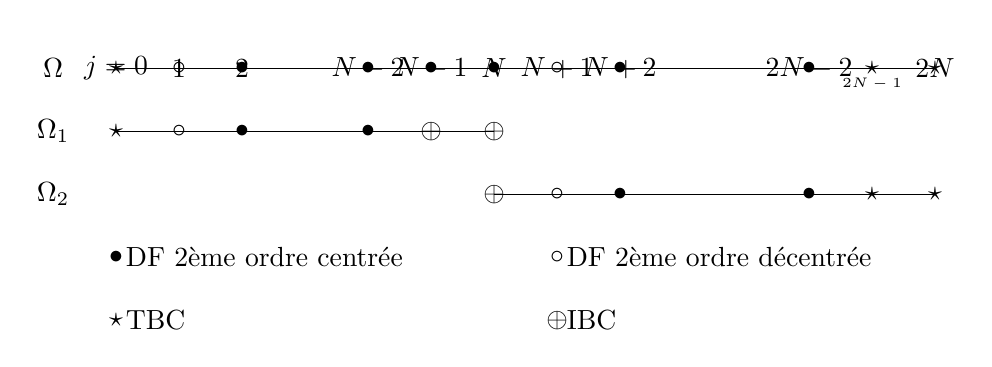
\begin{tikzpicture}[scale = .8]
	\coordinate (Alabel) at (-1,3);
	\coordinate (Aa) at (0,3);
	\coordinate (Ab) at (1,3);
	\coordinate (Ac) at (2,3);
	\coordinate (Ad) at (4,3);	
	\coordinate (Ae) at (5,3);	
	\coordinate (Af) at (6,3);	
	\coordinate (Ag) at (7,3);	
	\coordinate (Ah) at (8,3);	
	\coordinate (Ai) at (11,3);
	\coordinate (Aj) at (12,3);
	\coordinate (Ak) at (13,3);
	
	\draw (Aa) -- (Ak);
	\draw (Alabel) node {$\Omega$}; 
	\draw (Aa) node[label] {$j=0$};
	\draw (Ab) node[label] {$1$};
	\draw (Ac) node[label] {$2$};
	\draw (Ad) node[label] {$N-2$};
	\draw (Ae) node[label] {$N-1$};
	\draw (Af) node[label] {$N$};
	\draw (Ag) node[label] {$N+1$};
	\draw (Ah) node[label] {$N+2$};
	\draw (Ai) node[label] {$2N-2$};
	\draw (Aj) node[below,font=\tiny] {$2N-1$};
	\draw (Ak) node[label] {$2N$};
		
	\draw (Aa) node {$\star$};
	\draw (Ab) node {$\circ$};
	\draw (Aj) node {$\star$};
	\draw (Ak) node {$\star$};
	
	\draw (Ac) node{$\bullet$};
	\draw (Ad) node {$\bullet$};
	\draw (Ae) node {$\bullet$};
	\draw (Af) node{$\bullet$};	
	\draw (Ag) node{$\circ$};
	\draw (Ah) node {$\bullet$};
	\draw (Ai) node {$\bullet$};


	\coordinate (Blabel) at (-1,2);	
	\coordinate (Ba) at (0,2);
	\coordinate (Bb) at (1,2);
	\coordinate (Bc) at (2,2);
	\coordinate (Bd) at (4,2);	
	\coordinate (Be) at (5,2);	
	\coordinate (Bf) at (6,2);	

	\draw (Ba) -- (Bf); 
	
	\draw (Blabel) node {$\Omega_1$}; 
	\draw (Ba) node {$\star$};
	\draw (Bb) node {$\circ$};
	
	\draw (Bc) node {$\bullet$};
	\draw (Bd) node {$\bullet$};
	
	\draw (Be) node {$\oplus$};
	\draw (Bf) node {$\oplus$};	
	
	\coordinate (Clabel) at (-1,1);	
	\coordinate (Cf) at (6,1);	
	\coordinate (Cg) at (7,1);	
	\coordinate (Ch) at (8,1);	
	\coordinate (Ci) at (11,1);
	\coordinate (Cj) at (12,1);
	\coordinate (Ck) at (13,1);
		
	\draw (Cf) -- (Ck); 
	\draw (Clabel) node {$\Omega_2$}; 
	\draw (Cf) node{$\oplus$};
	\draw (Cg) node{$\circ$};
	\draw (Ch) node{$\bullet$};	
	\draw (Ci) node{$\bullet$};	
	\draw (Cj) node {$\star$};
	\draw (Ck) node{$\star$};
	
	%% Legend
	\draw (0,0) node {$\bullet$} node[right] {DF 2ème ordre centrée};
	\draw (7,0) node {$\circ$} node[right] {DF 2ème ordre décentrée};
	\draw (0,-1) node {$\star$} node[right] {TBC};
    \draw (7,-1) node {$\oplus$} node[right] {IBC};
	
\end{tikzpicture}
\captionof{figure}{Schéma indiquanla discrétisation spatiale imposée pour chaque point du monodomaine et des subdomaines de la DDM \label{fig:discretizations}}
\endgroup


\subsubsection{Numerical verification of the error}

\indent Le problème \eqref{eq:problemDDM1} - \eqref{eq:problemDDM2} a été résolu jusqu'à convergence avec cinq discrétisations spatiales uniformes différentes, au long d'un pas de temps (dans l'intervale $[0,\Delta t]$). Dans chaque cas, la solution de référence $u^{ref}$ était la solution du problème du monodomain \eqref{eq:problemMonodomain}, résolu avec la même taille de maille. Deux erreurs ont été calculées :

\begin{equation*}
	e^{N,*} = |u^{ref}_N - u^{*}_N|
\end{equation*}

\begin{equation}
	\label{eq:errorDDM}
	e^{\Omega,*} = ||u^{ref}_N - u^{*}_N||_2 = \sqrt{\Delta x \left[ \sum_{j=0}^N{(u^{ref}_j - u^{1,\infty}_j)^2 } + \sum_{j=N}^{2N}{(u^{ref}_j - u^{2,\infty}_j)^2 } \right] }
\end{equation}

\noindent correspondant respectivement à l'erreur sur l'interface et à l'erreur dans tout le domain.

\indent On s'intéresse au comportement de ces erreurs en fonction de la taille de maille. Comme montré la figure \ref{fig:orderVerification}, on vérifie que la DDM proposée par nous produit une erreur d'ordre $O(\Delta x)$  :

\begingroup
\begin{center}
	\includegraphics[scale=.5]{figures/convergenceVerificationCorrectN.png}
	\captionof{figure}{Vérification numérique de l'ordre de convergence de l'erreur due à la DDM \label{fig:orderVerification}}
\end{center}
\endgroup

\subsubsection{Corrections pour les TBCs approximées}

\indent On va formuler des modifications pour les TBCs utilisées dans l'ASM afin d'annuler ces erreurs :

\begin{equation*}
    \begin{gathered}
        \Theta_1^{c_L}(u_2^{n+1,k+1}) + \theta_1 = \Theta_1^{c_L}(u_1^{n,k}) + \theta_1' \\
        \Theta_2^{c_R}(u_1^{n+1,k+1}) + \theta_2 = \Theta_2^{c_R}(u_2^{n,k}) + \theta_2' \\
        \Theta_3^{c_R}(u_1^{n+1,k+1}) + \theta_3 = \Theta_3^{c_R}(u_2^{n,k}) + \theta_3'
    \end{gathered}
\end{equation*}

\noindent avec $\theta_i, \theta_i'$  donnés par 

\begin{gather*}
    \theta_1 = \Delta x c_L \frac{u_{N+1}^2 - 2u_{N}^2 + u_{N-1}^1}{\Delta x^2} + c_L^2\frac{\Delta x}{\Delta t} \left( u_{N}^2 - \alpha_{N}^2 \right)\\
    \theta_1' = - c_L^2\frac{\Delta x}{\Delta t} \left( u_{N}^1 - \alpha_{N}^1 \right)
\end{gather*}

\begin{equation*}
\begin{gathered}
    \theta_2 = \frac{\Delta x}{\Delta t} c_R^2 (u_N^1 - \alpha_N^1) \\
    \theta_2' = -\frac{\Delta x}{\Delta t} c_R^2 (u_N^2 - \alpha_N^2)
\end{gathered}
\end{equation*}

\begin{equation*}
\begin{gathered}
    \theta_3 = 2\frac{\Delta x}{\Delta t} \left[-\Delta x(u_{N-1}^1 - \alpha_{N-1}^1) - c_R (u_N^1 - \alpha_N^1) \right] + \Delta x \frac{u_{N-3}^1 - 2u_{N-2}^1 + u_{N-1}^1}{\Delta x^2} \\
    \theta_3' = 0
\end{gathered}
\end{equation*}

\indent En fait, on a, dans la convergence de la première condition à l'interface :

\begin{equation*}
\label{eq:modifiedTBC1}
\begin{aligned}
&& &    \Theta_1^{c_L}(u_N^*) + \theta_1 = \Theta_1^{c_L}(u_N^*) + \theta_1' \\
&& \implies &    u_N^* - c_L \frac{u_{N+1}^* - u_N^*}{\Delta x} + c_L^2\frac{u_N^* - 2u_{N+1}^* + u_{N+2}^*}{\Delta x^2} + \\ 
&& & \Delta x c_L \frac{u_{N+1}^* - 2u_{N}^* + u_{N-1}^*}{\Delta x^2} + c_L^2\frac{\Delta x}{\Delta t} \left( u_{N}^* - \alpha_{N}^* \right) = \\
&& & u_N^* - c_L \frac{u_{N}^* - u_{N-1}^*}{\Delta x} + c_L^2\frac{u_N^* - 2u_{N-1}^* + u_{N-2}^*}{\Delta x^2}  - c_L^2\frac{\Delta x}{\Delta t} \left( u_{N}^* - \alpha_{N}^* \right) \\
 && \implies &    2c_L^2 \frac{-\frac{1}{2}u_{N-2}^* + u_{N-1}^* - u_{N+1}^* + \frac{1}{2}u_{N+2}^* }{\Delta x ^2}  +             2c_L^2\frac{\Delta x}{\Delta t} \left( u_{N}^* - \alpha_{N}^* \right) = 0  \\
&& \implies &    \frac{u_{N}^* - \alpha_{N}^*}{\Delta t} + \frac{-\frac{1}{2}u_{N-2}^* + u_{N-1}^* - u_{N+1}^* + \frac{1}{2}u_{N+2}^* }{\Delta x ^3} = 0
\end{aligned}
\end{equation*}

\indent ce qui est identique à \eqref{eq:FDdiscretization} satisfaite dans $x_N$.

\indent Pour la deuxième IBC : 

\begin{equation}
\label{eq:modifiedTBC2}
\begin{aligned}
&& &\Theta_2^{c_R}(u_N^*) + \theta_2 = \Theta_2^{c_R}(u_N^*) + \theta_2'  \\
&& \implies & u_N^* - c_R^2 \frac{u_N^* - 2u_{N-1}^* + u_{N-2}^*}{\Delta x^2} + \frac{\Delta x}{\Delta t} c_R^2 (u_N^* - \alpha_N^*)  = \\ && & u_N^* - c_R^2 \frac{u_N^* - 2u_{N+1}^* + u_{N+2}^*}{\Delta x^2} -\frac{\Delta x}{\Delta t} c_R^2 (u_N^* - \alpha_N^*)  \\
&& \implies & 2\frac{\Delta x}{\Delta t} c_R^2 (u_N^* - \alpha_N^*) + 2c_R^2 \frac{-\frac{1}{2}u_{N-2}^* + u_{N-1}^* - u_{N+1}^* + \frac{1}{2}u_{N+2}^* }{\Delta x^2} = 0   \\
&& \implies &\frac{u_N^* - \alpha_N^*}{\Delta t} + \frac{-\frac{1}{2}u_{N-2}^* + u_{N-1}^* - u_{N+1}^* + \frac{1}{2}u_{N+2}^* }{\Delta x^3} = 0
\end{aligned}
\end{equation}

\noindent ce qui correspond également à \eqref{eq:FDdiscretization} satisfait dans $x_N$.

\indent Finalement, pour la troisième IBC, on utilise \eqref{eq:modifiedTBC2} dans \eqref{eq:TBCsIterOmega1B} pour obtenir

\begin{equation*}
-\frac{u_{N-1}^* - 2 u_{N}^* + u_{N+1}^*}{\Delta x} + 2c_R\Delta x\frac{u_N^* - \alpha_N^*}{\Delta t} = 0 
\end{equation*}

\indent Ainsi

\begingroup
\begin{align*}
\label{eq:modifiedTBC3}
&&  &\Theta_3^{c_R}(u_N^*) + \theta_3 = \Theta_3^{c_R}(u_N^*) + \theta_3'    \\
&& \implies & \frac{u_N^* - u_{N-1}^*}{\Delta x} + c_R \frac{u_N^* - 2u_{N-1}^* + u_{N-2}^*}{\Delta x^2} + 2\frac{\Delta x}{\Delta t}  \left[-\Delta x(u_{N-1}^* - \alpha_{N-1}^*) - c_R (u_N^* - \alpha_N^*) \right] + \\
&&   & 			\frac{u_{N-3}^* - 2u_{N-2}^* + u_{N-1}^*}{\Delta x}  =  \frac{u_{N+1}^* - u_{N}^*}{\Delta x} + c_R \frac{u_N^* - 2u_{N+1}^* + u_{N+2}^*}{\Delta x^2} \\
&&  \implies &  -\frac{u_{N-1}^* - 2 u_{N}^* + u_{N+1}^*}{\Delta x} + 2c_R\Delta_x\frac{u_N^* - \alpha_N^*}{\Delta t} + \\
&&   & 2\frac{\Delta x}{\Delta t} \left[-\Delta x(u_{N-1}^* - \alpha_{N-1}^*) - c_R(u_N^* - \alpha_N^*) \right] + \frac{u_{N-3}^* - 2u_{N-2}^* + u_{N-1}^*}{\Delta x} = 0 \\
&& \implies  & -2\frac{-\frac{1}{2}u_{N-3}^* + u_{N-2}^* - u_{N}^* + \frac{1}{2}u_{N+1}^* }{\Delta x} - 2\frac{\Delta x^2}{\Delta t}(u_{N-1}^* - 					\alpha_{N-1}^*) = 0 \\
&& \implies &  \frac{u_{N-1}^* - \alpha_{N-1}^*}{\Delta t} + \frac{-\frac{1}{2}u_{N-3}^* + u_{N-2}^* - u_{N}^* + \frac{1}{2}u_{N+1}^* }{\Delta x ^3} = 0
\end{align*}
\endgroup

\noindent ce qui est la discrétisation \eqref{eq:FDdiscretization} écrite pour le point $x_{N-1}$.

\subsection{Optimisation des IBCs (vitesse de convergence)}

\indent Notre objectif maintenant est d'optimiser les IBCs, dans le sens de minimiser le nombre de itérations de l'ASM pour arriver à la convergence.   Ainsi, de façon similaire à l'optimisation des TBCs faite dans la section \ref{sec:approxTBC}, on va faire un très large ensemble de tests, afin de trouver les coefficients $c_L$ et $c_R$ qui fournissent la convergence la plus rapide. Dans un permier moment, on fera cet étude avec un pas de temps et un pas de espace fixés, afin d'analyser exclusivement l'influence du coefficient; en suite, on va introduire ces deux paramètres dans l'étude.

\indent Comme on connait une solution de référence, le critère de convergence utilisé est

\begin{equation*}
\label{eq:criteriaConvergence}
	e^{\Omega,k} \leq \epsilon
\end{equation*}

\noindent avec $\epsilon = 10^{-9}$ et  l'erreur $e^{\Omega,k}$, pour chaque itération $k$, définie comme dans \eqref{eq:errorDDM}.

\indent Afin de simplifier les tests et d'éviter des coûts de calcul trop élevés,  on va considérer toujours $c_L = c_R = c$  dans le procès d'optimisation. Le range des coefficients testés est $[-10.0, 20.0]$ (choisi après des tests initiaux pour identifier un intervalle approprié), avec un pas égal à  $0.1$ entre eux (ou encore plus petit, jusqu'à $0.005$, dans les régions proches des coefficients optimaux). Le nombre maximal d'itérations est 100.

\indent Comme une dernière remarque, on rappelle que tous les tests seront réalisées au long d'un seul pas de temps.

\subsubsection{Tests variant l'instant initial et la position de l'interface}

\indent On va utiliser un pas de temps $\Delta t = 20/2560 = 0.0078125$ et une taille de maille $\Delta x = 12/500 = 0.024$ fixés. Par ailleurs, on va mettre en place deux ensembles de tests, qui nous permettront d'étudier la vitesse de convergence avec des différentes conditions initiales et différents tailles des subdomaines :

\begin{enumerate}
	\item Tests variant l'instant initial $t_0$, avec l'interface fixée sur le centre du monodomaine $\Omega = [-6,6]$;
	\item Tests variant la position de l'interface ($x_{interface} = -L + \alpha 2L$, où  $L = 6$ et $0 < \alpha < 1$), pour un instant initial $t_0 = 0.78125$. fixé.
\end{enumerate}

\indent Dans tous les cas, la solution de référence $u^{ref}$ sera la solution du problème dans le monodomaine \eqref{eq:problemMonodomain}, calculée dans $[t_0,t_0 + \Delta t]$.

\indent Les résultats obtenus sont résumés dans les figures \ref{fig:optimVarT0} and \ref{fig:optimVarInterface}, avec le nombre d'itérations en fonction du coefficient $c$. Par souci de clarité, les résultats pour les coefficients négatifs et positifs sont présentés dans des graphes séparés. Ils montrent des comportements très similaires pour toutes les courbes, avec deux minima for $c < 0$ et deux autres for $c > 0$, avec approximativement la même valeur dans tous les cas (environ -1.35, -0.10, 0.20 and 4.50). Les minima les plus proches de zéro sont associés à des courbes très discontinues, tandis que les autres deux minima sont associés à des courbes plus lisses (voir les détails dans les figures \ref{fig:optimVarT0NDetail}-\ref{fig:optimVarT0PDetail2} et \ref{fig:optimVarInterfaceNDetail}-\ref{fig:optimVarInterfacePDetail2}). Finalement, on remarque que, pour quelques courbes, le minimum est associée aux coefficients les plus proches de zéro, et pour les autres courbes, il est associée aux autres coefficients. Néanmoins, dans tous ces cas, les nombres optimales d'itérations sont similaires (entre cinq et sept).

\begingroup
\noindent
\begin{minipage}[t]{.45\linewidth}
	\includegraphics[scale=.4]{figures/FinalFigures/NiterxCoefVarT0FinalVersionN.png}
	\captionof{subfigure}{Vue générale des coefficients négatifs}
\end{minipage}
\hfill
\begin{minipage}[t]{.45\linewidth}
	\includegraphics[scale=.4]{figures/FinalFigures/NiterxCoefVarT0FinalVersionP.png}
	\captionof{subfigure}{Vue générale des coefficients positifs}
\end{minipage}
\begin{minipage}[t]{.45\linewidth}
	\includegraphics[scale=.4]{figures/FinalFigures/NiterxCoefVarT0FinalVersionNDetail.png}
	\captionof{subfigure}{Détail autour d'un des coefficients optimaux négatifs  \label{fig:optimVarT0NDetail}}
\end{minipage}
\hfill
\begin{minipage}[t]{.45\linewidth}
	\includegraphics[scale=.4]{figures/FinalFigures/NiterxCoefVarT0FinalVersionNDetail2.png}
	\captionof{subfigure}{Détail autour de l'autre coefficient optimal négatif  \label{fig:optimVarT0NDetail2}}
\end{minipage}
\begin{minipage}[t]{.45\linewidth}
	\includegraphics[scale=.4]{figures/FinalFigures/NiterxCoefVarT0FinalVersionPDetail.png}
	\captionof{subfigure}{Détail autour d'un des coefficients optimaux positifs \label{fig:optimVarT0PDetail} }
\end{minipage}
\hfill
\begin{minipage}[t]{.45\linewidth}
	\includegraphics[scale=.4]{figures/FinalFigures/NiterxCoefVarT0FinalVersionPDetail2.png}
	\captionof{subfigure}{Détail autour de l'autre coefficient optimal positif   \label{fig:optimVarT0PDetail2}}
\end{minipage}
	\captionof{figure}{Nombre d'itérations jusqu'à convergence en fonction du coefficient des TBCs, pour une interface fixée et des différentes valeurs de $t_0$  \label{fig:optimVarT0}}
\endgroup

\begingroup
\noindent
\begin{minipage}{.45\linewidth}
	\includegraphics[scale=.4]{figures/FinalFigures/NiterxCoefVarInterfaceFinalVersionN.png}
	\captionof{subfigure}{Vue générale des coefficients négatifs}
\end{minipage}
\hfill
\begin{minipage}{.45\linewidth}
	\includegraphics[scale=.4]{figures/FinalFigures/NiterxCoefVarinterfaceFinalVersionP.png}
	\captionof{subfigure}{Vue générale des coefficients positifs}
\end{minipage}
\begin{minipage}{.45\linewidth}
	\includegraphics[scale=.4]{figures/FinalFigures/NiterxCoefVarInterfaceFinalVersionNDetail.png}
	\captionof{subfigure}{Détail autour d'un des coefficients optimaux négatifs  \label{fig:optimVarInterfaceNDetail}}
\end{minipage}
\hfill
\begin{minipage}{.45\linewidth}
	\includegraphics[scale=.4]{figures/FinalFigures/NiterxCoefVarInterfaceFinalVersionNDetail2.png}
	\captionof{subfigure}{Détail autour de l'autre coefficient optimal négatif  \label{fig:optimVarInterfaceNDetail2}}
\end{minipage}
\begin{minipage}{.45\linewidth}
	\includegraphics[scale=.4]{figures/FinalFigures/NiterxCoefVarInterfaceFinalVersionPDetail.png}
	\captionof{subfigure}{Détail autour d'un des coefficients optimaux positifs \label{fig:optimVarInterfacePDetail}  }
\end{minipage}
\hfill
\begin{minipage}{.45\linewidth}
	\includegraphics[scale=.4]{figures/FinalFigures/NiterxCoefVarInterfaceFinalVersionPDetail2.png}
	\captionof{subfigure}{Détail autour de l'autre coefficient optimal positif  \label{fig:optimVarInterfacePDetail2}}
\end{minipage}
	\captionof{figure}{Nombre d'itérations jusqu'à convergence en fonction du coefficient des TBCs, pour $t_0$ fixé et des différentes positions de l'interface \label{fig:optimVarInterface}}
\endgroup

\indent La figure \ref{fig:errorEvolution} montre l'évolution de l'erreur, en fonction des itérations, pour cinq coefficients $c$ qui ont fournit les convergences les plus rapides, pour un temps initial et une position de l'interface fixés. Pour des autres valeurs de $t_0$ et $\alpha$, le graph est similaire, en ce qui concerne le nombre d'itérations et le fait que la convergence est plus régulière pour les coefficients les plus proches de zéro, en comparaison aux autres coefficients optimaux.

\begingroup
\begin{center}
\includegraphics[scale=.5]{figures/FinalFigures/errorEvolutionFixedT0BFinalVersion.png}
\captionof{figure}{Évolution de l'erreur, en fonction des itérations, pour les tests les plus rapides \label{fig:errorEvolution}}
\end{center}
\endgroup

\subsubsection{Tests variant $\Delta t$ and $\Delta x$}

\indent Après vérifier que la méthode se comporte de façon similaire pour toute condition initiale (i.e., pour tout $t_0$) et toute position de l'interface, on a fixé ces paramètres ($t_0 = 0$ and $\alpha = 0.5$) et on a fait des nouveaux tests avec des différentes valeurs de $\Delta t$ (avec $\Delta x = 12/250$ fixé) et des différentes valeurs de $\Delta x$ (avec $\Delta t = 0.02$ fixé).

\indent Le nombre d'itérations en fonctions des coefficients, pour quelques tests, est montré dans les figures \ref{fig:niterxCoefVarDt} et \ref{fig:niterxCoefVarDx}. La figure \ref{fig:optimalCoefVarDxDtCorrectN} présente le coefficient optimal pour chaque $\Delta t$ ou $\Delta x$. En considérant la remarque qu'on a fait concernant les résultats similaires (i.e., le nombre d'itérations jusqu'à convergence) pour les quatre coefficients optimaux, on a tenu en compte, pour la construction des courbes de la figure \ref{fig:optimalCoefVarDxDtCorrectN}, seulement les minima les plus lointains de zéro: ceci a été fait parce que, comme montre les figures \ref{fig:niterxCoefVarDt} et \ref{fig:niterxCoefVarDx}, ces minima ont une forte dépendance de $\Delta t$ et $\Delta x$, et on va chercher à étudier cette relation.

\begingroup
\noindent
\begin{minipage}{.45\linewidth}
	\includegraphics[scale=.45]{figures/FinalFigures/NiterxCoefVarDtdx250FinalVersionNMarshal.png}
\captionof{subfigure}{Coefficients négatifs}
\end{minipage}
\hfill
\begin{minipage}{.45\linewidth}
	\includegraphics[scale=.45]{figures/FinalFigures/NiterxCoefVarDtdx250FinalVersionPMarshal.png}
\captionof{subfigure}{Coefficients positifs}
\end{minipage}
\captionof{figure}{Nombre d'itérations jusqu'à convergence en fonction du coefficient pour $2N = 250$ fixé et des différentes valeurs de $\Delta t$  \label{fig:niterxCoefVarDt}}
\endgroup

\begingroup
\noindent \begin{minipage}{.45\linewidth}
	\includegraphics[scale=.45]{figures/FinalFigures/NiterxCoefVarDxdt2em2FinalVersionN.png}
\captionof{subfigure}{Negative coefficients}
\end{minipage}
\hfill
\begin{minipage}{.45\linewidth}
	\includegraphics[scale=.45]{figures/FinalFigures/NiterxCoefVarDxdt2em2FinalVersionP.png}
\captionof{subfigure}{Positive coefficients}
\end{minipage}
\captionof{figure}{Nombre d'itérations jusqu'à convergence en fonction du coefficient des TBCspour $\Delta t = 0.02$ et des différentes valeurs de $\Delta x$  \label{fig:niterxCoefVarDx}}
\endgroup


\begin{center}
	\includegraphics[scale=.5]{{figures/FinalFigures/OptimalCoefVarDxDtFinalVersionMarshal.png}}
	\captionof{figure}{Coefficients optimaux en fonction du pas de temps et de la taille de maille\label{fig:optimalCoefVarDxDtCorrectN}}
\end{center}

\indent La figure \ref{fig:optimalCoefVarDxDtCorrectN} suggère que le coefficient optimal dépende de $(\Delta t)^\nu$ et $(\Delta x)^\eta$, avec $0 \leq \nu \leq 1$ et $\eta < 0$. En fait, en faisant quelques régressions avec $\Delta t $ ou $\Delta x$ fixé, on peut conclure que $\nu = \frac{2}{3}$ et $\eta = -1$ fournissent des courbes de régression très bien adaptées (avec des coefficients de détermination $R^2$ plus grandes que 0.99), pour les cas des coefficients positifs et négatifs (même que chacun de ces cas corresponde à des courbes différents). Ainsi, on va chercher à modéliser une fonction

\begin{equation}
	\label{eq:regression2D}
	c_{opt}(\Delta t, \Delta x) = \kappa + \alpha (\Delta t)^{\frac{2}{3}} + \beta \frac{1}{\Delta x} + \gamma   \frac{(\Delta t)^{\frac{2}{3}}}{\Delta x}
\end{equation}

\indent Une régression utilisant les coins du rectangle $[0.001,0.1]\times[\frac{12}{100},\frac{12}{1000}]$ et quinze points à l'intérieur fournit les surfaces 

\begin{gather}
	c_{opt}^+(\Delta t, \Delta x) = 0.0775 -0.3353 (\Delta t)^{\frac{2}{3}} - 0.0012 \frac{1}{\Delta x} + 2.7407   \frac{(\Delta t)^{\frac{2}{3}}}{\Delta x} 	\label{eq:regression2DPos} \\
	c_{opt}^-(\Delta t, \Delta x) = -0.0583 -1.5024 (\Delta t)^{\frac{2}{3}} - 0.0006 \frac{1}{\Delta x} -0.7287  \frac{(\Delta t)^{\frac{2}{3}}}{\Delta x} 	\label{eq:regression2DNeg}
\end{gather}

\noindent respectivement pour les coefficients optimaux positifs et négatifs. Les coefficients de détermination de chaque régression son $R^{2,+} = 0.9999894$ et $R^{2,-} = 0.9998993$, ce qui indique une bonne représentation.

\indent Afin de valider les expressions \eqref{eq:regression2DPos} and \eqref{eq:regression2DNeg}, elles ont été utilisées pour calculer le coefficient optimaux pour des plusieurs points $(\Delta t, \Delta x)$, avec $\Delta t \in [0.0005,0.3]$ et $\Delta x \in \left[ \frac{12}{5000},\frac{12}{50} \right]$. Comme montre la figure \ref{fig:regressionValidation}, pour la plupart des points dans le domaine considéré, le coefficient optimal calculé fournit une convergence rapide vers la solution du monodomaine, avec moins de 20 itérations (ou encore moins que 12 itérations), sur une grand région du domaine).

\begingroup
\noindent
\begin{minipage}[t]{.45\linewidth}
	\includegraphics[scale=.45]{figures/FinalFigures/contourValidationN.png}
	\captionof{subfigure}{Coefficients négatifs}
\end{minipage}
\hfill
\begin{minipage}[t]{.45\linewidth}
	\includegraphics[scale=.45]{figures/FinalFigures/contourValidationP.png}
	\captionof{subfigure}{Coefficients positifs}
\end{minipage}
\captionof{figure}{Lignes de contour du nombre d'itérations jusqu'à convergence, en utilisant les coefficients optimaux $c_{opt}^+(\Delta t, \Delta x)$ obtenus à partir des régressions. \label{fig:regressionValidation}}.
\endgroup

\indent Les nombres d'itérations montrées dans la figure \ref{fig:regressionValidation} ne sont pas les plus petites qu'on est capable de trouver (cf. les figures \ref{fig:optimVarT0Interface} jusqu'à \ref{fig:niterxCoefVarDtDx}), parce que les expressions \eqref{eq:regression2DPos} et \eqref{eq:regression2DNeg} sont des régressions construites à partir de coefficients optimaux obtenus parmi un ensemble discret de valeurs possibles. Néanmoins, elles donnent des très bonnes approximations pour le $c$ optimal pour chaque $(\Delta t, \Delta x)$, et ainsi on peut chercher dans une petite région autour du $c_{opt}$ calculé pour obtenir une convergence encore plus rapide.

\subsection{Partial conclusion}
 
\indent The results presented in this section show that the Domain Decomposition Method proposed here, consisting in the Additive Schwarz Method with our approximate TBCs, is able to provide a fast convergence toward the solution of the monodomain problem. Therefore, we reached our goals of solving the dispersion equation in a finite domain divided in two subdomains.

\indent Moreover, the results of the optimization tests are very satisfying regarding a more general application of our method. Firstly, for fixed spatial and temporal discretizations, we obtained optimal coefficients for the method independently of the initial solution and the size of the subdomains (i.e., independently of the initial instant and the position of the interface). Secondly, we obtained good regression curves for the optimal coefficient as function of $\Delta t$ or $\Delta x$, which could allow the application of the model, with fast convergence, for tests different for the ones made in this study.

\section{Conclusion}


\indent We presented and implemented in this paper a domain decomposition method, using approximate transparent boundary conditions as interface  conditions between the subdomains, for the resolution of a one dimensional dispersive evolution equation. Although not as accurate (in the role of TBCs) as the ones proposed in the works we are based on (providing better TBCs was not our objective here), these approximate conditions stand out for its simple form and implementation and the fast convergence that they provide for the Schwarz method. Moreover, we also proposed small corrections to them, which insure that the solution of the DDM problem converges exactly to the solution of the monodomain problem. Finally, we verified that the speed of convergence depends on the time step, the mesh size and the (only) coefficient for constructing the approximate interface conditions; thus, via an optimization process, we obtained and validated regression expressions that provide the optimal coefficient (\emph{i.e.}, the one that provides the fastest convergence) in function of $\Delta t $ and $\Delta x$.

\indent Natural continuations of the work presented here would be its extension to other problems, for example the linearized KdV equation, which adds an advective term on the equation solved here, as well as other models of wave propagation.

\newpage
\part*{Bilan personnel}
\addcontentsline{toc}{part}{Bilan personnel}

\indent J'avais choisi ces deux stages en espérant avoir des missions et expériences correspondantes à mes perspectives professionnelles : j'envisage une carrière dans la recherche en mathématiques appliquées, plus spécifiquement sur des méthodes numériques pour des équations différentielles, avec des applications à des problèmes de la mécanique des fluides (des thématiques que m'intéressent beaucoup et avec lesquelles j'avais déjà une expérience précédente). Maintenant, après la conclusion de l'année de césure, je peux affirmer que ces deux stages ont confirmé et renforcé ces perspectives et ma passion pour la recherche scientifique, en me donnant encore plus envie de poursuivre cette carrière.

\indent J'ai eu l'occasion de connaître plus profondément les plus variés aspects du monde de la recherche. D'abord, le fait de qu'il y a toujours quelque chose de nouveau à faire, à corriger ou à découvrir. Quand on se pose un objectif, pour y arriver il faut beaucoup étudier, écrire, programmer, tester et déboguer. Et quand on y arrive, on s'aperçoit qu'on peut toujours passer à des nouveaux cas, à des modèles plus complexes et comparer avec ce qui a été déjà fait par des autres scientifiques. Par ces mêmes raisons, j'ai pu vérifier que le travail dans la recherche se caractérise pour avoir, en citant Antoine Rousseau, un rythme de production complètement inconstant : parfois j'ai avancé très rapidement, mais j'ai aussi passé des semaines pour résoudre des petits problèmes. Dans tous les cas, c'était toujours des motivations pour poursuivre le travail.

\indent Un autre très important aspect que j'ai connu dans les deux stages est la multidisciplinarité qui peut se développer dans la recherche scientifique. À Bordeaux, des chercheurs et des étudiants de plusieurs domaines composaient l'équipe CARDAMOM, et, à Santiago, j'étais fortement impressionné quand j'ai connu toutes les lignes de recherche dans MERIC pour l'étude de la production d'énergie marine, dont la plupart je ne connaissais pas auparavant. Ainsi, je me suis rendu compte que mon travail, dans les deux stages et aussi dans le futur, n'est qu'une petite partie de ce qui peut être étudié dans la recherche.

\indent Un dernier point à remarquer sur ce contact avec la recherche scientifique, et qui constitue une des principales raisons qui ont confirmé mon intéresse dans ce domaine, est la très bonne ambiance de travail. Mes orientateurs et mes collègues d'équipe étaient toujours prêts à m'écouter et à m'aider et enseigner quand j'avais besoins. J'ai eu toujours l'occasion de proposer mes idées et de guider mon travail selon mes préférences.

\indent Dans ce qui concerne les expériences et connaissances techniques acquises dans les stages, j'ai beaucoup appris et j'ai renforcé des compétences et connaissances sur des aspects mathématiques et numériques, en complémentant ce que j'avais appris à l'École des Ponts.

\indent À Bordeaux, j'ai travaillé à fond avec des modèles d'adaptation de maillage, qui étaient complètement nouveaux pour moi. En implémentant ces modèles avec des méthodes d'éléments finis, j'ai pu me familiariser à ce type de méthode, y compris ses aspects théoriques (la dérivation de la méthode à partir de la formulation variationnelle du problème) et pratiques (comme le calcul des éléments de la matrice du système linéaire, le stockage de la matrice creuse, le traitement des entités géométriques en deux et trois dimensions, etc.). Finalement, la création d'une bibliothèque m'a donné une forte expérience concernant le développement logiciel, la structure et spécificités de la langage C, les aspects liés à la compilation des programmes et le travail en utilisant Git pour gérer les versions et travailler en équipe.

\indent À Santiago, même en travaillant avec des sujets avec lesquels j'étais déjà plus familiarisé, j'ai eu aussi un premier contact avec des nouveaux concepts, comme les modèles de propagation des ondes qu'on a considéré, les conditions aux bords transparentes et les méthodes de décomposition de domaine. Par rapport au stage à Bordeaux, où mes tâches étaient plutôt numériques, je considère qu'à Santiago j'ai travaillé de façon plus équilibrée entre les côtés mathématique et numérique, ce qui aura certainement une grande importance dans la suite de ma formation académique.

\indent Dans tous les cas, le contact et les discussions avec les orientateurs, les étudiants qui intégraient mes équipes de travail et d'autres chercheurs ont été essentielles pour consolider les connaissances acquises dans les stages.

\indent Toujours concernant les compétences acquises, je fais une remarque spéciale sur la production de textes scientifiques. Au long des deux stages, j'ai constamment rédigé des rapports pour enregistrer et organiser les achèvements, tests et conclusions réalisés. Notamment, dans le deuxième stage j'ai écrit mon premier papier scientifique, qu'on a envoyé pour sa publication, et j'ai connu les plusieurs difficultés impliquées dans cette tâche : l'organisation, sélection et présentation de l'information, en pensant que texte sera lu par d'autres personnes, possiblement pas familiarisés avec le sujet; les constantes révisions; et le propre fait, aussi en citant Antoine Rousseau, ``qu'un papier n'est jamais fini".

\indent D'un point de vue moins technique, mais également important, le déroulement des stages en différentes villes et pays a complété l'expérience de l'année de césure. Je remarque notamment l'exercice au niveau linguistique : dans les deux stages, j'ai eu l'occasion de développer mon français et mon anglais, et aussi l'espagnol au Chili. Par ailleurs, dans le deuxième stage, j'ai pu aussi connaître un autre mode de vie et une autre culture.

\indent Finalement, en tenant compte des discussions et des \emph{feedbacks} faits au long et à la fin des stages par mes orientateurs et les autres membres des équipes, je crois que j'ai apporté des importantes contributions à ses activités de recherche, ce qui est très motivateur et certainement me stimulera à continuer à travailler dans ce domaine. À Bordeaux, on a beaucoup avancé sur la bibliothèque d'adaptation de maillage, qui peut être déjà utilisée dans des codes de mécaniques de fluides, étant ainsi utiles aux chercheurs et thésards de l'équipe; et au Chili, on est arrivé à des très bons résultats pour la décomposition de domaine appliquée à un des modèles de propagation  d'onde, ce qui peut guider les prochaines pas de MERIC dans la ligne de la modélisation mathématique pour l'énergie marine.
\bibliography{../may/biblio}
\end{document}
